% arara: xelatex: { synctex: true, shell: true }
% arara: bibtex
% arara: xelatex: { synctex: true, shell: true }
% arara: xelatex: { synctex: true, shell: true }
\documentclass[thesis=M,slovak]{FITthesis}[2019/03/21]
\OnehalfSpacing
\raggedbottom % no huge vertical whitespace between elements on short pages

\usepackage{dirtree}
\usepackage{lipsum,tikz}
\usepackage[utf8]{inputenc} 
\usepackage{dirtree}
\usepackage{amsmath}
\usepackage{xevlna}
\usepackage{luavlna}
\usepackage{float}
\usepackage{todonotes}
\usepackage{array}
\usepackage{fnpct}
\usepackage{float}
\usepackage{listings} % typesetting of sources
\usepackage{csquotes}
\usepackage{bookmark}

\usepackage[style=iso-numeric]{biblatex}
\addbibresource{bib-database.bib}

\RequirePackage[labelsep=space,singlelinecheck=false,font={up,small},labelfont={sf,bf}]{caption}[2020/05/30]

\usepackage[hypcap=true]{caption} % fix for figure and table label positioning in PDF
\BeforeBeginEnvironment{figure}{\vskip\baselineskip}
\BeforeBeginEnvironment{listing}{\vskip\baselineskip}
\BeforeBeginEnvironment{table}{\vskip\baselineskip}
\setlength{\intextsep}{6pt}

\usepackage[chapter]{minted}
\setminted{autogobble=true,fontsize=\footnotesize,tabsize=4}
\usemintedstyle{xcode}
\newmintinline[code]{text}{}

\setlength{\parindent}{0pt}
\abnormalparskip{\baselineskip}

\usepackage{enumitem}

\setlist[1]{before={\parskip=0pt}}

% custom hyphenation
\hyphenation{rádio-frekvenčné}
\hyphenation{n-dimen-zio-nál-nych}
\hyphenation{ces-ty}

\department{Katedra softwarového inženýrství}
\title{Webové rozhranie pre spracovanie SPAMM tagovaných dát z magnetickej rezonancie}
\authorGN{Tomáš} 
\authorFN{Taro}
\authorWithDegrees{Bc. Tomáš Taro} 
\author{Tomáš Taro}
\supervisor{Ing. Petr Pauš, Ph.D.}
\acknowledgements{}
\abstractCS{}
\abstractEN{}
\placeForDeclarationOfAuthenticity{V~Prahe}
\declarationOfAuthenticityOption{1} 
\keywordsCS{}
\keywordsEN{}

\begin{document}	
        \begin{introduction}
TODO
\end{introduction}

        \chapter {Magnetická rezonancia}
Magnetická rezonancia (MR) je jedna zo zobrazovacích techník, ktorá je používaná k zobrazeniu vnútorných orgánov tela.
Narozdiel od röntgenového žiarenia a počítačovej tomografie (CT), magnetická rezonancia nepoužíva ionizujúce žiarenie. Avšak medzi spoločné znaky týchto troch zobrazovacích techník patrí ich neinvazívnosť a bezbolestné vyšetrenie \cite{basic_principles_of_mri} (vlastný preklad).

Magnetická rezonancia sa používa najmä pri:
\begin {itemize}
\item {podozrení na anomálie mozgu a miechy, nádory a cysty,}
\item {poranení kĺbov a mäkkých tkanív,}
\item {podozrení na srdcové problémy a}
\item {pri rozličných ochoreniach pečene a iných brušných orgánov \cite{mr_usage} (vlastný preklad).}
\end {itemize}

Pred niektorými MR procedúrami sa pacientovi môže intravenózne podať kontrastná látka, ktorá zlepší kontrast a vzájomnú odlíšiteľnosť orgánov \newline a mäkkých tkanív \cite{contrast_agents}.

Bohužiaľ, existujú aj určité kontraindikácie, pri ktorých použitie MR nie je pre človeka vhodné.
Jedným z kontraindikácií je implantovaný kardiostimulátor, v prípade že nie je kompatibilný s MR prístrojom.
\clearpage

Všeobecne sa za kontraindikáciu považuje použitie akéhokoľvek magnetického materiálu v tele. Taktiež je MR vyšetrenie kontraindikované ženám v prvom trimestri tehotenstva \cite{mr_contraindications}.

\section {Princíp magnetickej rezonancie}
Princípom magnetickej rezonancie je smerové magnetické pole (moment - $\mathcal{B}_{0}$) spojené s pohybom voľných jadier vodíku v tele pacienta. Tieto jadrá majú charakteristický pohyb (spin) vytvárajúci malý magnetický moment s určitým náhodným smerom a veľkosťou  \cite{basic_principles_of_mri} (vlastný preklad).

Keď je pacient umiestnený vo veľkom magnetickom poli (v tubuse MR prístroja), voľné vodíkové jadrá sa zarovnajú v smere $\mathcal{B}_{0}$ (smer $y$) a vytvoria magnetický moment $\mathcal{M}$ paralelne k $\mathcal{B}_{0}$. Vodíkové jadrá začnú náhle prechádzať okolo smeru magnetického pola ako gyroskopy. Toto správanie sa nazýva Larmorova precesia \cite{basic_principles_of_mri} (vlastný preklad).

\begin {figure}[H]
        \centering
        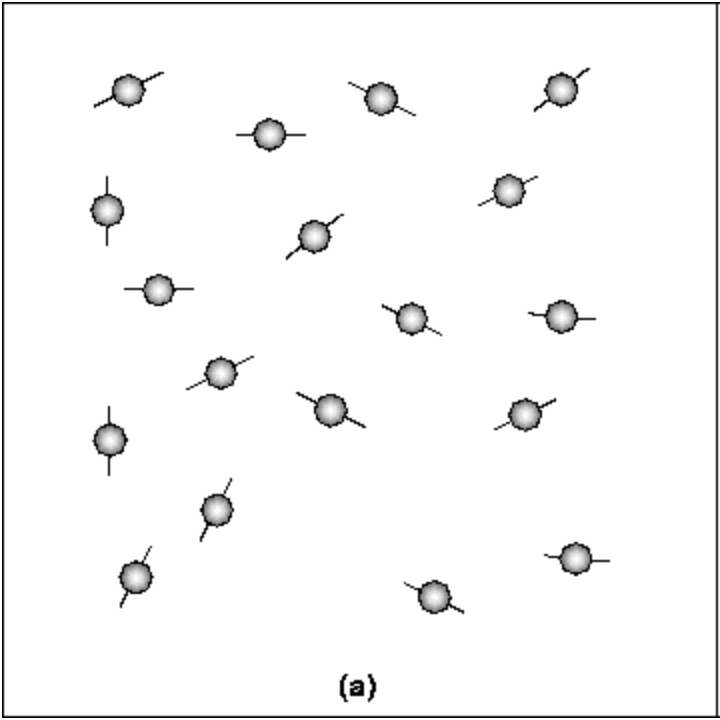
\includegraphics[height=6cm]{media/hydrogen/hydrogen_moving_freely.png}
        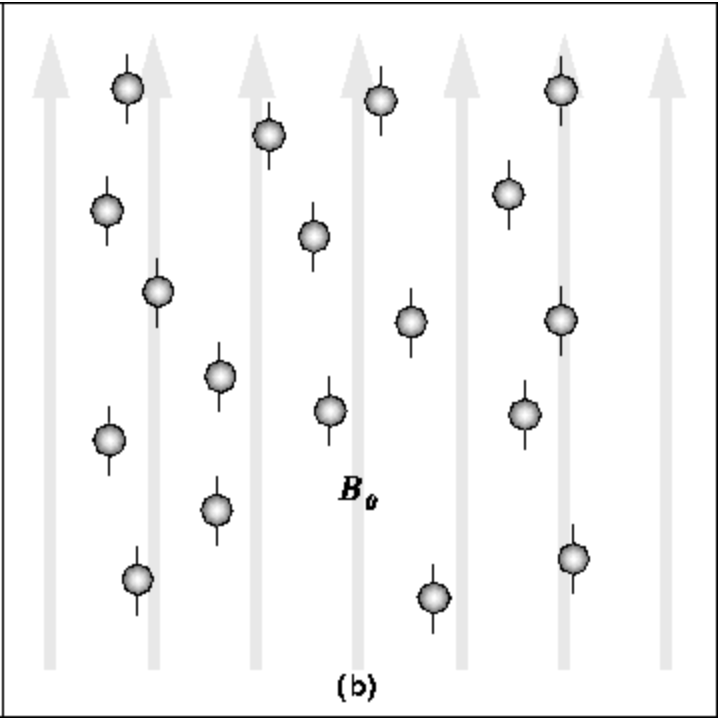
\includegraphics[height=6cm]{media/hydrogen/hydrogen_oscilating.png}
        \captionsetup{justification=centering}
        \captionof{figure}[Voľný pohyb vodíkových jadier a ich zarovnanie v smere $\mathcal{B}_{0}$]{Na ľavom obrázku je možné vidieť voľný pohyb vodíkových jadier,\newline na pravom obrázku ich zarovnanie v smere $\mathcal{B}_{0}$ \cite{basic_principles_of_mri}.}
\end {figure}

Následne sa aplikuje rádiofrekvenčný impulz $\mathcal{B}_{rf}$ kolmo na $\mathcal{B}_{0}$. \newline
Tento impulz rovnajúci sa frekvencii Larmorovej precesie spôsobí posun \newline $\mathcal{M}$ od $\mathcal{B}_{0}$ \cite{basic_principles_of_mri} (vlastný preklad).

\clearpage

Frekvencia Larmorovej precesie, tzv. Larmorova frekvencia, je definovaná ako:
\begin {center}
$\omega_{0}$ = $-\gamma * \mathcal{B}_{0}$,
\end {center}

kde $\gamma$ predstavuje gyromagnetický pomer a $\mathcal{B}_{0}$ intenzitu magnetického pola.
Gyromagnetický pomer je konštanta závislá na jadre danej častice. \newline Pre vodík sa táto konštanta rovná 42.6 MHz/Tesla \cite{basic_principles_of_mri} (vlastný preklad).

\begin {figure}[H]
        \centering
        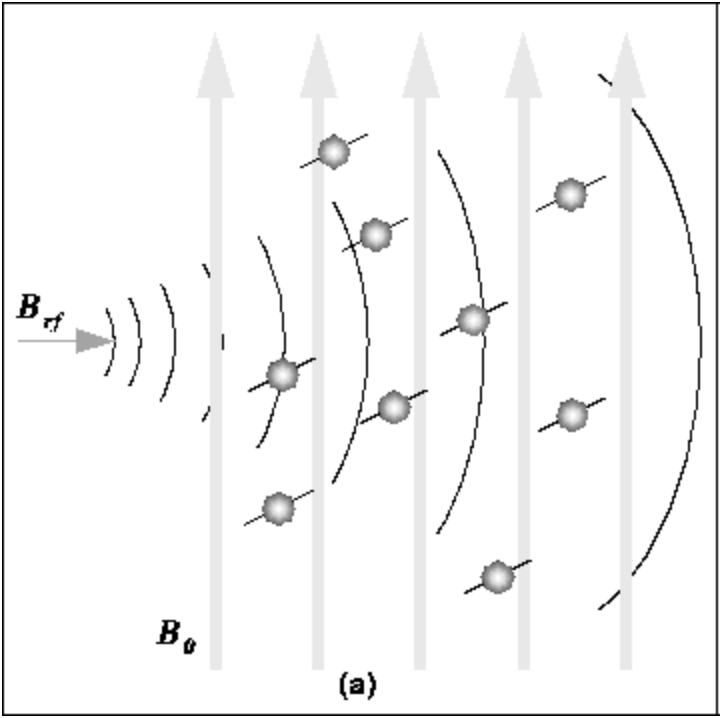
\includegraphics[height=6cm]{media/hydrogen/hydrogen_reacting_to_rf.png}
        \captionsetup{justification=centering}
        \captionof{figure}[Kolmá aplikácia RF impulzu $\mathcal{B}_{rf}$ na vodíkové jadrá]{Kolmá aplikácia RF impulzu $\mathcal{B}_{rf}$ na vodíkové jadrá \cite{basic_principles_of_mri}.}
\end {figure}

Akonáhle prestane pôsobiť rádiofrekvenčný impulz $\mathcal{B}_{rf}$, vodíkové jadrá sa presunú naspäť tak, že ich $\mathcal{M}$ je znovu paralelný s $\mathcal{B}_{0}$. Tento návrat vodíkových jadier sa nazýva relaxácia. Počas nej jadrá strácajú energiu vysielaním ich vlastného rádiofrekvenčného signálu  \cite{basic_principles_of_mri} (vlastný preklad).

Tento signál sa nazýva \uv{voľný indukčný rozpad} -- z anglického Free Induction Decay (FID). Ten sa zmeria vodivým poľom MR prístroja za účelom vyhotovenia 3D MR snímky v odtieňoch šedej \cite{basic_principles_of_mri} (vlastný preklad).

\begin {figure}[H]
        \centering
        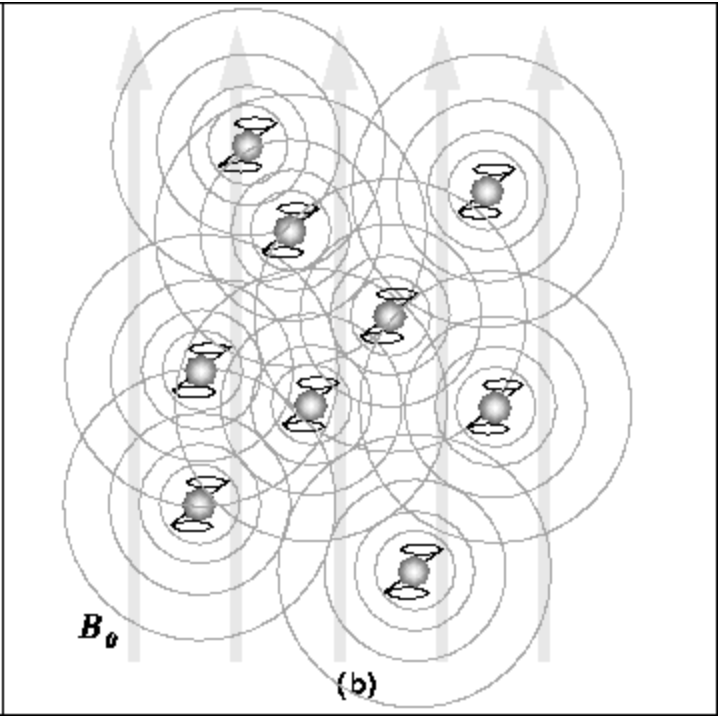
\includegraphics[height=6cm]{media/hydrogen/hydrogen_emitting_rf.png}
        \captionsetup{justification=centering}
        \captionof{figure}[Emitovanie FID signálu vodíkovými jadrami]{Emitovanie FID signálu vodíkovými jadrami \cite{basic_principles_of_mri}.}
\end {figure}

Avšak na jeho vytvorenie musí byť FID signál enkódovaný pre každý rozmer pomocou frekvenčného a fázového kódovania \cite{basic_principles_of_mri} (vlastný preklad).

Kódovanie v axiálnom smere sa dosiahne pridaním gradientového magnetického pola $\mathcal{G}_{y}$ v smere $\mathcal{B}_{0}$ (v smere $y$). Po pridaní $\mathcal{G}_{y}$ sa hodnota Larmorovej frekvencie zmení lineárne v axiálnom smere, tzn. že pre konkrétny axiálny rez existuje konkrétna Larmorova frekvencia, ktorá sa aplikuje vyslaním rádiofrekvenčného impulzu $\mathcal{B}_{rf}$ \cite{basic_principles_of_mri} (vlastný preklad).

Pole $\mathcal{G}_{y}$ sa následne odstráni a ďalšie gradientové magnetické pole -- $\mathcal{G}_{x}$ -- sa aplikuje kolmo na $\mathcal{G}_{y}$. Výsledkom je, že rezonančné frekvencie jadier sa menia\newline v smere $x$ vďaka $\mathcal{G}_{x}$ a majú fázovú variáciu v smere $y$ v dôsledku predtým aplikovaného $\mathcal{G}_{y}$. Vzorky v smere $x$ sú teda kódované frekvenciou a v smere $y$ fázou \cite{basic_principles_of_mri} (vlastný preklad).

Následne sa použije 2D inverzná Fourierova transformácia pre transformáciu vzoriek na snímku \cite{basic_principles_of_mri} (vlastný preklad).\clearpage

Kontrast získanej snímky závisí od nasledujúcich dvoch parametrov:

\begin {itemize}
\item {času pozdĺžnej relaxácie -- čas T1 a}
\item {od času priečnej relaxácie -- čas T2.}
\end {itemize}

Čas T1 je čas potrebný pre jadrá vodíkov k ich relaxácii a čas T2 predstavuje čas, za ktorý sa FID signál prechádzajúci cez dané tkanivo rozpadne. \newline Oba časy závisia od daného typu tkaniva nachádzajúceho sa v pacientovi \cite{basic_principles_of_mri} (vlastný preklad).

Po získaní MR snímky sa impulz $\mathcal{B}_{rf}$ opakuje vopred stanovenou rýchlosťou. Zmenou sekvencie impulzov ($\mathcal{B}_{rf}$) sa vytvárajú rôzne typy snímiek.\newline Čas opakovania ($TR$) je množstvo času medzi po sebe nasledujúcimi pulznými sekvenciami aplikovanými na rovnaký rez. Time to Echo ($TE$) je čas medzi dodaním impulzu $\mathcal{B}_{rf}$ a prijatím odozvy. Úpravou $TR$ je možné meniť výsledný kontrast na snímke medzi rôznymi typmi tkanív \cite{basic_principles_of_mri} (vlastný preklad).

\section {SPAMM}
SPAMM -- z anglického (SPAtial Modulation of Magnetization), čo v preklade znamená \uv{priestorová modulácia magnetizácie} -- je technika používajúca rádiofrekvenčné saturačné impulzy pre umiestnenie mriežky na myokard, za cieľom sledovania jeho pohybu počas srdcového cyklu \cite{spamm_description} (vlastný preklad).

\begin {figure}[H]
        \centering
        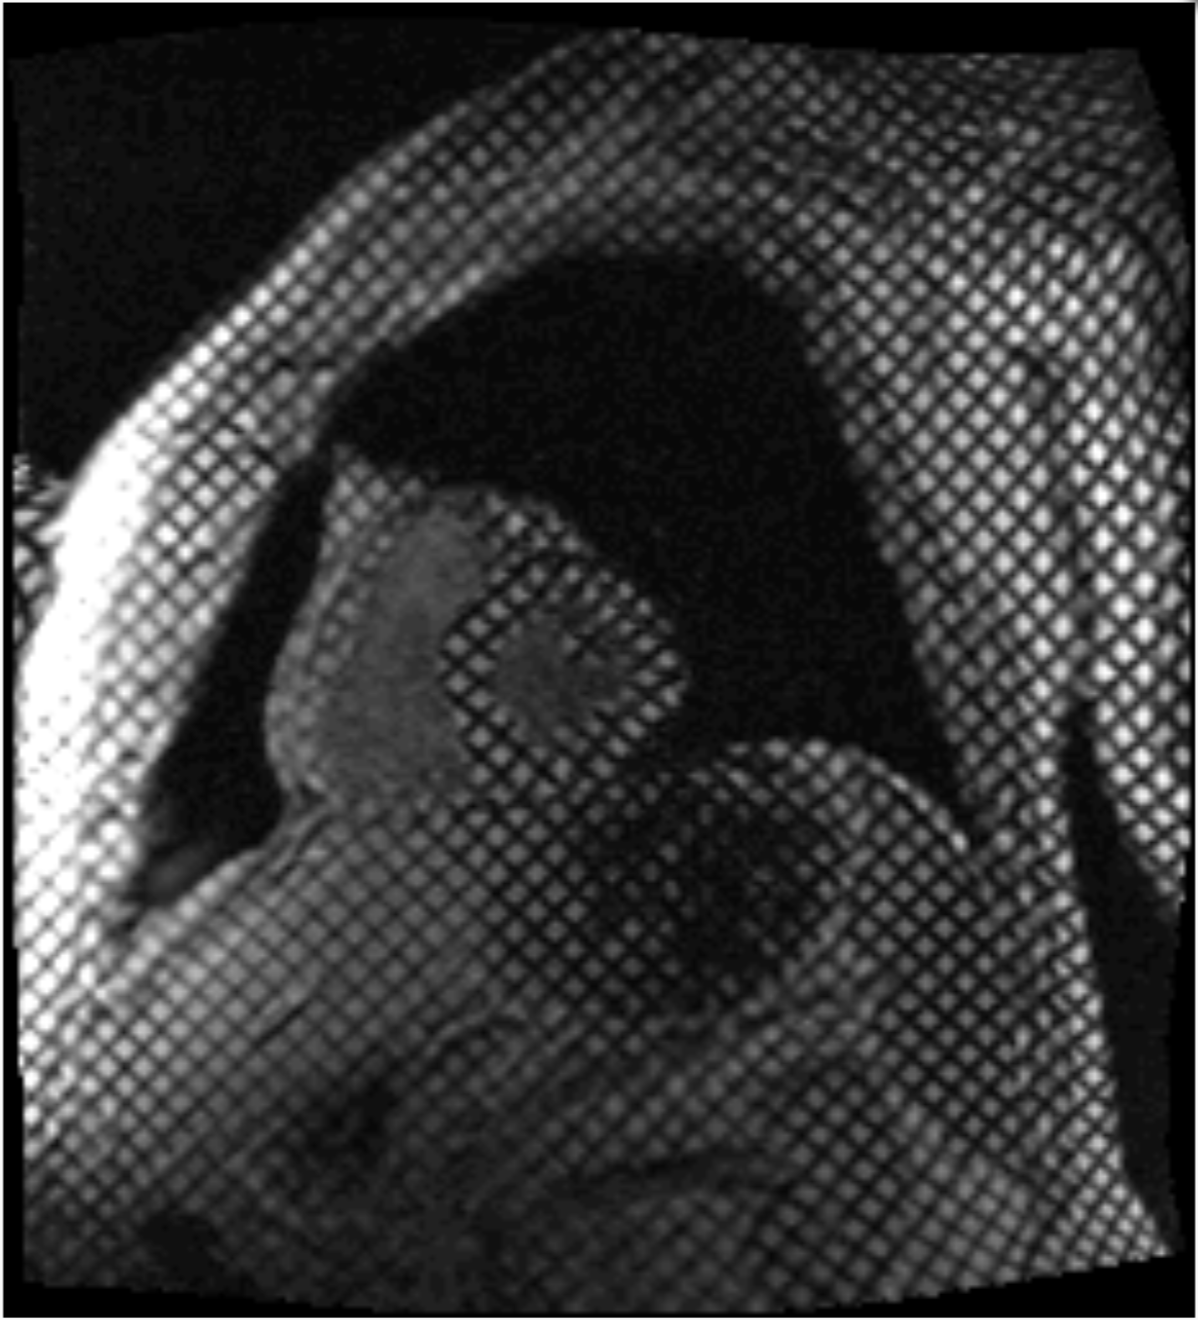
\includegraphics[height=6cm]{media/heart/tagged_heart.png}
        \captionsetup{justification=centering}
        \captionof{figure}[Tagovaná snímka myokardu pomocou techniky SPAMM]{Otagovaná snímka myokardu pomocou techniky SPAMM \cite{spamm_description}.}
\end {figure}

V súčasnej praxi sa SPAMM technika používa v situáciách, kde informácia o kontrakcii myokardu je kľúčová, ako napr. podozrenie na ischemickú chorobu srdca alebo na abnormality týkajúce sa neprirodzeného pohybu stien myokardu \cite{spamm_description} (vlastný preklad).

Nevýhodou použitia tejto techniky je skutočnosť, že táto mriežka sa stráca s blížiacim sa koncom srdcového cyklu. Samotné čiary mriežky sa pri konci systoly (časť srdcového cyklu, počas ktorej sa komory srdca sťahujú po naplnení krvou) môžu zlúčiť alebo úplne vyblednúť, čo sťažuje následnú analýzu pohybu srdca \cite{spamm_description} (vlastný preklad).

\begin {figure}[H]
        \centering
        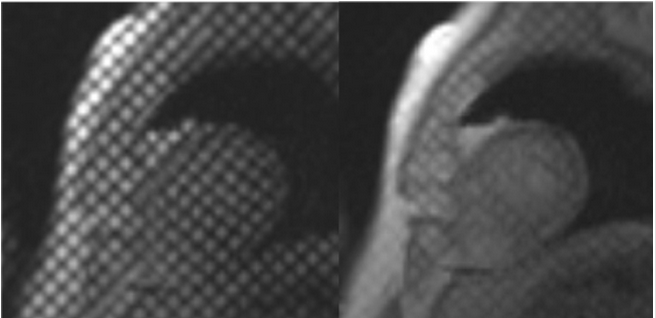
\includegraphics[height=6cm]{media/heart/early_late_systole.png}
        \captionsetup{justification=centering}
        \captionof{figure}[Ukážka vyblednutia SPAMM mriežky]{Ľavý obrázok zobrazuje začiatok systoly, pravý jej koniec.}
\end {figure}

\clearpage
        \chapter {Analýza súčasnej aplikácie}
Táto kapitola sa zaoberá účelom súčasnej aplikácie a analýzou použitých technológií, ktoré boli použité pri vývoji súčasnej aplikácie. Následne sú popísané podprogramy, ktoré riešia výpočtovo náročnejšie úlohy v rámci aplikácie. Jednému z najdôležitejších podprogramov -- \texttt{grid-tracker} -- je venovaná väčšia pozornosť. Ďalej je venovaná pozornosť zostaveniu a spusteniu aplikácie,\newline bez ktorej by nebolo možné prejsť k analýze používateľského rozhrania. \newline Posledná sekcia tejto kapitoly prináša postrehy z testovania aplikácie a popis problémov s ňou spojených.

\section {Účel aplikácie}
Účelom súčasnej aplikácie -- DICOM Viewer -- je analýza pohybu srdcového svalu, pomocou ktorej by bolo možné zistiť anomálie v jeho pohybe. Aplikácia umožňuje importovať súbory typu DICOM (popísaného v sekcii \ref{dicom}) obsahujúce snímky z magnetickej rezonancie, ktoré sú otagované SPAMM mriežkou.

Na importovaných snímkach môže používateľ vytvoriť mriežku, ktorej parametre môžu byť manuálne upravené. Táto mriežka by mala kopírovať mriežku vytvorenú SPAMM technikou. Štruktúra a parametre týchto mriežok sú neskôr spracované podprogramom \texttt{grid-tracker}, ktorého úlohou je zarovnanie používateľom vytvorených mriežok s mriežkami vytvorenými SPAMM technikou.

\clearpage
Po ich zarovnaní by malo byť možné pomocou techniky grafových rezov odsegmentovať srdečné komory a tým pádom zúžiť analýzu pohybu srdcového svalu len na tieto komory.

\section {Použité technológie}
Táto sekcia sa venuje popisu použitých technológií v súčasnej desktopovej aplikácii. Na základe zistenia, aké technológie a aplikačné závislosti aplikácia využíva, bude možné aplikáciu zostaviť a vyskúšať.

Nasledujúci prehľad použitých technológií je založený na dôslednom preskúmaní zdrojového kódu aplikácie, ktorý sa vyznačoval skoro neexistujúcou dokumentáciou.

\subsection {DICOM}\label{dicom}
V súčasnosti sú snímky získané pomocou zobrazovacích techník v medicíne zväčša ukladané v archivačnom a komunikačnom systéme snímkov. Tento systém ukladá nielen snímkové dáta, ale aj iné relevantné dáta podľa štandardu známym pod skratkou DICOM\footnote{https://www.dicomstandard.org} (Digital Imaging and Communications in Medicine) \cite{Varma_2012} (vlastný preklad).

DICOM je medzinárodným štandardom pre komunikáciu a manažment informácií o medicínskych obrazových a k nim príslušných dátach. Definuje, ako majú byť takéto dáta spracovávané, ukladané, tlačené a prenášané medzi zariadeniami podporujúcimi príjem týchto dát \cite{about_dicomlibrary} (vlastný preklad).

Začiatok vývoja DICOM štandardu sa datuje k prelomu 80. a 90. rokoch 20. storočia, kedy započala spolupráca medzi American College of Radiology a National Electrical Manufacturers Association. NEMA taktiež vlastní autorské práva k tomuto štandadu. Momentálne sa DICOM skladá z 22 nezávislých častí, z ktorých avšak nie všetky musia byť implementované zariadením podporujúcim tento štandard \cite{dicom_history} (vlastný preklad).

\clearpage

Pre účely spracovania snímkových dát, DICOM štandard vo svojej 10. časti definuje dátovú štruktúru (formát) súboru, do ktorého sa tieto dáta ukladajú. Súbor, ktorý spĺňa podmienky 10. časti tohto štandardu, býva značený ako \uv{DICOM Part 10} súbor, inak známy ako DICOM súbor \cite{Varma_2012} (vlastný preklad).

Štruktúra tohto (binárneho) súboru je nasledovná -- prvých 128 bajtov býva zväčša prázdnych (vyplnených 0). Ďalšie 4 bajty obsahujú reťazec \uv{DICM}.\newline Na základe týchto bajtov sa dá určiť, či sa jedná alebo nejedná o DICOM súbor. Ďalej nasleduje hlavička, ktorá je rozdelená na viacero skupín zoskupujúcich súvisiace atribúty. Konkrétne atribúty sa adresujú tagom - ten sa skladá z 8 čísiel v hexadecimálnom formáte. Prvé 4 čísla reprezentujú skupinu, v ktorej sa daný atribút nachádza. Posledné 4 čísla jednoznačne identifikujú konkrétny atribút v skupine \cite{Varma_2012} (vlastný preklad).

Ako príklad je uvedené získanie informácie o pacientovom veku - všetky informácie o pacientovi sa nachádzajú v skupine 0010. Pacientov vek v tejto skupine sa nachádza na pozícii 1010, tým pádom výsledný tag, pod ktorým nájdeme vek pacienta je (0010, 1010). Ku každému tagu je jednoznačne priradená reprezentácia jej hodnoty, ktorý určuje dátový typ, formát a dĺžku hodnoty daného atribútu  \cite{Varma_2012} (vlastný preklad).

Po hlavičke nasleduje skupina 7FE0, ktorá už obsahuje dáta o samotných obrazových pixeloch \cite{Varma_2012} (vlastný preklad). Typ kódovania týchto dát určuje Transfer Syntax -- ten udáva, akým spôsobom sú obrazové pixely zakódované. Transfer Syntax obsahuje taktiež informáciu, v akom poradí bajtov sú informácie zakódované (Little Endian vs Big Endian) a aká kompresia obrazových dát bola použitá \cite{dicom_transfer_syntax} (vlastný preklad).

\subsection {Qt}
Súčasná aplikácia bola vyvinutá pomocou Qt\footnote{https://www.qt.io/product/qt6} -- cross-platformového frameworku určeného pre vytváranie aplikácií najmä v jazyku C\texttt{++}\footnote{https://isocpp.org}. Aplikácie vyvinuté týmto frameworkom majú výhodu v tom, že sú spustiteľné na rôznych operačných systémoch s minimálnym počtom zmien v zdrojovom kóde \cite{qt_description} (vlastný preklad).

V súčasnosti (od roku 2014) zastrešuje vývoj tohto frameworku spoločnosť The Qt Company.

Výsadou Qt frameworku je rozdelenie jeho funkcionality do jednotlivých modulov. Pri následnom vývoji aplikácie sa použijú len tie moduly, ktoré \newline sú v danej aplikácii potrebné \cite{qt_description} (vlastný preklad).

Existujúca aplikácia využíva tento framework vo verzii 5.15, ktorá sa vyznačuje tým, že je verziou s dlhodobou podporou. Koniec podpory tejto verzie je naplánovaný na koniec mája 2023. Najnovšou verziou Qt frameworku je momentálne verzia 6.5, ktorá je taktiež verziou s dlhodobou podporou.

V súčasnej aplikácii sa používajú nasledovné moduly: 
\begin{itemize}
\item {Qt Core,}
\item {Qt Widgets,}
\item {Qt GUI a}
\item {Qt Test.}
\end{itemize}

Qt Core modul obsahuje najpoužívanejšie triedy ako napr. \texttt{QCoreApplication}, \texttt{QObject}, \texttt{QDebug} a iné. Nakoľko sú tieto triedy používané aj inými modulmi, je tento modul implicitne nalinkovaný Qt frameworkom pri budovaní aplikácie \cite{qtcore_description} (vlastný preklad).

Qt Widgets modul poskytuje UI elementy, ktoré sú určené pre vytváranie používateľského rozhrania. Tieto elementy môžu zobrazovať rozličné dáta, prijímať vstup z klávesnice, byť štylizované a zoskupované do rozličných usporiadaní \cite{qtwidgets_description} (vlastný preklad). Existujúca aplikácia používa z modulu napr. triedu \texttt{QMainWindow}, ktorá je zodpovedná za vykreslenie aplikačného okna a taktiež triedu \texttt{QGraphicsScene}, ktorá je zodpovedná za vykreslenie snímkov z magnetickej rezonancie v DICOM formáte.

\clearpage

Qt GUI modul obsahuje triedy určené pre zobrazovanie aplikačného okna a iného grafického obsahu s následnou obsluhou udalostí. Taktiež obsahuje triedy, ktoré sú zodpovedné za zobrazovanie 2D grafiky, fontov a typografie \cite{qtgui_description} (vlastný preklad).
Súčasná aplikácia z tohto modulu používa napr. triedu \texttt{QImage}, ktorá obsahuje metódy pre priamy prístup k pixelom snímkov a ich manipuláciu.

Qt Test modul poskytuje rozličné triedy pre jednotkové testovanie Qt aplikácií a príslušných knižníc \cite{qttest_description} (vlastný preklad) -- v súčasnej aplikácii bol tento modul využitý pri testovaní grafického používateľského rozhrania a funkcionalít súčasnej aplikácie, ako napr. testovanie zmien v nastaveniach vykreslenej mriežky na obrázku z magnetickej rezonancie.

\subsection {Qmake}\label{qmake}
Pre zjednodušenie písania Makefilov, ktoré definujú, ako má byť program skompilovaný, bol použitý nástroj Qmake\footnote{https://doc.qt.io/qt-5/qmake-manual.html}. Tento nástroj pochádza taktiež z dielne The Qt Company.

Qmake umožňuje vývojárom definovať vytvorenie Makefilu pomocou syntaxe definovaného programom Qmake \cite{qmake_description} (vlastný preklad). Výsledkom tohto procesu je \texttt{.pro} súbor obsahujúci inštrukcie, ako daný Makefile vytvoriť. \newline Následne sa pomocou príkazu \texttt{qmake} s argumentom cesty k \texttt{.pro} súboru vytvorí \texttt{Makefile} súbor, pomocou ktorého je možné daný program skompilovať, čoho výsledkom je spustiteľný súbor aplikácie.

Pre súčasnú aplikáciu sa daný súbor volá \texttt{Cameo.pro} a nachádza sa v adresári \texttt{dicomViewer}.

\clearpage

\subsection {DCMTK}\label{dcmtk}
DCMTK je knižnica, ktorá implementuje veľkú časť DICOM štandardu\newline v jazykoch C a C\texttt{++}. Úlohou tejto knižnice je okrem skúmania DICOM súborov aj ich vytváranie a konverzia, manipulácia s pamäťovými médiami a odosielanie, či prijímanie obrazových súborov cez internetové pripojenie \cite{dcmtk_description} (vlastný preklad).

Za jej vývojom stojí nemecká firma OFFIS, ktorá túto knižnicu vyvíja od roku 1993. V súčasnosti sa DCMTK knižnica používa v nemocniciach a rôznych spoločnostiach po celom svete, kde predstavuje softvérový základ pri rozličných výskumných projektoch, prototypoch a komerčných produktoch nevynímajúc \cite{dcmtk_description} (vlastný preklad).

Súčasná aplikácia je kompatibilná s najnovšou verziou tejto knižnice, ktorou je verzia 3.6.7. DCMTK knižnica je v tejto aplikácii použitá pre získanie informácií z hlavičiek DICOM súborov, ako napr:
\begin{itemize}
\item {údaje o pacientovi,}
\item {údaje o snímke a}
\item {údaje o sérií snímkov.}
\end{itemize}

\subsection {OpenMP}\label{openmp}
OpenMP\footnote{https://www.openmp.org} poskytuje rozhranie pre programovanie aplikácií (tzv. API), vďaka ktorému je možné vytvárať C\footnote{https://www.open-std.org/jtc1/sc22/wg14/}, C\texttt{++} a Fortran\footnote{https://fortran-lang.org/en/} aplikácie využívajúce viac vlákien nad zdieľanou pamäťou \cite{openmp_description}.

Vývoj OpenMP v súčasnosti zastrešuje OpenMP Architecture Review Board \cite{openmp_description}.

\clearpage
OpenMP funguje na báze direktív, pomocou ktorých sa jednotlivé časti programu dajú paralelizovať viacerými spôsobmi -- a to paralelizáciou prevádzania jednotlivých úloh (tzv. funkčný paralelizmus -- vhodný pre paralelizáciu rekurzívnych algoritmov, kde úloha $\equiv{ volanie funkcie}$) alebo paralelizáciou dátovo nezávislých iterácií (tu sa jedná o tzv. iteračný dátový paralelizmus) \cite{openmp_description}.

Existujúca aplikácia využíva direktívy OpenMP pre paralelizáciu výpočtovo náročnejších algoritmov. Súčasná verzia OpenMP, verzia 5.2, je plne kompatibilná s aktuálnym zdrojovým kódom aplikácie.

\subsection {TNL}\label{tnl}
Template Numerical Library\footnote{https://tnl-project.org} je numerická knižnica, ktorá poskytuje rozličné dátové štruktúry, ktoré uľahčujú prácu s pamäťou a vývoj efektívnych numerických riešičov. Táto knižnica je implementovaná pomocou C\texttt{++} s cieľom poskytnúť flexibilné a užívateľsky prívetivé rozhranie. TNL poskytuje natívnu podporu pre moderné hardwarové architektúry ako sú viacjadrové CPU, GPU a distribuované systémy, ktoré je možné spravovať cez jednotné rozhranie \cite{tnl_description}.

Vývoj TNL knižnice od jej počiatku riadi Tomáš Oberhuber z Katedry matematiky na FJFI ČVUT v spolupráci s Jakubom Klinkovským a Alešom Wodeckim.

V súčasnej aplikácii sú z TNL knižnice použité kolekcie ako napr. \texttt{String} pre manipuláciu s reťazcami a \texttt{Containers::Array}, \texttt{Containers::\{Vector,\newline StaticVector,MultiVector\}}, čo sú šablóny pre reprezentáciu \newline n-dimenzionálnych polí, ktoré abstrahujú manažment dát a spúšťanie bežných operácií na rozličných hardvérových architektúrach.

Aplikácia z TNL knižnice taktiež používa \texttt{Solvers::ODE::Merson} -- jedná sa o riešič používajúci Runge-Kutta-Merson metódu štvrtého rádu s adaptívnym výberom časového kroku, vďaka ktorému je možné získať približné riešenie diferenciálnych rovníc.

\clearpage

Bohužiaľ, súčasná aplikácia nie je kompatibilná s najnovšími zdrojovými kódmi TNL knižnice -- pre nájdenie posledného \uv{dobrého stavu} knižnice, t.j. stavu za ktorého bolo možné aplikáciu skompilovať, bol využitý nástroj \texttt{git bisect}. Tento nástroj našiel ako posledný \uv{dobrý stav} knižnice z 13.5.2021. Pri využití TNL knižnice zostavenej po tomto dátume nebolo možné súčasnú aplikáciu skompilovať.

\section {Pomocné podprogramy}\label{helper_apps}
Súčasná aplikácia obsahuje a využíva nasledujúce 3 podprogramy:

\begin {itemize}
\item {grid-tracker,}
\item {local-variance a}
\item {graph-cuts.}
\end {itemize}

Prvý z týchto podprogramov -- \texttt{grid-tracker} -- je C\texttt{++} podprogram určený pre sledovanie pohybu myokardu pomocou detekcie SPAMM mriežky\newline z DICOM snímky a mriežky vytvorenej používateľom. Mriežku vytvorenú používateľom sa snaží zarovnať so SPAMM mriežkou pre každú snímku zo sekvencie snímkov.

Vstupom tohto programu sú nasledujúce parametre:
\begin {itemize}
\item {\texttt{inputImageFileNames} -- vektor reťazcov reprezentujúci cesty k súborom multivectorov (definované TNL knižnicou), ktoré obsahujú enkódované DICOM snímky,}
\item {\texttt{inputGridFileNames} -- vektor reťazcov reprezentujúci cesty k súborom používateľom definovaných mriežok uložených ako TNL textový multivector,}
\item {\texttt{outputGridFileNames} (nepovinné) -- vektor reťazcov reprezentujúce cesty k súborom spracovaných mriežok, ktoré budú uložené ako textový TNL multivector,}
\item {\texttt{curvatureCoefficient} -- závislosť vývoja mriežky od zakrivenia, vyššie číslo znamená vyššiu závislosť,}
\item {\texttt{forceCoefficient} -- závislosť mriežky od gradientu obrazu, vyššie číslo znamená vyššiu závislosť a}
\item {\texttt{stopTime} -- časový interval algoritmického výpočtu.}
\end {itemize}

Pre daný výpočet \texttt{grid-tracker} využíva technológie \nameref{tnl} a \nameref{openmp}.

Jeho výstupom by mali byť predchádzajúce používateľom definované mriežky v textovom TNL multivektore upravené algoritmom tak, aby mriežky zodpovedali mriežkam definovanými SPAMM metódou.

Nasledujúce dva C\texttt{++} podprogramy nie sú dôležité pre túto diplomovú prácu, avšak pre úplnosť je ich účel vysvetlený.

Úlohou \texttt{local-variance} podprogramu je aplikovanie filtra lokálnej variancie na danú snímku za účelom lepšej segmentácie srdcových komôr. Tento filter je implementovaný pomocou jednoduchého rozptylového filtru, ktorý vypočíta priemernú intenzitu pixelov vo štvorcovom okolí každého pixelu a túto hodnotu dosadí do výberového rozptylu, ktorý sa bude rovnať novej hodnote intenzity pixelu \cite{master_thesis_app}.

Podprogram \texttt{graph-cuts} slúži pre segmentáciu srdcových komôr, ktorý vychádza z predpokladu, že hranica medzi objektom a jeho pozadím sa nachádza v miestach nekonzistencie susedných pixelov snímky. Implementovaná metóda, ktorá dosiahla dobré výsledky segmentácie, je metóda grafových rezov, kombinujúca Fordov-Fulkersonovým algoritmom s Preflow-Push algoritmom \cite{master_thesis_app}.

\section {Zostavenie aplikácie a jej spustenie}
Pre potrebu popísania používateľského rozhrania je najprv žiaduce dosiahnuť zostavenie existujúcej aplikácie a jej následné spustenie. Po počiatočnej analýze zdrojového kódu, v ktorom bolo zistené, že aplikácia bola vyvíjaná pre Linuxové prostredie, bol vo virtuálnom prostredí nainštalovaný operačný systém Ubuntu 22.10\footnote{https://ubuntu.com}.

Pre zostavenie súčasnej aplikácie je potrebné nainštalovať Qt framework spolu s nástrojom Qmake, nakoľko ich architektúra súčasnej aplikácia vyžaduje.

Inštalácia Qt frameworku a Qmake nástroja je možná pomocou inštalácie balíčka \texttt{qt5-default}\footnote{sudo apt install qt5-default}. Ten okrem iného obsahuje aplikáciu Qt Creator\footnote{https://doc.qt.io/qtcreator/}.

Qt Creator je aplikácia, ktorá poskytuje prostredie pre integrovaný vývoj aplikácií postavených nad Qt frameworkom. Pomocou tejto aplikácie je možné vyvíjať, testovať, zostavovať, spúšťať a debugovať aplikácie postavené na tomto frameworku.

Okrem balíčku \texttt{qt5-default} je taktiež potrebné nainštalovať balíčky \texttt{cmake}\footnote{sudo apt install cmake} a \texttt{build-essential}\footnote{sudo apt install build-essential}, čo sú balíčky poskytujúce ďalšie nástroje potrebné\newline pre zostavenie aplikácie. Tieto balíčky už môžu byť súčasťou použitej linuxovej distribúcie, čo ale neplatilo v prípade použitia Ubuntu 22.10 ako operačného systému.

Nakoľko súčasná aplikácia využíva DCMTK knižnicu, ako bolo popísané\newline v sekcii \ref{dcmtk}, je taktiež nutné nainštalovať nasledujúce balíčky: \texttt{dcmtk}\footnote{sudo apt install dcmtk} \newline a {\texttt{libdcmtk-dev}\footnote{sudo apt install libdcmtk-dev}.

Prvý z uvedených balíčkov nainštaluje samotnú DCMTK knižnicu, druhý obsahuje knižnice a hlavičkové súbory pre vývoj aplikácií používajúce túto knižnicu. Nakoľko sa v \texttt{Dicom.pro} súbore (ktorý je určený pre výsledné zostavenie aplikácie) nachádzajú cesty ku knižniciam z balíčku \texttt{libdcmtk-dev}, je aj tento balíček nutný nainštalovať pre neskoršie korektné spustenie súčasnej aplikácie.

Keďže \texttt{grid-tracker} podprogram obsahuje OpenMP direktívy pre paralelizáciu výpočtových algoritmov, je potrebné nainštalovať OpenMP prostredníctvom balíčku \texttt{libomp-dev}\footnote{sudo apt install libomp-dev}.

\clearpage
TNL knižnica bude taktiež benefitovať z inštalácie tohto balíčka, nakoľko sama využíva OpenMP pre paralelizáciu algoritmov, čo znamená, že je potrebné tento balíček nainštalovať ešte pred samotnou inštaláciou TNL knižnice.

Ďalej je potrebné nainštalovať TNL knižnicu -- pre jej inštaláciu je potrebné stiahnuť zdrojové kódy buď formou zabaleného zdrojového kódu v .zip balíčku, alebo naklonovaním repozitára pomocou programu \texttt{git}\footnote{https://git-scm.com}. Keďže aplikácia je nekompatibilná s najnovšou verziou TNL knižnice, je potrebné stiahnuť alebo naklonovať repozitár so zdrojovými kódmi do dátumu 13.5.2021 (viď \ref{tnl}).

Pretože je nutné samotnú knižnicu zo zdrojových kódov zostaviť, je nevyhnutné mať nainštalovaný kompilátor podporovaný samotnou knižnicou.

Medzi podporované kompilátory sa radí GCC\footnote{http://gcc.gnu.org} kompilátor vo verzii 8.0\newline a vyššie alebo Clang\footnote{https://clang.llvm.org} vo verzii 7.0 a vyššie. Prvý z nich je možné nainštalovať pomocou balíčku \texttt{gcc}\footnote{sudo apt install gcc} a druhý pomocou balíčku \texttt{clang}\footnote{sudo apt install clang}.

Následne je potrebné spustiť inštalačný skript \texttt{install}, ktorého účelom je nakonfigurovanie TNL knižnice a jej zostavenia.
Pred spustením samotného inštalačného skriptu \texttt{install} je potrebné zistiť, či sú nainštalované balíčky \texttt{doxygen}\footnote{https://doxygen.nl/index.html}, \texttt{matplotlib}\footnote{https://matplotlib.org} a \texttt{graphviz}\footnote{https://graphviz.org}.

Tieto balíčky sa využívajú pri generovaní dokumentácie počas spustenia \texttt{install} skriptu (pri defaultnej inštalácii). Ak sa niektorý z daných balíčkov nenachádza v systéme, je potrebné ho doinštalovať.

Po nainštalovaní všetkých potrebných balíčkov sa TNL knižnica zostaví spustením \texttt{install}\footnote{chmod +x install \&\& ./install} skriptu. Po jeho ukončení sa hlavičkové súbory TNL knižnice nachádzajú v priečinku \texttt{/usr/lib/aarch64-linux-gnu}.

\clearpage
Názov posledného priečinku sa môže líšiť, nakoľko je závislý na architektúre CPU, na ktorom sa TNL knižnica zostavuje. V tomto prípade bola knižnica zostavovaná na systéme Ubuntu 22.10 bežiacom nad CPU s architektúrou Aarch64 (Apple M1 Pro CPU).

Ďalším krokom pre úspešné zostavenie aplikácie je definovanie cesty k hlavičkovým súborom TNL knižnice v samotnom \texttt{Cameo.pro} súbore. Po otvorení súboru \texttt{Cameo.pro} je potrebné nastaviť hodnotu premennej \lstinline{DCMTK_LIBS} -- tá obsahuje cesty k DCMTK knižniciam, ktoré súčasná aplikácia využíva.\newline V tomto prípade ju bolo potrebné nastaviť na horeuvedený priečinok \newline \texttt{/usr/lib/aarch64-linux-gnu} a následne daný súbor uložiť.

Po prevedení všetkých predchádzajúcich krokov je možné spustiť nástroj \texttt{qmake} pomocou krokov popísaných v sekcii \ref{qmake}.\newline Jeho výsledkom je \texttt{Makefile} súbor, ktorý definuje kroky, ako zostaviť súčasnú aplikáciu. V tomto momente je už možné súčasnú aplikáciu skompilovať pomocou príkazu \texttt{make install}.

Po skompilovaní aplikácie sa v rovnakom priečinku objaví spustiteľný súbor \texttt{Cameo}, ktorému je potrebné nastaviť práva pre spustenie príkazom \texttt{chmod +x Cameo}. Následne je možné spustiť aplikáciu príkazom \texttt{./Cameo}. \clearpage

\section {Používateľské rozhranie}\label{old_ui}
Po úspešnom spustení aplikácie sa používateľovi zobrazí jej hlavné okno, ktorého obsah je možné vidieť na nasledujúcom obrázku.
\begin {figure}[ht]
        \centering
        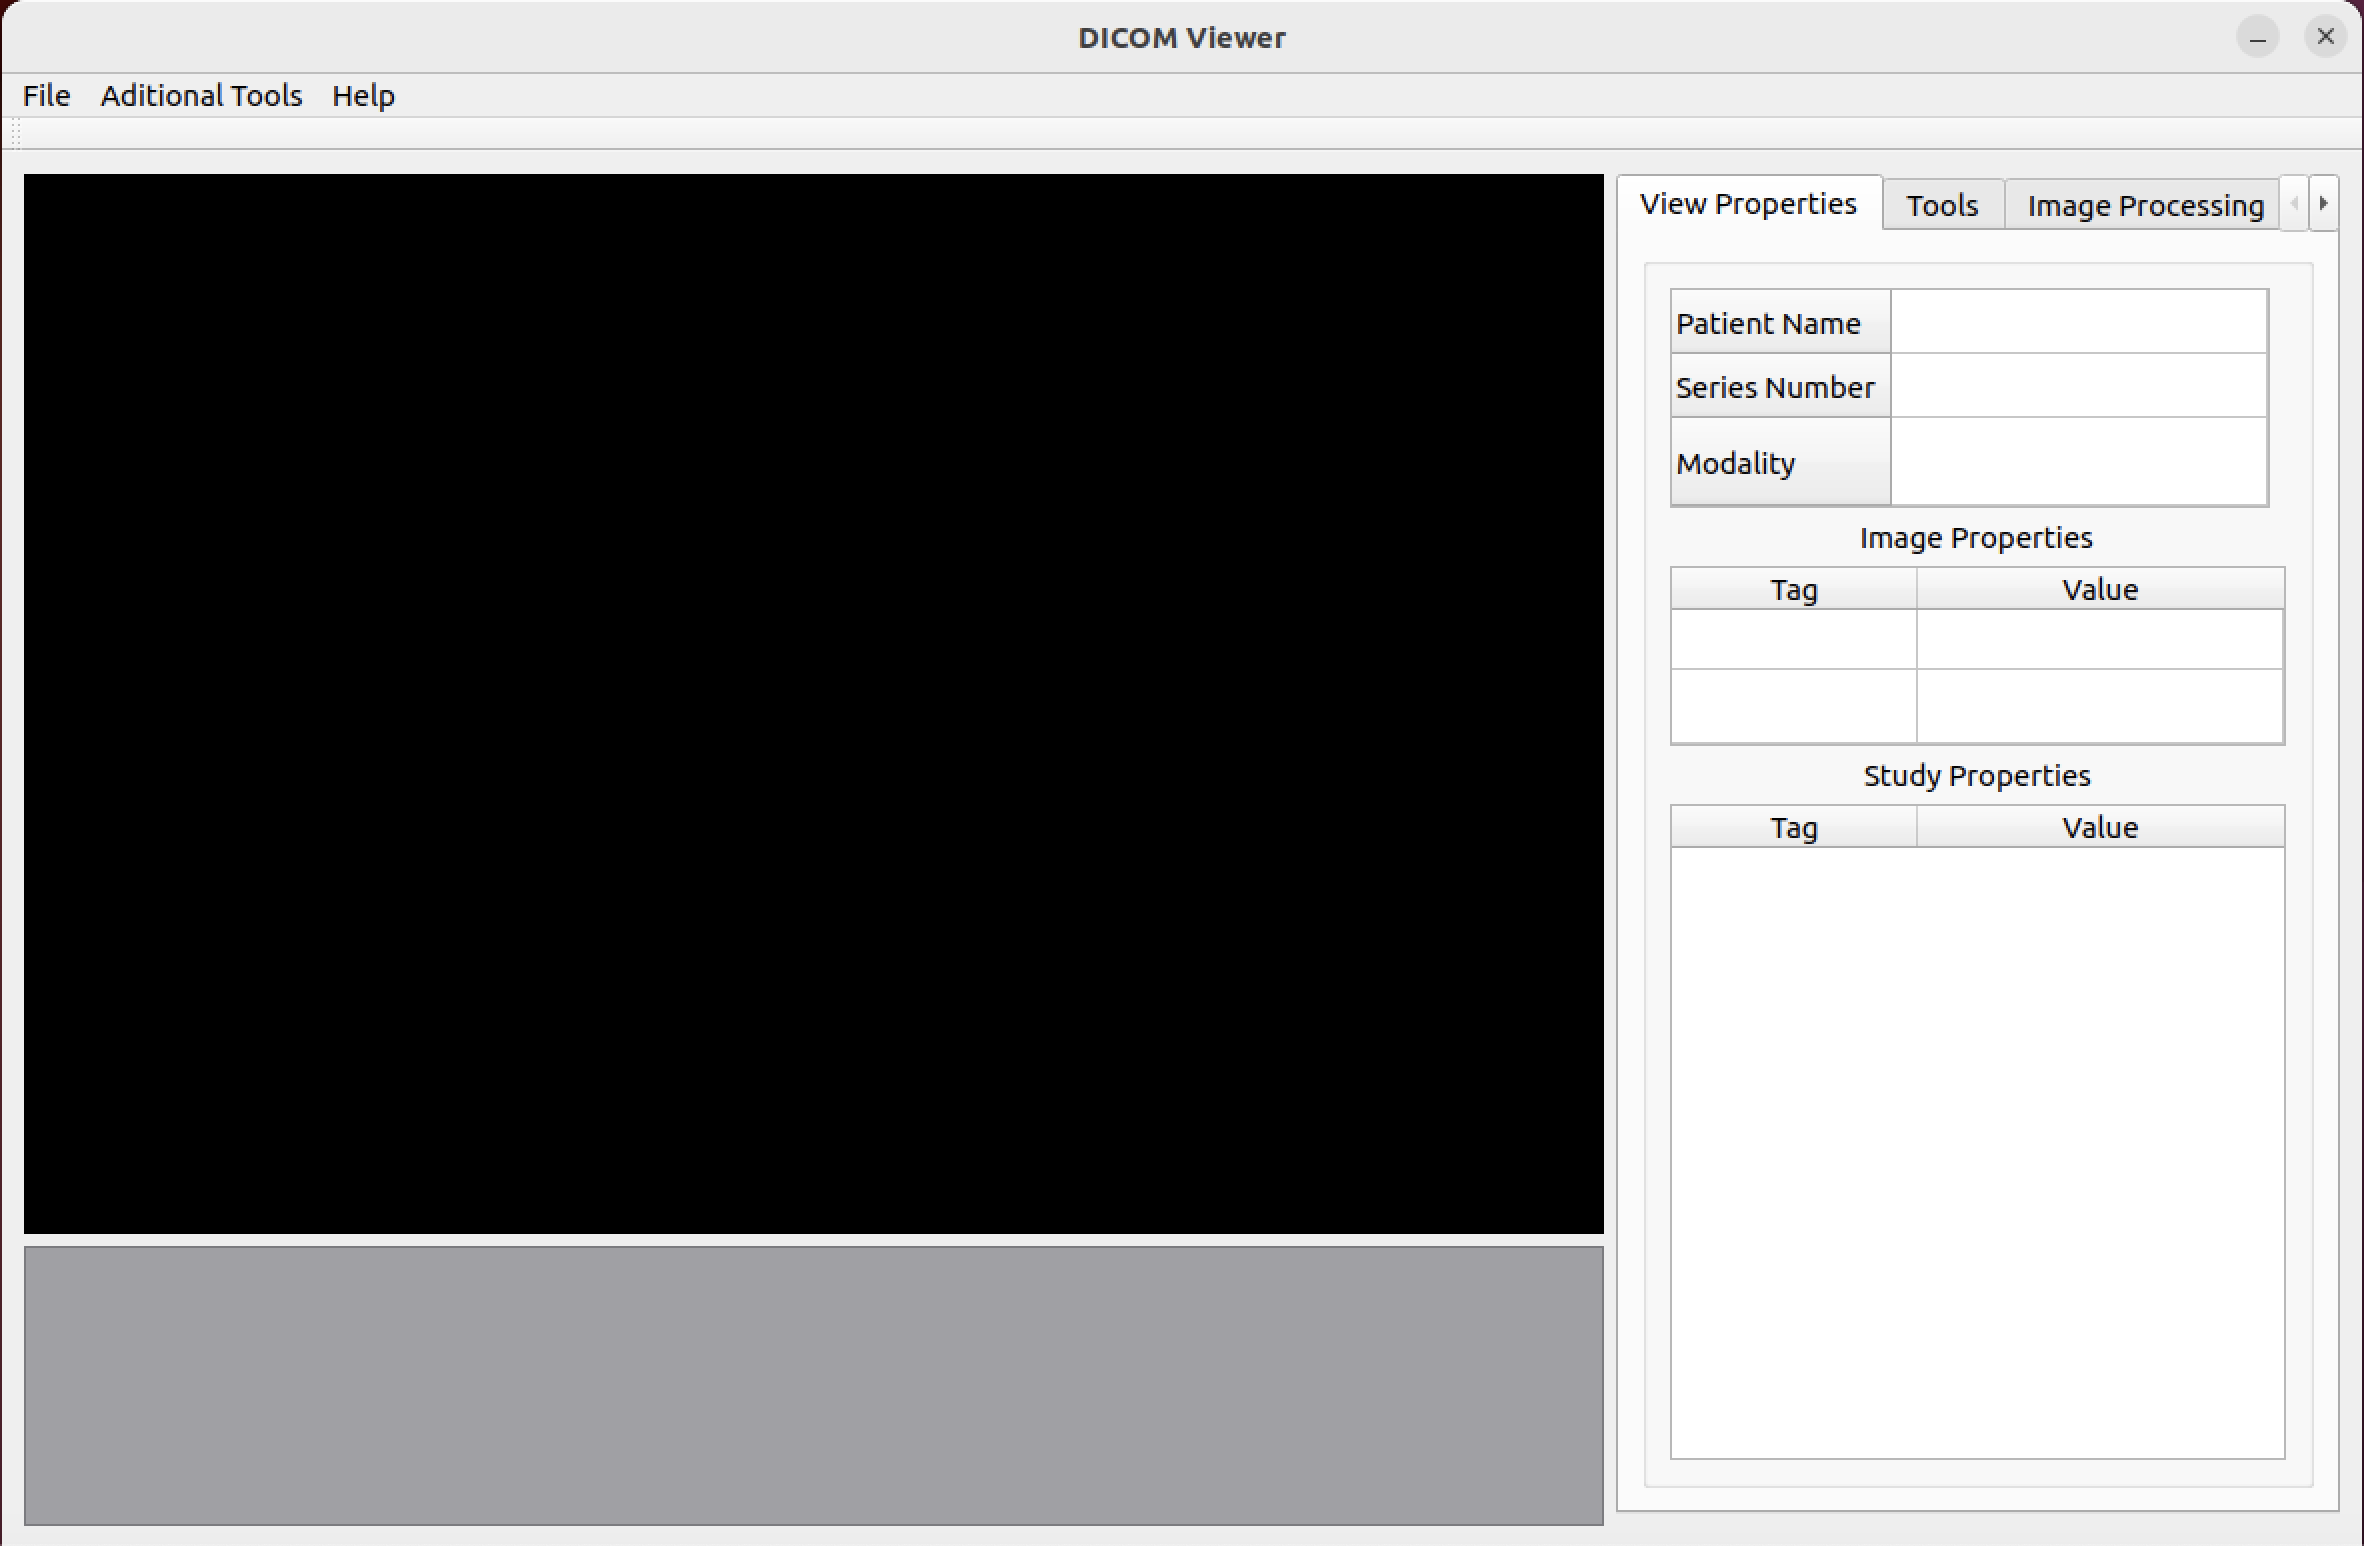
\includegraphics[height=8cm]{media/existing_app/init.png}
        \captionsetup{justification=centering}
        \captionof{figure}[Ukážka DICOM Viewer aplikácie po jej spustení]{Ukážka DICOM Viewer aplikácie po jej spustení}
\end {figure}

Používateľské rozhranie aplikácie je možné rozdeliť na nasledovné časti:
\begin {itemize}
\item {aplikačné menu,}
\item {ľavý postranný panel,}
\item {centrálnu časť aplikácie a}
\item {pravý postranný panel.}
\end {itemize}

Na zobrazenom obrázku nie je možné vidieť ľavý postranný panel, nakoľko ten je po spustení aplikácie predvolene skrytý.\clearpage

\subsection {Aplikačné menu}
V hornej časti okna aplikácie je zobrazené aplikačné menu. Toto menu pozostáva z troch hlavných možností, ktoré obsahujú viacero úrovní.

Jeho obsah je nasledovný:
\begin {enumerate}
\item {File}
	\begin {enumerate}
		\item {Open -- otvorí systémové okno pre výber priečinku s DICOM snímkami, ktoré sa majú importovať do aplikácie.}
		\item {Save Image}
		\begin {enumerate}
			\item {Save View -- uloží pohľad na aktuálnu snímku vo zvolenom formáte,}
			\item {Save Scene -- uloží scénu vo zvolenom formáte,}
			\item {Save Area of Interes [sic] -- uloží plochu záujmu vo zvolenom formáte.}
		\end {enumerate}
	\item {Save all selected}
		\begin {enumerate}
			\item {Save View -- uloží pohľad vybraných snímky vo zvolenom formáte,}
			\item {Save Scene -- uloží scénu vybraných snímkov vo zvolenom formáte,}
			\item {Save Area of Interes [sic] -- uloží plochu záujmu vybraných snímkov vo zvolenom formáte.}
		\end {enumerate}	
	\item {Exit -- ukončí aplikáciu.}
	\end {enumerate}
\item {Aditional [sic] Tools}
	\begin {enumerate}
	\item {Grid Tools -- otvorí ľavý postranný panel aplikácie s nastavením mriežky,}
	\item {Lvf Tools -- otvorí ľavý postranný panel aplikácie s nastavením filtra lokálnej variácie,}
	\item {Graph Cuts Tools -- otvorí ľavý postranný panel aplikácie s nastavením grafových rezov.}
	\end {enumerate}
\item {Help}
	\begin {enumerate}
	\item {About -- zobrazí informácie o DICOM Viewer aplikácii.}
	\end {enumerate}
\end {enumerate}

\clearpage
\subsection {Import DICOM snímiek}
Aplikácia sa po spustení nachádza v stave, v ktorom nie je možné s ňou interagovať. To je spôsobené tým, že do aplikácie je potrebné importovať aspoň jednu snímku v DICOM formáte.

Import snímiek je možné dosiahnuť zvolením možnosti File $\rightarrow{  Open}$ z aplikačného menu. Následne sa otvorí systémové okno pre výber priečinka s DICOM snímkami, ktoré sa majú zobraziť v aplikácii. Bohužiaľ nie je možné zvoliť snímky jednotlivo z priečinku, čoho dôsledkom je načítanie všetkých snímiek z vybraného priečinku do aplikácie. Po jeho zvolení sa v aplikácii zobrazí prvá importovaná snímka.

Po výbere ľubovoľnej možnosti, ktoré ponúka Aditional [sic] Tools menu, sa taktiež zobrazí ľavý postranný panel v aplikácii, ako je možné vidieť na nasledujúcej snímke aplikácie. V tomto prípade bola zvolená možnosť \uv{Grid Tools}.

\begin {figure}[ht]
        \centering
        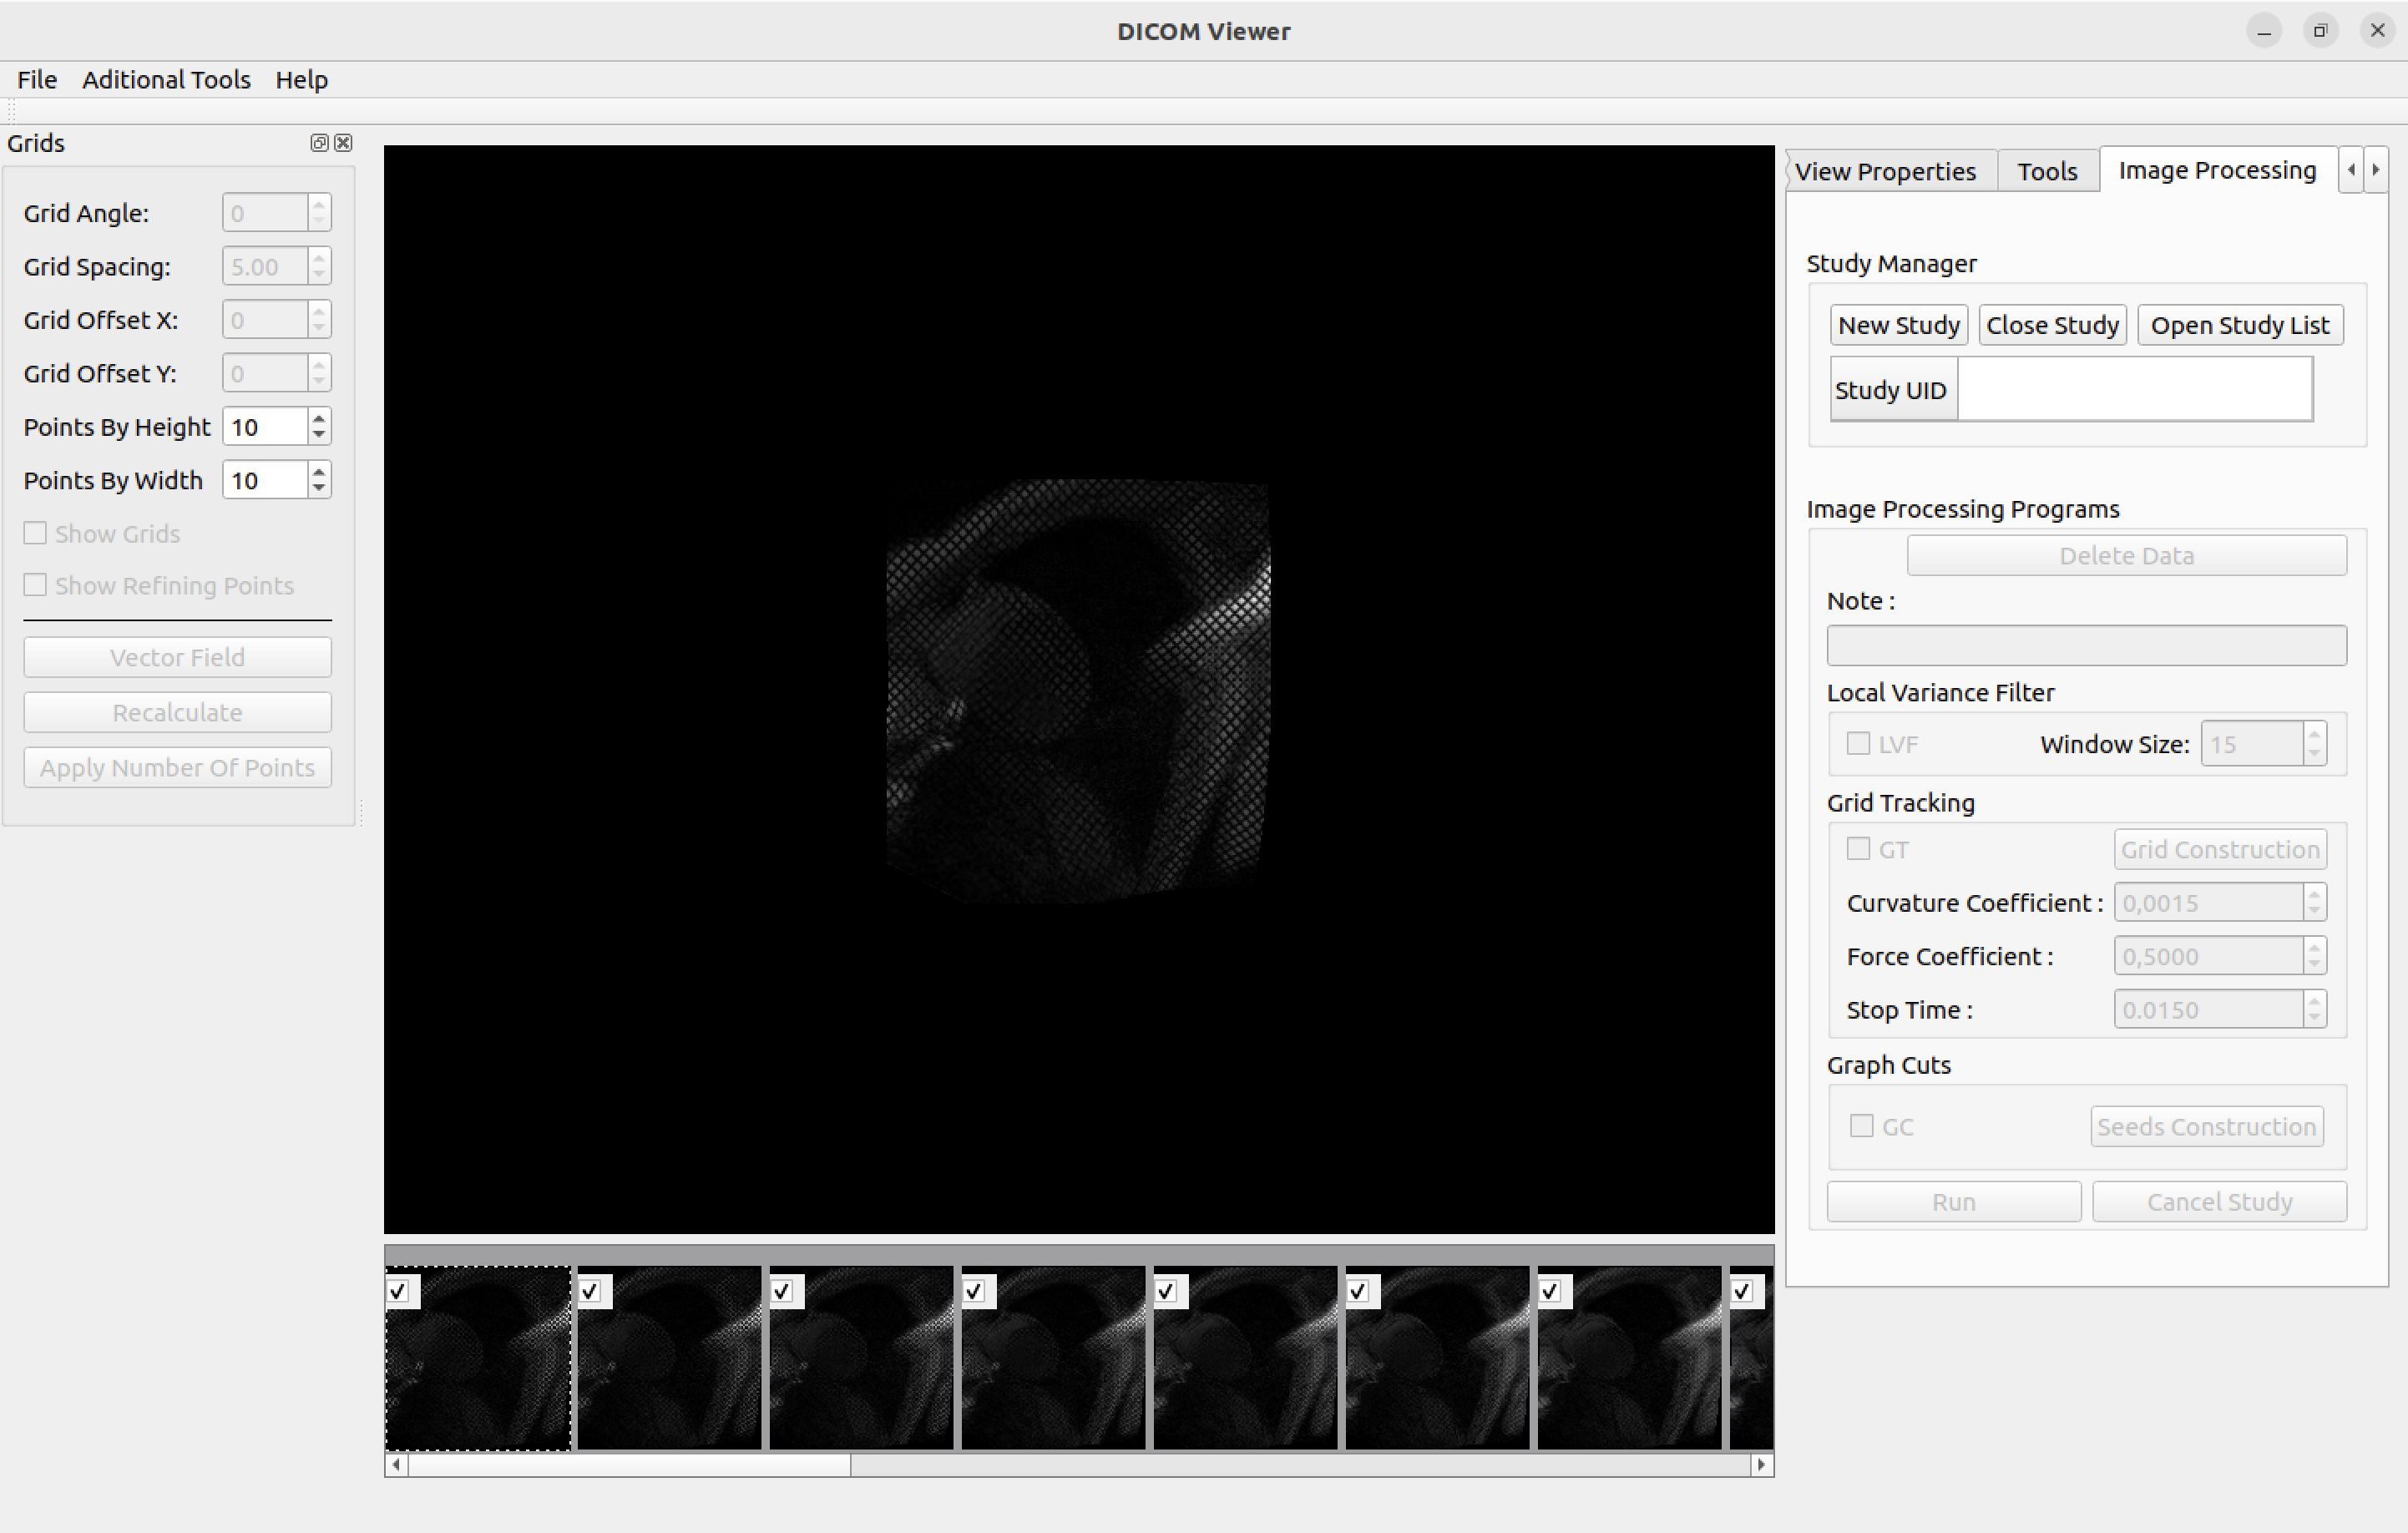
\includegraphics[height=8cm]{media/existing_app/app_with_grids_panel.png}
        \captionsetup{justification=centering}
        \captionof{figure}[Zobrazenie prvej snímky v DICOM Viewer aplikácii]{Zobrazenie prvej snímky v DICOM Viewer aplikácii}
\end {figure}

Zobrazením ľavého postranného panelu sa odhalí celková štruktúra používateľského rozhrania aplikácie.

\clearpage

\subsection {Ľavý postranný panel}\label{left_sidebar}
Obsah ľavého postranného panelu sa mení v závislosti na zvolenej možnosti\newline z menu Aditional [sic] Tools. Momentálne je na snímke zobrazený obsah ľavého panelu po zvolení možnosti \uv{Grid Tools}.

V ňom je možné nájsť nasledujúce možnosti:
\begin {itemize}
\item {Grid Angle -- uhol mriežky,}
\item {Grid Spacing -- rozpätie jednotlivých bodov,}
\item {Grid Offset X -- $x$ pozícia od ľavého horného bodu,}
\item {Grid Offset Y -- invertovaná $y$ pozícia od ľavého horného bodu,}
\item {Points by Height -- počet bodov na úsečku mriežky na výšku,}
\item {Points By Width -- počet bodov na úsečku mriežky na šírku,}
\item {Show Grids -- indikuje, či má byť zobrazená mriežka,}
\item {Show Refining Points -- indikuje, či majú byť zobrazené body, ktoré upresňujú pozíciu mriežky,}
\item {Vector Field -- spočíta rozdiel v pohybe mriežky medzi predchádzajúcou a aktuálnou snímkou,}
\item {Recalculate -- odošle dáta \texttt{grid-tracker} podprogramu pre opätovné zarovnanie mriežky voči SPAMM mriežke a}
\item {Apply Number of Points -- uloží mriežku ako textový TNL multivektor.}
\end {itemize}

Ostatné dve možnosti z menu \uv{Aditional [sic] Tools} nie je potrebné pre účely tejto práce popisovať.

\clearpage

\subsection {Centrálna plocha aplikácie}
Obsahom centrálnej plochy, ktorá je dominantná v zobrazení aplikácie, je aktuálne vybraná DICOM snímka. Nad ňou môže byť tiež vykreslená používateľom definovaná mriežka.

Pod touto plochou sú zobrazené náhľady všetkých snímiek, ktoré obsahujú zaškrtávacie políčko. Toto políčko reprezentuje možnosť, či má byť daná snímka spracovaná v rámci vybraného podprogramu.

\subsection {Pravý postranný panel}
Pravý postranný panel je rozdelený na nasledovné karty: \uv{View Properties}, \uv{Tools}, \uv{Image Processing} a \uv{History}.

\subsubsection {View Properties karta}
Karta \uv{View Properties} nie je interaktívna -- zobrazuje informácie ako meno pacienta nachádzajúceho sa na zobrazenej snímke, číslo série a modalitu snímiek. Taktiež je zobrazená výška a šírka aktuálne zobrazenej snímky.

\begin {figure}[H]
        \centering
        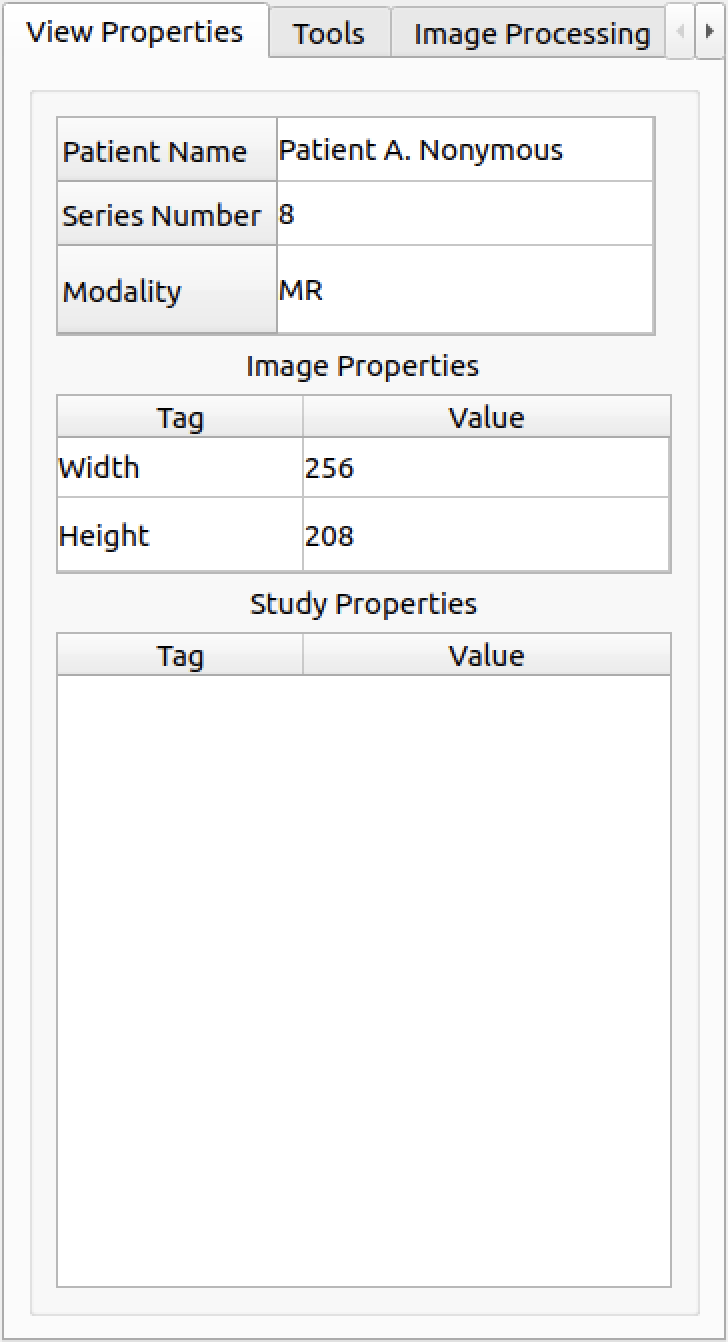
\includegraphics[height=8cm]{media/existing_app/tabs/view_properties.png}
        \captionsetup{justification=centering}
        \captionof{figure}{Zobrazenie obsahu kariet pravého postranného panelu}
\end {figure}

\clearpage

\subsubsection {Tools karta}
Na rozdiel od predchádzajúcej karty, \uv{Tools} karta obsahuje interaktívne prvky, ako napr. zobrazenie a zmena indexu zobrazenej snímky, či slider pre jej priblíženie. Snímke je taktiež možné zmeniť kontrast, jas a gammu pomocou sliderov.

Ďalej nasleduje sekcia pre nastavenie oblasti záujmu, pri ktorej je možné nastaviť jej zobrazenie alebo zmeniť jej výšku/šírku -- oblasť záujmu je na základe týchto nastavení vykreslená nad snímkou. 

Keďže aplikácia podporuje animáciu snímiek, je možné nastaviť jej rýchlosť v milisekundách (čo predstavuje čas, v rámci ktorého bude zobrazená jedna snímka), nastavenie počiatočnej snímky, od ktorej sa animácia spustí a poslednej snímky, po ktorú animácia bude spustená. Okrem nastavenia parametrov animácie nesmú chýbať tlačidlá pre spustenie a zastavenie animácie.

\begin {figure}[H]
        \centering
        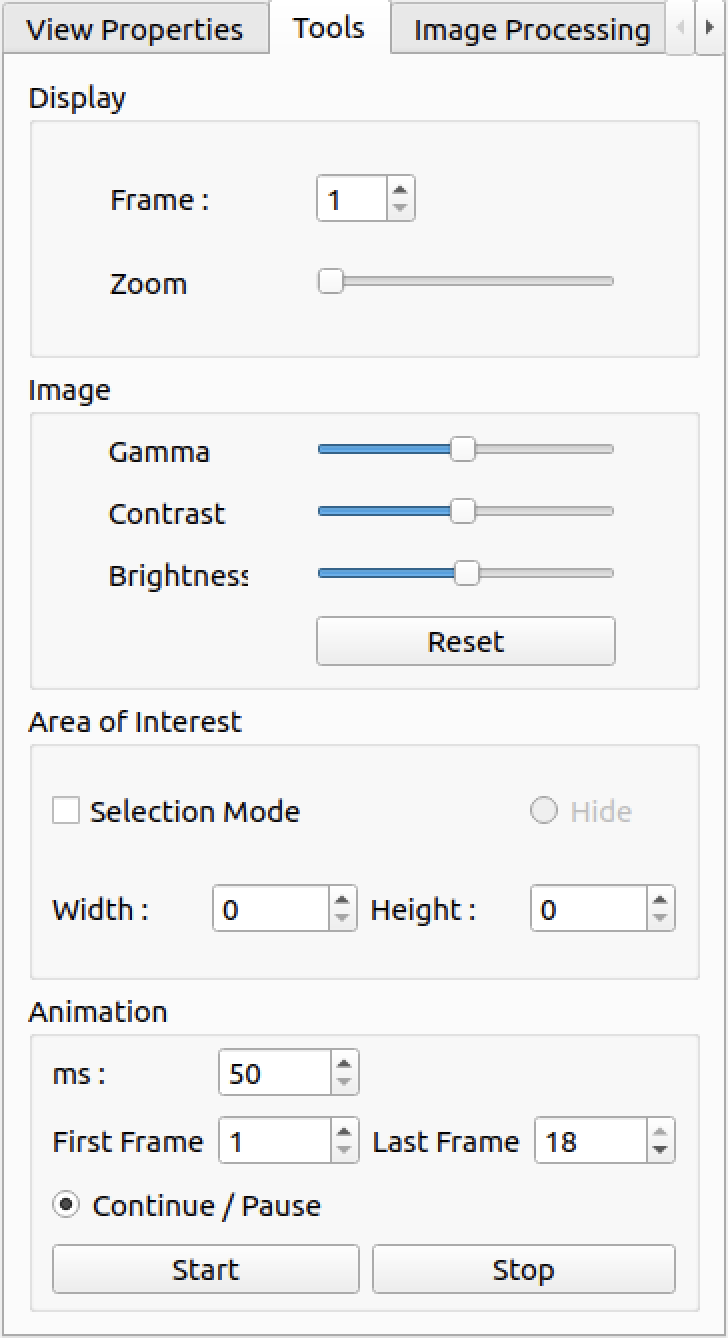
\includegraphics[height=8cm]{media/existing_app/tabs/tools.png}
        \captionsetup{justification=centering}
        \captionof{figure}{Zobrazenie obsahu kariet pravého postranného panelu}
\end {figure}

\clearpage

\subsubsection {Image Processing karta}\label{image_processing_tab}
Na \uv{Image Processing} karte sa nachádzajú tlačidlá ovládajúce manažéra štúdií. Jeho úlohou je zoskupovať rôzne štúdie, v rámci ktorých sa ukladajú parametre jej konfigurácie. Po kliknutí na tlačidlo \uv{Open Study List} sa zobrazí nové okno so všetkými štúdiami a ich parametrami. Pre interakciu s ostatnými poliami na tejto karte je potrebné najprv vytvoriť novú štúdiu kliknutím\newline na tlačidlo \uv{New Study}. Štúdiu je tiež možné ukončiť zvolením tlačidla\newline \uv{Close Study}. Každá štúdia je reprezentovaná jedinečným ID, ktoré sa skladá z dátumu a času jej vytvorenia.

Vytvorením novej štúdie sa aktivujú polia \uv{Image Processing Programs} sekcie. Táto sekcia ponúka tri hlavné zaškrtávacie políčka -- prvé reprezentuje aplikáciu filtra lokálnej variancie. Druhé z nich reprezentuje spustenie algoritmu pre zarovnanie vygenerovanej mriežky s mriežkou myokardu vytvorenou pomocou SPAMM techniky a tretie spustenie algoritmu segmentácie srdečných komôr pomocou grafových rezov. Zaškrtnutím daného políčka a kliknutím na tlačidlo \uv{Run} sa spustí algoritmus príslušný danému políčku. Pre \uv{Grid Tracking} algoritmus je v tejto sekcii možné definovať tri parametre, a to \uv{Curvature Coefficient}, \uv{Force Coefficient} a \uv{Stop Time} (viď \ref{helper_apps}).

\begin {figure}[H]
        \centering
        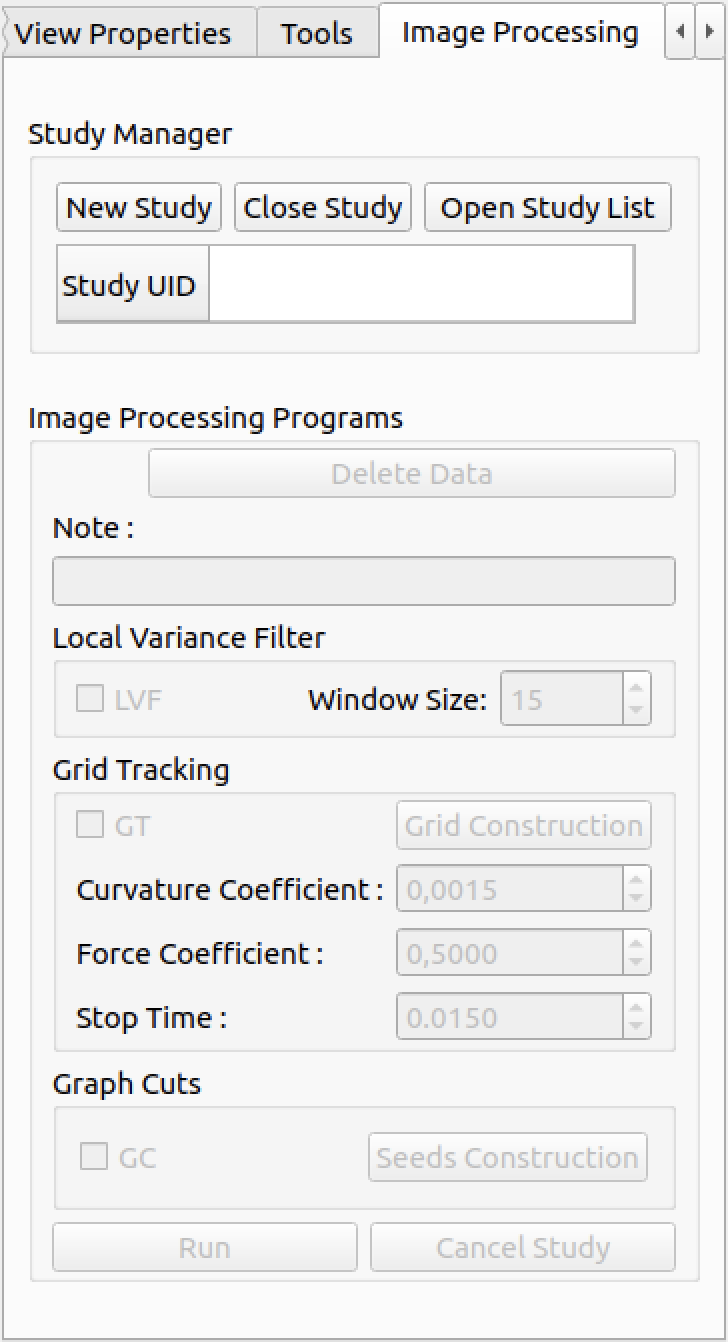
\includegraphics[height=8cm]{media/existing_app/tabs/image_processing_inactive.png}
        \captionsetup{justification=centering}
        \captionof{figure}{Zobrazenie obsahu kariet pravého postranného panelu}
\end {figure}

\subsubsection {History karta}
Účelom poslednej karty \uv{History} je výpis rozličných záznamov pre informovanie používateľa o prebiehajúcich krokov aplikácie.

\begin {figure}[H]
        \centering
        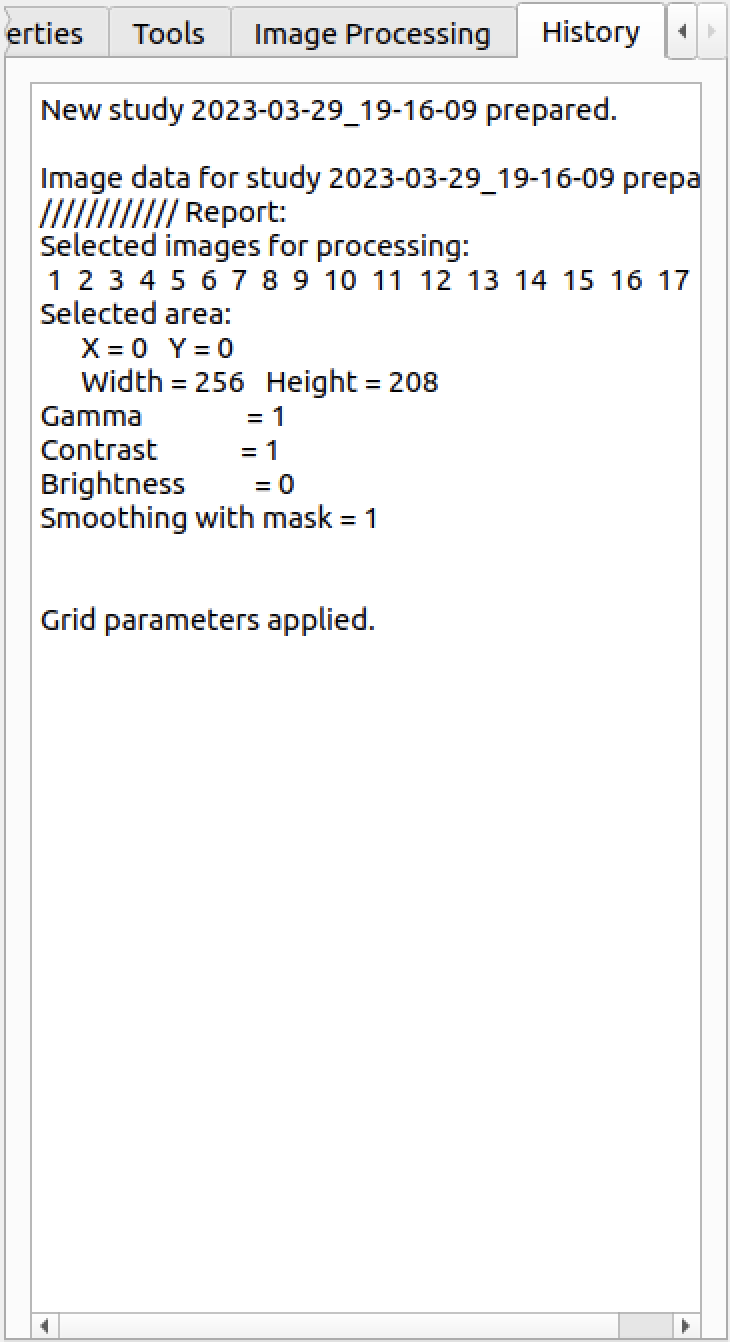
\includegraphics[height=8cm]{media/existing_app/tabs/history.png}
        \captionsetup{justification=centering}
        \captionof{figure}{Zobrazenie obsahu kariet pravého postranného panelu}
\end {figure}

\section {Testovanie a návrhy pre webovú aplikáciu}
Účelom testovania súčasnej aplikácie je zoznámenie sa s aplikáciou a jej procesmi, ako aj overenie jej funkcionality a zistenia používateľského zážitku.

Počas samotného testovania bolo možné úspešne importovať DICOM súbory a zobraziť ich snímky. Snímky bolo taktiež možné animovať na základe nastavenia animácie, zmeniť im kontrast a jas, či ich priblížiť alebo oddialiť.

Následne bola otestovaná funkcionalita týkajúca sa vykreslenia mriežky a jej úprav. Vykreslenie mriežky prebehlo bezchybne -- avšak jej počiatočná poloha bola vždy fixne určená v ľavom hornom okraji snímky.

\clearpage

Toto správanie by sa dalo navrhnúť tak, aby bolo možné určiť počiatočné koordináty vytváranej mriežky jednoduchým kliknutím myši na miesto, kde by mala byť mriežka vykreslená.

Pri priblížení vykreslenej mriežky absentuje posun snímky samotným potiahnutím myši -- posun snímky na ploche bolo možné len pomocou scrollbarov, ktoré boli ťažkopádnejšie na ovládanie.

Taktiež úprava polohy mriežky bola možná len pomocou stlačenia klávesy \texttt{Shift} a potiahnutím myši. Tento spôsob posunu avšak nie je používateľovi nikde odprezentovaný. Návrh používateľského rozhrania webovej aplikácie by mal preto uľahčiť prípadnú zmenu polohy snímky na ploche.

\subsection {Problémy s \texttt{grid-tracker} podprogramom}\label{grid_tracker_issues}
Po úprave polohy mriežky nasledovalo spustenie samotného výpočtu zodpovedného za určenie súradníc bodov mriežok tak, aby zodpovedali vytvorenej mriežke pomocou SPAMM technológie. Pri spustení tohto algoritmu avšak aplikácia spadla. Nasledoval debugging aplikácie, ktorý potvrdil, že daný algoritmus nebol dokončený a prepojený so súčasnou aplikáciou.

Školiteľ bol následne s týmto problémom oboznámený. Po vzájomnej diskusii vzišlo k nasledujúcej dohode -- možnosti prepojenia \texttt{grid-tracker} podprogramu s webovou aplikáciou budú zanalyzované a výsledné prepojenie navrhnuté, avšak následná implementácia prepojenia s týmto podprogramom sa neuskutoční, nakoľko jeho algoritmus bude potrebné upraviť tak aby nielen správne fungoval, ale navyše bol kompatibilný s najnovšou verziou TNL knižnice.

Webová aplikácia bude naďalej prijímať dáta potrebné pre samotný výpočet a odosielať výstup v štruktúrovanej podobe, avšak ten bude do určitej podoby reflektovať prijaté dáta, keďže dané prepojenie s \texttt{grid-tracker} podprogramom nebude implementované. Tento proces prijatia dát, výpočtu a ich odoslanie bude v nasledujúcich častiach spomínaný pod pojmom \uv{SPAMM algoritmus}.
        \chapter {Analýza a návrh webovej aplikácie}
\todo {popísať kapitolu}

\section {Analýza mriežky ako nástroja}
Cieľom tejto sekcie je zhrnúť požiadavky kladené na štruktúru mriežky, ktorá sa bude vykreslovať nad zobrazenými DICOM snímkami. Obsahom tejto sekcie je aj zhrnutie nastaviteľných parametrov tejto mriežky používateľom.

\subsection {Štruktúra mriežky}
Mriežka pozostáva z horizontálnych a vertikálnych úsečok, ktoré sa navzájom pretínajú. Body, v ktorých sa  úsečky pretínajú, nazveme \uv{hlavnými} bodmi. Tie viažu horizontálnu a vertikálnu úsečku prechádzajúcu týmto bodom. To znamená, že posunutím tohto bodu by malo taktiež dojsť k úprave pozícií úsečiek tak, aby stále prechádzali cez presunutý bod.

Okrem spomenutých bodov by mala aplikácia vykresliť aj takzvané \uv{refinement} body na mriežke, ktoré by sa nachádzali medzi bodmi viažucími úsečky. Ich účel je presnejšie zarovnanie mriežky voči mriežke generovanej technikou SPAMM. V súčasnej aplikácii sa generujú tri \uv{refinement} body medzi každými dvoma \uv{hlavnými} bodmi.

Vykreslená mriežka by mala byť interaktívna, t.j. úprava jej celkovej polohy alebo polohy samotného bodu by malo byť možné pomocou pohybom myši.

\subsection {Nastaviteľné parametre mriežky}\label{grid_settings}
Implementácia mriežky by mala obsahovať nastaviteľné parametre, pomocou ktorých by sa dala meniť jej vzhľad, resp. štruktúra.

Zoznam všetkých parametrov mriežky, ktoré by mali byť upraviteľné používateľom, je nasledovný:
\begin {itemize}
\item {uhol mriežky,}
\item {priestor medzi všetkými bodmi,}
\item {X a Y offset mriežky počítaný z ľavého horného rohu snímky a}
\item {počet horizontálnych a vertikálnych úsečiek.}
\end {itemize}

Horeuvedené parametre by mali byť upraviteľné pomocou vstupu na klávesnici.
Taktiež bude môcť byť upraviteľná poloha samotnej mriežky alebo jej akéhokoľvek bodu pomocou myši. Okrem toho by malo byť možné implementovať prepínač, ktorý zaistí zobrazenie \uv{refinement} bodov na vykreslenej mriežke a naopak.

Mriežka by mala na úpravy týchto parametrov reagovať jej prekreslením berúcim do úvahy zmenu daného parametru.

\section {Analýza požiadaviek}
Táto sekcia sa venuje analýze požiadaviek, ktoré sa delia na dve hlavné kategórie -- funkčné a nefunkčné požiadavky. Ich realizácia je nutnosťou pre vytvorenie webovej aplikácie, ktorá bude obsahovať potrebnú funkcionalitu pre základ analýzy srdcového myokardu.

\subsection {Funkčné požiadavky}
Funkčné požiadavky sú požiadavky vymedzujúce rozsah funkcionality, ktorá by mala byť v danej aplikácii implementovaná.

\subsubsection {FR1 -- Spracovanie a zobrazenie MR snímiek}\label{fr1}
Do aplikácie by malo byť možné importovať snímky z magnetickej rezonancie vo formáte DICOM a tieto snímky taktiež zobraziť.

\subsubsection {FR2 -- Animácia MR snímiek}\label{fr2}
Aplikácia by mala umožniť animovať importované snímky pre jednoduchšiu analýzu pohybu myokardu. Parametre animácie ako jej rýchlosť a výber snímky, od/po ktorej/ktorú má animácia prebiehať, by mali byť upraviteľné, napr. pomocou číselného vstupu.

\subsubsection {FR3 -- Zobrazenie a interaktívna úprava mriežky}\label{fr3}
Implementovaná aplikácia by mala vedieť zobraziť mriežku nad snímkou z MR, ktorá by sa mala dať vygenerovať tlačidlom v používateľskom rozhraní.

Mriežka by taktiež mala byť interaktívna, t.j. polohu jej bodov by malo byť možné interaktívne upravovať, napríklad potiahnutím bodu myšou. Parametre mriežky (\ref{grid_settings}) by sa taktiež mali dať upraviť podľa želania používateľa a ich zmena by mala byť ihneď viditeľná.

\subsubsection {FR4 -- Zadanie parametrov pre SPAMM algoritmus}\label{fr4}
Pre korektný výpočet súradníc bodov mriežok je nutné funkčnému SPAMM algoritmu podsunúť rozličné parametre. Ich hodnoty by sa mali dať určiť v aplikácií pre ich neskoršie použitie v tomto algoritme. Výpis týchto parametrov je možné nájsť v \ref{helper_apps}.

\subsubsection {FR5 -- Spustenie SPAMM algoritmu a zobrazenie jeho výsledkov}\label{fr5}
SPAMM algoritmus prijme potrebné dáta o všetkých importovaných snímkach a na nich definovaných mriežkach. Výstupom tohto algoritmu bude štruktúra dát, ktorá bude zodpovedať mriežkam s popisom súradníc bodov. Tento výstup bude následne nutné zobraziť v aplikácii.

\subsection {Nefunkčné požiadavky}
Požiadavky tohto typu síce nevymedzujú rozsah funkcionality danej aplikácie, avšak umožňujú určiť isté obmedzenia pre novú aplikáciu, ako napr. dôraz na podobu výslednej architektúry tejto aplikácie.

\subsubsection {NF1 -- Webová aplikácia}
Prvou nefunkčnou požiadavkou je vytvorenie webovej aplikácie, ktorá by mala byť prístupná zo všetkých moderných webových prehliadačov. Pre lekárov výber tejto architektúry zjednoduší jej prístupnosť, nakoľko k takejto aplikácii bude možné pristupovať z rôznych zariadení a platforiem bez nutnosti inštalácie aplikácie.

\subsubsection {NF2 -- Používateľské rozhranie}
Pre interakciu s aplikáciou je nutné navrhnúť a implementovať používateľské rozhranie, pomocou ktorého bude možné s aplikáciou interagovať. Lekári by preferovali používateľské rozhranie podobné iným aplikáciám z tejto oblasti.

\subsubsection {NF3 -- Ochrana pred únikom dát o pacientovi}
Práca s osobnými dátami by mala byť do maximálnej možnej miere naprieč aplikáciou minimalizovaná, aby sa predišlo únikom citlivých údajov o pacientovi. Týka sa to najmä práce s DICOM súbormi, nakoľko tie obsahujú citlivé dáta o pacientovi.

\section {Používateľské role}
V aplikácii sa bude nachádzať len jeden aktér -- používateľ, rovnako ako v súčasnej aplikácii. Tomuto aktérovi by mala byť aplikácia sprístupnená bez rôznych funkčných obmedzení.

\section {Prípady použitia}
Nasledujúce prípady použitia reprezentujú rôzne činnosti, ktoré môže používateľ s aplikáciou vykonávať. Tieto prípady použitia sú popísané pomocou scenárov, ktoré vychádzajú z funkčných požiadaviek kladených na novú aplikáciu.

Pre lepšiu predstavu sú prípady použitia taktiež znázornené graficky pomocou Use Case diagramu na nasledujúcej strane.

\begin {figure}[H]
        \centering
        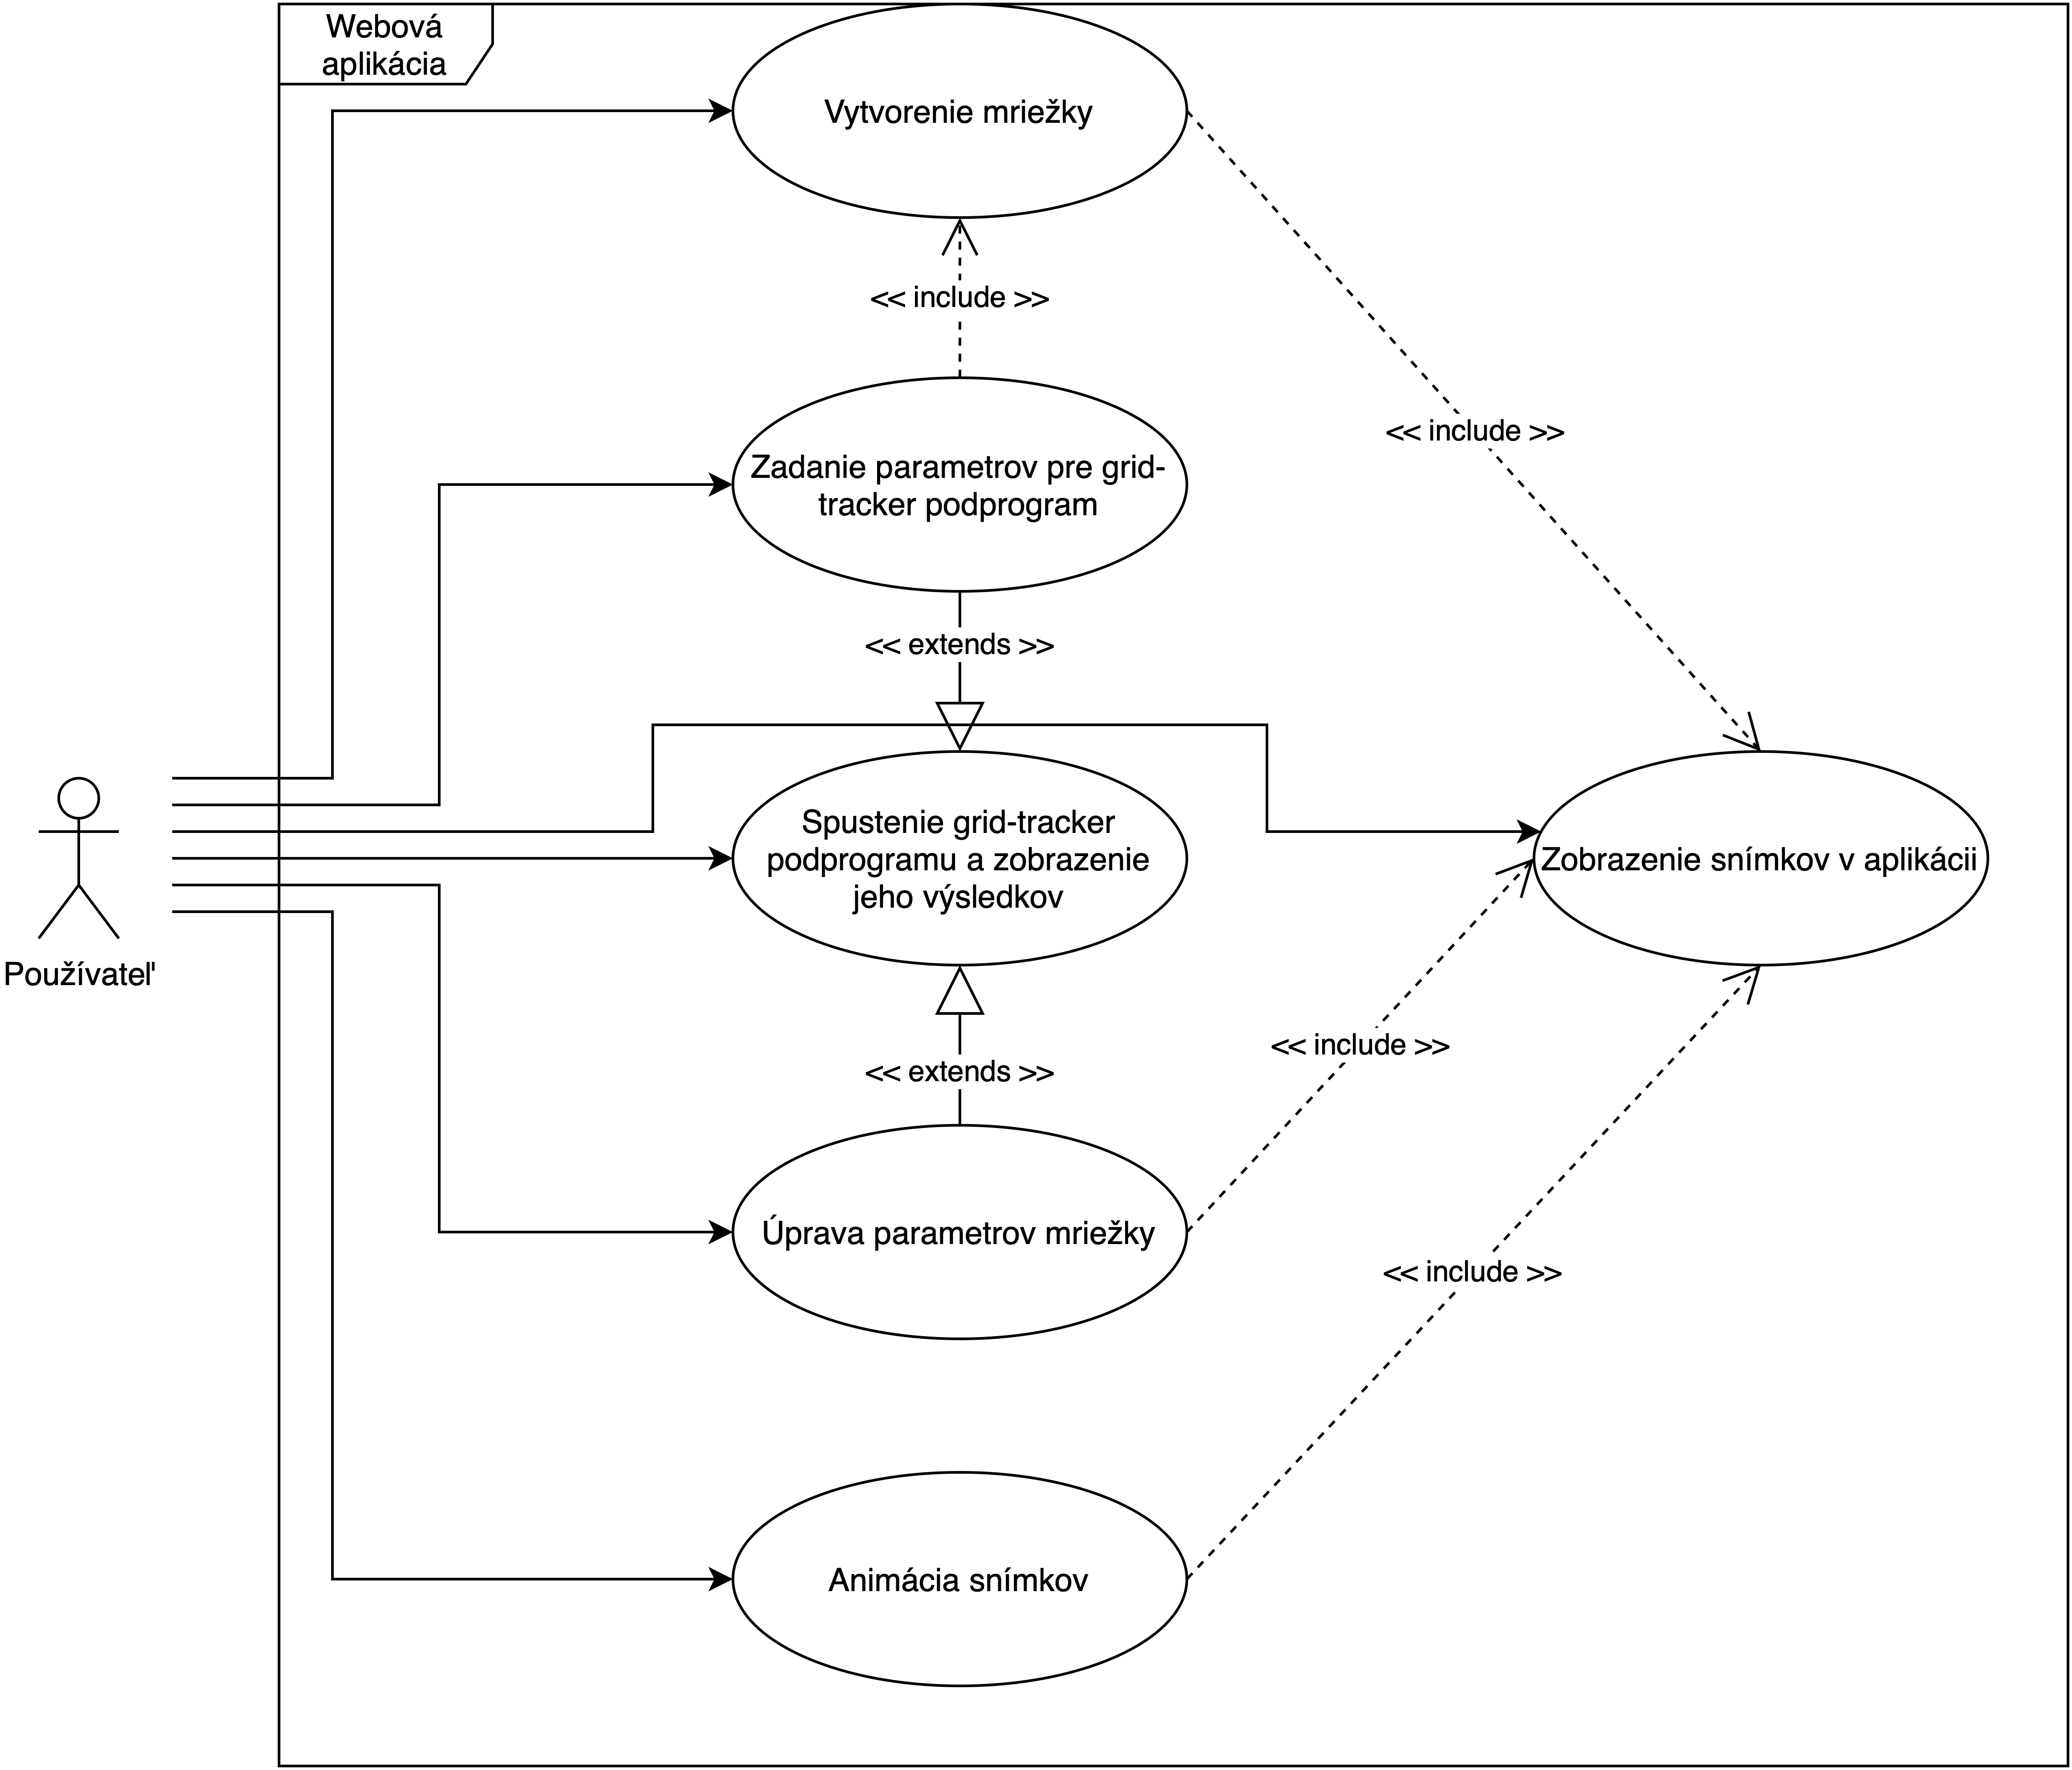
\includegraphics[height=10cm]{media/graphs/usecase.png}
        \captionsetup{justification=centering}
        \captionof{figure}[Use case diagram]{Use case diagram}
\end {figure}

\subsection {UC1 -- Zobrazenie snímiek v aplikácii}\label{uc1}
Zobrazenie snímiek magnetickej rezonancie v DICOM formáte je jedným z esenciálnych funkčných požiadaviek -- \uv{\nameref{fr1}}. Nasledovný scenár túto požiadavku realizuje.

\subsubsection*{Scenár:}
\begin {enumerate}
\item {Používateľ klikne na jedno z tlačidiel pre import DICOM snímiek do aplikácie.}
\item {Prehliadač zobrazí systémové okno, v ktorom si používateľ vyberie snímky, ktoré by chcel mať zobrazené v aplikácii.}
\item {Následne potvrdí import želaných snímiek.}
\item {Aplikácia automaticky vykreslí prvú importovanú snímku a taktiež zobrazí náhľady ostatných importovaných snímiek.}
\item {V prípade, že sa medzi zvolenými snímkami nachádza súbor, ktorý nekorešponduje so štruktúrou DICOM súboru, aplikácia zobrazí notifikáciu o neúspešnom zobrazení snímky.}
\end {enumerate}
	
\subsection {UC2 -- Animácia snímiek}\label{uc2}
Nasledovný scenár realizuje funkciu prehrania série snímiek ako animáciu, ako bolo popísané vo funkčnej požiadavke \uv{\nameref{fr2}}.
Okrem iného taktiež zahŕňa prípad \uv{\nameref{uc1}}. 

\subsubsection*{Scenár:}
\begin {enumerate}
\item {\nameref{uc1}.}
\item {Kliknutím na tlačidlo reprezentujúce štart animácie sa spustí animácia importovaných snímiek.}
\item {Kliknutím na tlačidlo reprezentujúce koniec animácie sa animácia skončí.}
\end {enumerate}

\subsubsection*{Alternatívny scenár:}
\begin {enumerate}
\item [\textbf{2.}] {Používateľ si nastaví rýchlosť animácie, index snímky, od ktorej má animácia začínať alebo index snímky, ktorou má animácia končiť.}
\item  [\textbf{3.}] {Kliknutím na tlačidlo reprezentujúce štart animácie sa spustí animácia importovaných snímiek.}
\item  [\textbf{4.}] {Kliknutím na tlačidlo reprezentujúce koniec animácie sa animácia skončí.}
\end {enumerate}

\subsection {UC3 -- Vytvorenie mriežky}\label{uc3}
Vytvorenie mriežky nad snímkou z MR je potrebné pre účely analýzu pohybu myokardu. Nasledujúci scenár čiastočne realizuje funkčnú požiadavku -- \uv{\nameref{fr3}}. Taktiež zahŕňa prípad použitia \uv{\nameref{uc1}}.

\clearpage

\subsubsection*{Scenár:}
\begin {enumerate}
\item {\nameref{uc1}.}
\item {Používateľ klikne na tlačidlo \uv{Create grid}.}
\item {Aplikácia zobrazí výzvu pre kliknutie na oblasť snímky, kde má byť mriežka vytvorená.}
\item {Používateľ klikne na oblasť snímky, kde chce vytvoriť mriežku.}
\item {Aplikácia vygeneruje mriežku s predvolenými nastaveniami a zobrazí ju na mieste predchádzajúceho kliknutia myši.}
\end {enumerate}

\subsection {UC4 -- Úprava parametrov mriežky}\label{uc4}
Medzi prípady použitia patrí aj úprava parametrov mriežky určenej pre analýzu pohybu srdcového svalu. Nakoľko je najprv potrebné mať mriežku pred jej úpravou vytvorenú, zahŕňa nasledovný scenár aj jej vytvorenie. Ten taktiež čiastočne realizuje funkčnú požiadavku \uv{\nameref{fr3}}.

\subsubsection*{Scenár:}
\begin {enumerate}
\item {\nameref{uc3}.}
\item {Používateľ upraví jeden alebo viacero parametrov uvedených v \ref{grid_settings}.}
\item {Aplikácia následne automaticky vykreslí mriežku na základe upravených parametrov.}
\end {enumerate}

\subsection {UC5 -- Zadanie parametrov pre SPAMM algoritmus}\label{uc5}
Pre spustenie algoritmu zodpovedného pre posun mriežky vytvorenej používateľom voči mriežke vygenerovanej SPAMM technikou je potrebné tomuto algoritmu poslať tri parametre definované v \ref{image_processing_tab}. Tieto parametre budú využité pri použití funkčného SPAMM algoritmu. Nasledujúci scenár tento prípad použitia realizuje spolu s funkčnou požiadavkou -- \uv{\nameref{fr4}}.

\clearpage

\subsubsection*{Scenár:}
\begin {enumerate}
\item {\nameref{uc1}.}
\item {Používateľ zadá číselné hodnoty parametrov \uv{Curvature coefficient}, \newline \uv{Force coefficient} a \uv{Stop time}.}
\end {enumerate}

\subsection {UC6 -- Spustenie SPAMM algoritmu a zobrazenie jeho výsledkov}\label{uc6}
Spustenie algoritmu a zobrazenie jeho výsledku vyžaduje mať importované DICOM snímky spolu s používateľom vytvorenými mriežkami a ich modifikáciami.

To je dôvodom, prečo tento scenár použitia zahŕňa prípady \uv{\nameref{uc1}}, \uv{\nameref{uc3}}, \uv{\nameref{uc4}} a \uv{\nameref{uc5}}. Samotný scenár realizuje funkčnú požiadavku \uv{\nameref{fr5}}.

\subsubsection*{Scenár:}
\begin {enumerate}
\item {\nameref{uc1}}.
\item {\nameref{uc3}}.
\item {\nameref{uc4}}.
\item {\nameref{uc5}}.
\item {Používateľ kliknutím na tlačidlo \uv{Compute} spustí výpočet SPAMM algoritmu.}
\item {Po dokončení výpočtu aplikácia zobrazí mriežky upravené horeuvedeným algoritmom.}
\end {enumerate}

\clearpage

\section {Technológie pre vývoj webovej aplikácie}
V rámci tejto analýzy budú popísané technológie, ktoré budú použité pri vývoji webovej aplikácie. Konkrétne balíčky, príp. závislosti sa v tejto sekcii nachádzať nebudú -- tie budú popísané v kapitole implementácie webovej aplikácie.

\subsection {HTML5}
Pre definovanie štruktúry webového dokumentu a jeho významu bude potrebné použiť značkovací jazyk HTML. Tento jazyk pozostáva zo série značiek (elementov) a k nim príslušných atribútov, pomocou ktorých je možné vytvorený obsah anotovať a významovo ho definovať. Týmto spôsobom je možné vytvoriť nadpisy, odstavce textu, číselné i nečíselné zoznamy, či importovať obrázky alebo sprostredkovať audio/video, atď.

Takto štruktúrovaný dokument definovaný pomocou jazyka HTML je možné zobraziť v ľubovoľnom webovom prehliadači. Webový prehliadač takýto dokument zanalyzuje a na základe použitých značiek vykreslí. Každá značka má definovaný predvolený štýl zobrazenia, ktorý sa môže líšiť od prehliadača k prehliadaču.

Nižšie je uvedený príklad základnej štruktúry HTML5 webového dokumentu:

\begin{minipage}[]{\linewidth}
\begin{minted}{html}
<!doctype html5>
<html>
  <head></head>
  <body>
    <p>Hello world!</p>
  </body>
</html>
\end{minted}
\end{minipage}

Značka \texttt{<!doctype>} definuje verziu použitého HTML dokumentu, čo je v tomto prípade HTML5. Ďalej nasleduje značka \texttt{<html>}, ktorej úloha je zoskupiť elementy \texttt{<head>} a \texttt{<body>}. V elemente \texttt{<head>} sa zvyčajne nachádzajú metadáta ako názov dokumentu, špecifikácia ďalších zdrojov pre načítanie v dokumente a iné. Na druhú stranu, element \texttt{<body>} zoskupuje obsah dokumentu, ktorý je zobrazený prehliadačom.

Prvá verzia tohto jazyka bola definovaná v roku 1993 samotným vynálezcom WWW, Timom Berners-Leeom. Momentálne najnovšou verziou HTML jazyka je tzv. HTML5 Living Standard\footnote{https://html.spec.whatwg.org}, vyvíjaný pracovnou skupinou WHATWG\footnote{https://whatwg.org/} \cite{html_standard} (vlastný preklad).

Najnovší štandard priniesol viacero nových značiek ako napr. \texttt{<audio>} pre prehrávanie audia, \texttt{<video>} pre prehrávanie videa, či \texttt{<picture>}, ktorá je určená pre definovanie viacero zdrojov pre obrázok. HTML5 štandard okrem značiek poskytuje niekoľko API, ktoré sú implementované webovými prehliadačmi. Pomocou nich je možné napr. geolokalizovať používateľa využitím HTML5 Geolocation API alebo vykreslovať grafiku použitím HTML5 Canvas API, a iné.

\subsection {CSS 3}
CSS\footnote{https://developer.mozilla.org/en-US/docs/Web/CSS} -- z anglického Cascading Style Sheets -- je jazyk popisujúci vzhľad použitých HTML5 elementov vo webovom dokumente. Tento jazyk definuje súbor pravidiel, ktoré môžu byť aplikované na jednotlivé elementy webového dokumentu, na základe ktorých sa mení vzhľad pravidlami ovplyvnených elementov.

Samotné pravidlo sa skladá zo selektora, ktorý definuje rozsah elementov, ktoré budú ovplyvnené. Nasleduje zoznam vlastností s ich hodnotami, ktoré majú byť aplikované na samotný selektor. Týmto spôsobom je možné definovať vzhľad nielen jedného, ale aj viacerých elementov vo webovom dokumente pomocou jedného pravidla \cite{css_basics} (vlastný preklad).

Nižšie je uvedený príklad pravidla, ktoré mení farbu textu vo všetkých elementoch \texttt{p} (\texttt{p} definuje odstavec textu) na červenú \cite{css_basics} (vlastný preklad):

\begin{minipage}[]{\linewidth}
\begin{minted}{css}
p {
    color: red;
}
\end{minted}
\end{minipage}

\clearpage

Zoskupené pravidlá sa väčšinou ukladajú do samostatného súboru s príponou \texttt{.css}. Tento súbor je následne nalinkovaný do HTML5 dokumentu pomocou značky \texttt{link}, ktorú prehliadač pri parsovaní dokumentu prečíta a následne aplikuje.

Definovanie samotného selektoru môže byť pre dané pravidlo sofistikovanejšie než ako bolo ukázané v príklade vyššie. Element môže byť špecifikovaný na základe jeho rôznych atribútov, ako ID, zoznam tried, či hodnotou jeho atribútu, atď.

Čo sa týka verzií CSS jazyka, nepoužívajú sa verzie ale tzv. levely. Prvým levelom bol CSS Level 1, ktorý sa stal odporúčanou špecifikáciou W3C konzorcia\footnote{https://www.w3.org} v 1996. Tento level bol základom pre nasledujúce levely tohto jazyka.

V súčasnosti najnovší level CSS jazyka je CSS Level 3, v ktorom sa narozdiel od predchádzajúcich levelov jednotlivé časti jazyka delia na moduly, z ktorých každý môže mať level vyšší než level CSS jazyka. Z tohto dôvodu sa taktiež rozhodlo, že samotný level CSS jazyka sa už nebude zvyšovať \cite{about_css} (vlastný preklad).

\subsection {JavaScript}
JavaScript je cross-platformový skriptovací programovací jazyk a treťou základnou technológiou pre vývoj webových stránok a aplikácií, po HTML a CSS. Používa sa pre implementovanie funkcionality, ktorú nie je možné dosiahnuť pomocou kombinácie HTML a CSS, ako napr. dynamická interakcia používateľa s webovou stránkou/aplikáciou, riešenie rôznych výpočetných úloh, odosielanie dát na server a prijímanie odpovede, a iné.

Samotný jazyk bol vytvorený Brendanom Eichom, pracujúcom vo firme Netscape, ktorá taktiež vyvíjala webový prehliadač -- Netscape Navigator. \newline JavaScript bol zahrnutý už vo verzii 2.0 tohto prehliadača, ktorý bol vydaný v roku 1995. Následne sa začal objavovať aj v iných prehliadačoch -- napr. vo všetkých prehliadačoch vytvorených firmou Microsoft počnúc Internet Explorerom 3.0 \cite{ecmascript_specification} (vlastný preklad). 

JavaScript nasleduje ECMAScript špecifikáciu\footnote{https://tc39.es/ecma262/}, vytvorenú Ecma International organizáciou. Tá kontinuálne vydáva každý rok novú štandardizovanú ECMAScript špecifikáciu, ktorá slúži ako predloha pre vytvorenie všeobecného skriptovacieho jazyka. JavaScript je v tomto prípade jazyk spĺňajúci tento štandard, nakoľko sa ním riadi a implementuje ho. Momentálne najnovšou verziou štandardu je jeho 14. edícia, ktorá pridala najmä nové metódy pracujúce s poľom (\texttt{Array}).

Čo sa týka vlastností samotného jazyka, JavaScript je dynamicky typovaným jazykom, čo znamená, že pri vytváraní premenných sa nedefinuje ich typ. To umožňuje do rovnakej premennej na jednom mieste uložiť číslo, a na inom zase reťazec. Taktiež sa jedná objektovo-orientovaný jazyk, kde dedičnosť je riešená mechanizmom prototypov -- metódy a vlastnosti môžu byť za behu pridané do akéhokoľvek objektu \cite{ecmascript_specification} (vlastný preklad).

JavaScript používa primárne jedno hlavné vlákno pre všetky svoje operácie, avšak je možné vytvoriť tzv. pracovné vlána pomocou Web Workers technológie. Nakoľko JavaScript podporuje OOP, imperatívny a deklaratívny štýl písania kódu, jedná sa o tzv. multi-paradigmový jazyk \cite{ecmascript_specification} (vlastný preklad).

Samotný kód je potrebné uložiť do súboru s koncovkou \texttt{.js}, aby bol rozpoznaný prehliadačom ako súbor obsahujúci JavaScript kód.

\subsubsection {TypeScript}
Pri písaní kódu v JavaScripte sa často môže stať, že programátor napíše nevalidný kód, avšak IDE ho žiadnym spôsobom na túto skutočnosť neupozorní. Táto situácia vzniká najmä kvôli tomu, že sa v JavaScript kóde nevyskytujú žiadne informácie o typoch premenných, argumentov funkcií a iné.

Pri menšom projekte je možné tieto problémy lepšie podchytiť, avšak pri vývoji robustnejšej aplikácie rôznymi ľuďmi je pravdepodobnejšie, že bude obsahovať chyby, na ktoré by mohli byť vývojári upozornení samotným IDE vopred ešte počas vývoja aplikácie.

Problém s neexistujúcimi typmi je možné vyriešiť pomocou písania kódu v jazyku TypeScript, vyvíjanom od jeho počiatku (2012) firmou Microsoft\footnote{https://www.microsoft.com}. Ten pridáva podporu pre typy premenných, vstupných a výstupných argumentov funkcií či návratových hodnôt funkcií.

TS je nadmnožinou JavaScriptu, čo znamená, že validný JavaScript kód je taktiež validným TypeScript kódom. Taktiež je garantované, že JavaScript kód prevedený na TypeScript nezmení správanie kódu, čo znamená pre vývojárov jednoduchšiu migráciu z JavaScriptu do TypeScriptu \cite{about_typescript} (vlastný preklad). TypeScript v princípe funguje ako statický analyzátor kódu, ktorý analyzuje validitu napísaného kódu. V prípade, že kód nie je validný, alebo obsahuje chyby, TypeScript pomocou IDE upozorní vývojára na túto skutočnosť. Pre samotnú analýzu kódu je nutné písať kód do súborov s koncovkou \texttt{.ts}.

Nižšie je uvedený príklad funkcie, ktorej argument má typ \texttt{number}. V prípade, že by bol argument nekompatibilného typu ako v uvedenom príklade, TS compiler pomocou IDE informuje vývojára o tejto skutočnosti. V prípade použitia JavaScriptu by IDE o tomto probléme vývojára neinformovalo. 
\begin{minted}[linenos]{typescript}
function divideByThree(a: number): number {
  return a / 3;
}

divideByThree('a');
// TS compiler v tomto prípade zobrazí na r. 5 nasledujúcu chybu:
// The left-hand side of an arithmetic operation
// must be of type 'any', 'number', 'bigint' or an enum type.
\end{minted}

Nakoľko nie je možné TypeScript použiť priamo vo webovom prehliadači, je potrebné takýto kód konvertovať (transpilovať) do JavaScriptu. Podporu tejto funkcionality pridali vývojári TypeScriptu pomocou konzolového programu \texttt{tsc} \cite{about_typescript} (vlastný preklad). Jeho vstupom sú TypeScript súbory, ktoré majú byť transformované do JavaScriptu. Výstupom sú už súbory v JavaScripte.

Počas transpilácie TypeScript kódu do JavaScriptu dochádza k vymazaniu všetkých informácií o typoch a iných konštruktoch nepodporovaných JavaScriptom, tak aby výsledný kód bol validným JavaScript kódom \cite{about_typescript} (vlastný preklad).

Pre horeuvedené výhody tohto jazyka bude TypeScript použitý pri vývoji webovej aplikácie.

\subsection {Node.js}
Node.js je asynchrónne cross-platform runtime prostredie JavaScriptu, ktoré umožňuje vývojárom exekuovať JavaScript kód mimo prehliadača. Pomocou neho je možné vyvíjať nielen konzolové aplikácie, ale aj budovať škálovateľné webové služby \cite{about_nodejs} (vlastný preklad).

Node.js je open-source projektom a jeho vývoj zastrešuje nadácia OpenJS Foundation \cite{about_nodejs} (vlastný preklad). Podobne ako JavaScript v prehliadači, Node.js používa jedno hlavné vlákno pre exekúciu kódu. Súčasne je nad Node.js vyvíjaných mnoho softvérových riešení (knižníc a frameworkov), ktoré sú dostupné vo forme balíčkov.

Tieto balíčky zvyknú byť dostupné v registri balíčkov pre Node.js -- npm\footnote{https://npmjs.com}. Pomocou rovnomenného terminálového programu je možné (globálne i lokálne) nainštalovať rôzne balíčky, ktoré môžu byť použité pri vývoji aplikácií. Pre inštaláciu balíčka stačí exekuovať príkaz \texttt{npm install [-D] packagename}. Tieto balíčky je taktiež možné spravovať, aktualizovať na novšie verzie či odinštalovať. Počas inštalácie Node.js je automaticky nainštalovaný aj tento balíčkový manažér.

Okrem iného je vďaka Node.js možné používať len jeden programovací jazyk na vývoj oboch častí webových aplikácii -- frontendu a backendu. Tento fakt predstavuje odpadnutie nutnosti ovládať ďalší programovací jazyk pre vývoj webových aplikácií.

Nakoľko je možné vyvíjať webovú aplikáciu v jednom jazyku, čo prináša komfort pre samotného vývojára, bude Node.js použitý na strane backendu pre komunikáciu s frontendom webovej aplikácie.

\subsection {Docker}
Docker je platforma určená pre vývoj a distribúciu aplikácií. Pomocou tejto platformy je možné separovať aplikáciu od infraštruktúry, čo umožňuje zrýchliť distribúciu softvéru \cite{about_docker} (vlastný preklad).

Docker poskytuje možnosť zabaliť aplikáciu a spustiť ju v izolovanom prostredí nazvanom \uv{kontajner}. Tie sú vytvárané tak, aby obsahovali len nástroje potrebné pre beh aplikácie spolu s jej konfiguráciou, čo zrýchluje inicializáciu a spustenie kontajnerov. Kontajnery sú od seba predvolene izolované, avšak je možné dodatočne nastaviť sieťový interface pre komunikáciu medzi nimi \cite{about_docker} (vlastný preklad).

Vytvorenie kontajneru prebieha z objektu nazývanom \uv{Image}. Image je inými slovami šablóna, ktorá definuje, ako má byť vytvorená zabalená aplikácia. Častokrát obsahuje príkazy, ktoré majú za úlohu nainštalovať aplikačné závislosti, nastaviť dodatočné bezpečnostné vlastnosti či otvoriť porty, cez ktoré je možné s danou aplikáciou komunikovať. Tieto príkazy sú následne uložené do súboru zvanom \texttt{Dockerfile}. Z jedného Docker Imagu je možné spustiť viacero kontajnerov, čím sa stáva škálovanie aplikácie ešte jednoduchším.

Novovytvorený image už väčšinou stavia na existujúcom image vytvoreným inou organizáciou, resp. vývojármi. Takéto image je možné nájsť v registri imageov -- v Docker Hube. Pomocou tejto platformy je možné okrem sťahovania rôznych imageov taktiež zdieľať vlastné obrazy s ostatnými.

Keďže použitie Dockeru prináša výhody ohľadom nasadenia aplikácie, bude v tomto prípade využitá táto technológia pre spustenie aplikácie. Použitím Dockeru je taktiež možné vyhnúť sa prípadnou nemožnosťou zostavenia aplikácie, čoho príkladom môže byť problematické zostavenie súčasnej desktopovej aplikácie.

\clearpage

\section {Analýza architektúry webovej aplikácie}
Medzi prvými krokmi pred vývojom webovej aplikácie patrí analýza prípustných možností architektúry navrhovanej aplikácie. V tomto prípade analýza architektúry závisí najmä na prepojení webového rozhrania so súčasnou aplikáciou, a preto je potrebné najprv zanalyzovať dostupné možnosti tohto prepojenia. Po porovnaní dostupných možností je nutné zvoliť jednu z nich. Následne bude možné pokračovať s analýzou technológií, ktoré budú použité pre vývoj aplikácie.

Čo sa týka prepojenia súčasnej aplikácie, resp. výpočetného podprogramu \texttt{grid-tracker} s novou webovou aplikáciou, existujú dve možnosti, ako by mohla daná integrácia prebehnúť. Prvou možnosťou je využitie tzv. C\texttt{++} addons\footnote{https://nodejs.org/docs/latest-v18.x/api/addons.html} technológie, druhou možnosťou sa naskytuje využiť relatívne novú technológiu -- WebAssembly\footnote{https://webassembly.org}.

Nakoľko je potrebné pred samotným prepojením webovej aplikácie s \texttt{grid-tracker} podprogramom samotný podprogram upraviť, táto sekcia poslúži najmä autorom pokračujúcim vo vývoji webovej aplikácie. 

\subsection {C\texttt{++} addons}
C\texttt{++} addons je technológia, ktorá poskytuje rozhranie medzi C/C\texttt{++} knižnicami a JavaScriptom\footnote{https://developer.mozilla.org/en-US/docs/Web/JavaScript} \cite{cpp_addons} (vlastný preklad). Táto technológia je implementovaná v rámci Node.js\footnote{https://nodejs.org/en}, čo je runtime prostredie JavaScriptu, ktoré bude popísané v samostatnej sekcii.

C\texttt{++} addons umožňuje pristupovať k natívnym API operačného systému a taktiež pomáha integrovať C/C\texttt{++} knižnice tretích strán pre ich priame použitie v Node.js. Doporučeným spôsobom písania takýchto addonov je pomocou technológie Node-API\footnote{https://nodejs.org/docs/latest-v18.x/api/n-api.html}, vďaka ktorej je možné vytvoriť Node-API addon v jazyku C \cite{cpp_addons} (vlastný preklad).

Pre písanie Node-API addonov v C\texttt{++} musí byť použitý modul \texttt{node-addon-api}\footnote{https://github.com/nodejs/node-addon-api}, nakoľko ten obsahuje hlavičkové súbory v C\texttt{++} \cite{cpp_addons} (vlastný preklad).

Výhodou použitia Node-API technológie je jej nemennosť v rámci rôznych verzií Node.js, čo zaručuje použitie skompilovaného addonu v rôznych verziách Node.js bez nutnosti jeho prekompilovania pre rozličné verzie Node.js \cite{cpp_addons} (vlastný preklad).

Nástrojom pre zostavenie takéhoto modulu je build systém \texttt{node-gyp}\footnote{https://github.com/nodejs/node-gyp}. Ten používa \texttt{binding.gyp} súbor, ktorý špecifikuje konfiguráciu zostavenia modulu. Táto konfigurácia zahŕňa okrem iného aj cestu k zdrojovým \texttt{.cpp} a \texttt{.h} súborom. Tie musia byť pred zostavením upravené tak, aby používali Node-API rozhranie \cite{cpp_addons} (vlastný preklad).

Tento krok zahŕňa vytvorenie metód, ktoré budú prijímať vstupné a vracať výstupné argumenty pretypované na Node-API typy.

Pred zostavením addonu je potrebné vygenerovať Makefile pre cieľový operačný systém pomocou príkazu \texttt{node-gyp configure}. Pre zostavenie addonu je následne potrebné exekuovať príkaz \texttt{node-gyp build}. Ten skompiluje želané súbory špecifikované v \texttt{binding.gyp} do jediného súboru s príponou \texttt{.node}. Ten je možné importovať ako modul do iného JavaScript modulu pomocou kľúčového slova \texttt{import}\footnote{https://developer.mozilla.org/en-US/docs/Web/JavaScript/Reference/Statements/import}. Po jeho importovaní je možné volať jeho metódy rovnakým spôsobom ako iné JS metódy \cite{cpp_addons} (vlastný preklad).

\subsection {WebAssembly}
WebAssembly je nový typ jazyku, ktorý je možné exekuovať vo všetkých moderných webových prehliadačoch. Jeho hlavnou výsadou je zvýšenie rýchlosti exekuovania kódu oproti JavaScriptu blížiaci sa k skoro natívnej exekúcii kódu naprogramovaného v jazykoch C, C\texttt{++} alebo Rust\footnote{https://www.rust-lang.org} a iné. Je navrhnutý tak, aby mohol fungovať spoločne s JavaScriptom \cite{webassembly_concepts} (vlastný preklad).

\clearpage

Webová platforma sa dá vo všeobecnosti rozdeliť na dve časti:
\begin{itemize}
\item {VM, pomocou ktorej sa exekuuje kód webovej aplikácie a}
\item {webové API, ktoré je poskytnuté vývojárom pre kontrolu rozličných funkcionalít webového prehliadača, resp. zariadenia  \cite{webassembly_concepts} (vlastný preklad).}
\end{itemize}

Historicky VM umožňovala načítať len kód napísaný v JavaScripte. Avšak postupom času sa ukázalo, že JS nie je určený pre aplikácie, ktoré potrebujú väčší výpočetný výkon, ako sú napr. 3D hry, VR/AR, editácia videa či obrázkov a iné.
WebAssembly bolo navrhnutý takým spôsobom, aby tieto problémy vyriešilo, čím by prinieslo prostriedky pre vývoj takýchto aplikácií \cite{webassembly_concepts} (vlastný preklad). 

Pomocou WebAssembly JS API\footnote{https://developer.mozilla.org/en-US/docs/WebAssembly/Using\textunderscore the\textunderscore JavaScript\textunderscore API} je možné načítať WebAssembly moduly -- čo sú moduly v binárnom formáte -- do JavaScript aplikácie a zdieľať s touto aplikáciou funkcionalitu poskytovanú týmito modulmi \cite{webassembly_concepts} (vlastný preklad).

Možností, ako daný modul vytvoriť, je viacero:
\begin {itemize}
\item {portovať C/C\texttt{++} aplikáciu pomocou Emscripten\footnote{https://emscripten.org} technológie,}
\item {písať priamo vo WebAssembly,}
\item {napísať aplikáciu v inom jazyku a kompilovať ju pomocou kompilátora podporujúci WebAssembly výstup, alebo}
\item {použiť AssemblyScript\footnote{https://www.assemblyscript.org}, ktorý je podobný TypeScript\footnote{https://www.typescriptlang.org} jazyku a dá sa priamo skompilovať do WebAssembly \cite{webassembly_concepts} (vlastný preklad).}
\end {itemize}

Nakoľko sa v tomto prípade jedná o C\texttt{++} aplikáciu, bude bližšie analyzovaná prvá možnosť zo všetkých dostupných možností.

\clearpage

Najprv je potrebné stiahnuť a nainštalovať Emscripten kompilátor -- ten umožní skompilovať program v C/C\texttt{++} do modulu vo formáte \texttt{.wasm}, pomocou nástroja \texttt{em++}.

Nástroj \texttt{em++} je možné použiť nasledovným spôosobom:\newline \texttt{em++ sample.cpp -o sample.html} 

Výstupom tohto príkazu sú tri súbory -- \texttt{a.out.js}, \texttt{a.out.wasm} a \texttt{sample.html}. Prvý zo súborov tvorí JS kód, ktorého úloha je prepojiť vygenerovaný WASM modul (druhý súbor) s JS prostredím. Následne je možné tento modul spolu s JS kódom importovať do HTML\footnote{https://developer.mozilla.org/en-US/docs/Web/HTML} stránky, na ktorej sa daný modul exekuuje. Takto importovaný kód v HTML stránke je možné vidieť v súbore \texttt{sample.html} \cite{cpp_to_wasm} (vlastný preklad).

Celý proces je pre ilustráciu zobrazený pomocou diagramu nižšie:
\begin {center}
        \centering
        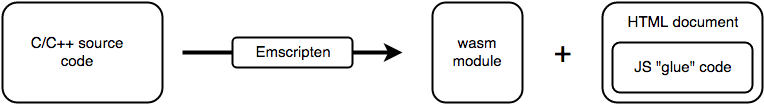
\includegraphics[height=1.75cm]{media/graphs/cpp_to_wasm.png}
        \captionsetup{justification=centering}
        \captionof{figure}{Od zdrojového kódu k .wasm modulu \cite{cpp_to_wasm_image}}
\end {center}

\subsection {Výsledná voľba prepojenia}
C\texttt{++} addons technológia je implementovaná v Node.js, čo by v prípade zvolenia tejto technológie znamenalo zvolenie architektúry klient-server.

Klientom by bol v tomto prípade webový prehliadač, ktorý by posielal HTTP požiadavku serveru s potrebnými dátami pre \texttt{grid-tracker} podprogram. Po skončení výpočtu by server poslal odpoveď s informáciami o bodoch a úsečkách, ktoré by mali byť vykreslené na všetkých importovaných snímkach magnetickej rezonancie.

V prípade použitia technológie WebAssembly by všetky výpočetné operácie mohli byť implementované na úrovni klienta. Tým pádom by nebolo nutné posielať žiadne dáta serveru, čo hrá v prospech bezpečnosti.

Avšak, ako z analýzy \texttt{grid-tracker} podprogramu vyplýva, \texttt{grid-tracker} a TNL knižnica pre zrýchlenie výpočetných algoritmov používajú OpenMP technológiu. Bohužiaľ, WebAssembly túto technológiu nepodporuje, čo by v tomto prípade znamenalo, že by celý výpočet musel prebiehať jednovláknovo alebo byť refaktorovaný tak, aby používal viacero vlákien pomocou technológie WebAssembly threads \cite{webassembly_threads} (vlastný preklad).

Čo sa týka C\texttt{++} addons, tá OpenMP technológiu podporuje. Taktiež by bol v rámci tejto technológie nutný menší zásah do zdrojového kódu \newline \texttt{grid-tracker} podprogramu, nakoľko by stačilo vytvoriť jednu wrapper funkciu v C\texttt{++}, ktorá by bola zodpovedná za konverziu dát do potrebného formátu a jeho výstup.

Taktiež nie je možné spoľahnúť sa na výkon zariadení, na ktorých by bežal \texttt{grid-tracker} pomocou WebAssembly. Nakoľko je tento algoritmus náročný na výpočet, bolo by potrebné zaistiť dostatočné výpočetné prostriedky pre každého lekára využívajúcim webovú aplikáciu.

Na základe týchto dôvodov bude lepšou a istejšou voľbou vybrať si technológiu C\texttt{++} addons, s ktorou by mala byť implementácia prepojenia \texttt{grid-tracker} podprogramu a webovej aplikácie  rýchlejšia a s podporou OpenMP technológie. Výpočty v rámci \texttt{grid-tracker} podprogramu by taktiež neboli závislé na dostupných výpočetných prostriedkov klienta ale serveru, čo umožňuje mať väčšiu kontrolu nad potrebným škálovaním výkonu pre \texttt{grid-tracker} podprogram.

\clearpage

\section {Analýza frameworkov pre tvorbu webovej aplikácie}
Webovú aplikáciu je možné od základov naprogramovať len pomocou vlastného kódu, avšak takýto vývoj by bol nie len zdĺhavejší, ale aj pracnejší, nakoľko by sa musel samotný vývojár zamerať na viac než len na implementáciu samotnej aplikácie. Riešením je použitie webového frameworku, ktorý vývojára od takejto práce odbremenia. 

Pre vývoj webovej aplikácie by bolo vhodné využiť framework, ktorý je postavený nad Node.js technológiou, nakoľko by sa klientská a taktiež serverová časť aplikácie dala naprogramovať v jednom jazyku -- JavaScripte. Plusom by v tomto prípade bolo, ak by daný framework natívne podporoval TypeScript, čo by mohlo zredukovať prípadné množstvo chýb v implementácii webovej aplikácie.
Medzi ďalšími výhodami by patrilo použitie fullstack frameworku, vďaka ktorému by bolo potrebné orientovať sa len v jednom frameworku určenom pre obe časti webovej aplikácie -- frontend aj backend.

V súčasnosti medzi najviac používané fullstackové frameworky, ktoré \newline spĺňajú požiadavky uvedené vyššie, patria Nuxt.js\footnote{https://nuxt.com} a Next.js\footnote{https://nextjs.org}.

\subsection {Nuxt.js}
Nuxt.js je voľne dostupný open-source framework, pomocou ktorého je možné vytvárať fullstack webové aplikácie a stránky pomocou Vue.js\footnote{https://vuejs.org}. Vue.js technológia bude popísaná v samostatnej podsekcii nižšie.

Nuxt.js ponúka automatický routing na základe štruktúry súborov v \newline \texttt{/pages} zložke. Taktiež automaticky delí kód na menšie celky, čo môže pomôcť s prvým načítaním webovej aplikácie. Okrem renderovania obsahu až na klientovi je možné renderovať obsah už na serveri a takýto obsah poslať naspäť webovému prehliadaču. Pomocou automatických importov Vue.js komponentov nie je potrebné explicitne importovať použité Vue.js komponenty \cite{nuxt_introduction} (vlastný preklad).

Samotný framework je naprogramovaný v TypeScripte, čo znamená že je možné využívať type-hinty čo sa týka funkcionality Nuxt.js pri programovaní webovej aplikácie i bez nutnosti použitia TypeScriptu \cite{nuxt_introduction} (vlastný preklad).

Na pozadí používa Nuxt.js Nitro\footnote{https://nitro.unjs.io/} server, ktorý generuje API endpointy na základe štruktúry súborov nachádzajúcich sa v zložke \texttt{server/api} \cite{nuxt_introduction} (vlastný preklad). Nitro je taktiež zodpovedné za zostavenie  aplikácie, pomocou príkazu \texttt{nuxt build} -- jeho výstupom je \texttt{.output} zložka obsahujúca minifikované súbory zbavené všetkých nepoužitých závislostí. Túto zložku je následne možné nasadiť na server podporujúci Node.js a zostavenú aplikáciu spustiť pomocou príkazu \texttt{node .output/server/index.mjs}.

\subsubsection {Vue.js}
Vue.js je JavaScript framework určený pre budovanie používateľského rozhrania postavený na štandardných technológiach ako HTML, CSS a JavaScript.

Tento framework poskytuje deklaratívny programovací model založený na znovupoužiteľných komponentoch, ktoré je možné použiť v rámci iných komponentov, čím pomáha zefektívniť proces vývoja znížením nutnosti použitia duplicitného kódu \cite{vuejs_introduction} (vlastný preklad).

Pod pojmom \uv{komponent} je možné predstaviť si samostatnú jednotku používateľského rozhrania (v HTML) s definovanými štýlmi (pomocou CSS) a stavom, ktorý je riadený pomocou JavaScriptu.

Nasleduje príklad využitia Vue.js frameworku -- pomocou vytvorenia tzv. Single File Componentu (SFC), ktorý v rámci jedného súboru (\texttt{ParagraphComponent.vue}) kombinuje použitie HTML, CSS a JS ako v popise uvádzanom vyššie.

\clearpage
\begin{minipage}[]{\linewidth}
\begin{minted}{html}
// ParagraphComponent.vue
<template>
  <p>{{ paragraphText }}</p>
</template>

<script setup lang='ts'>
import { computed, defineProps } from 'vue';
const props = defineProps({
  text: {
    type: String,
    default: '',
  },
});
const paragraphText = computed(() => {
  return props.text;
});
</script>

<style lang='scss' scoped>
p {
  color: red;
}
</style>
\end{minted}
\end{minipage}

Uvedený príklad demonštruje dve hlavné funkcie Vue.js frameworku:
\begin {itemize}
\item {deklaratívne vykreslovanie a}
\item {reaktivitu \cite{vuejs_introduction} (vlastný preklad).}
\end {itemize}

V prvom prípade sa jedná o rozšírenie štandardného HTML o template syntax -- \{\{ \}\}, ktorý umožňuje dynamicky vykresliť obsah na základe JavaScript stavu.

V uvedenom príklade sa jedná o zobrazenie paragrafu, kde zobrazený text pochádza z premennej \texttt{paragraphText}. Táto premenná obsahuje \texttt{computed} funkciu, ktorá vracia hodnotu \texttt{props.text}.

Táto hodnota pochádza zo šablóny iného komponentu, kde bol tento komponent (\texttt{ParagraphComponent.vue}) importovaný. Nasledujúci príklad ukazuje práve tento prípad.

\clearpage

\begin{minipage}[]{\linewidth}
\begin{minted}{html}
// ArticleComponent.vue

<template>
  <paragraph-component text="Example text">
</template>

<script setup lang='ts'>
import { ParagraphComponent } from './ParagraphComponent.vue';
</script>
\end{minted}
\end{minipage}

V súbore \texttt{ArticleComponent.vue} bol importovaný komponent \newline \texttt{ParagraphComponent.vue}, ktorý definuje atribút \texttt{text} a nastavuje ho na hodnotu \uv{Example text}. Hodnota tejto premennej sa tým pádom spropaguje do
\texttt{ParagraphComponent.vue} komponentu do premennej \texttt{props.text}.

\texttt{props} je objekt, v ktorom je možné nájsť všetky takto definované \texttt{properties}. Ak by sa namiesto fixného textu v atribúte \texttt{text} nachádzala premenná, ktorá by zmenila hodnotu, funkcia \texttt{computed} zaistí, že sa jej vrátená hodnota (\texttt{paragraphText}) zmení na základe detekovanej zmeny jej hodnoty.
Na základe tohto príkladu bola ukázaná sila reaktivity Vue.js frameworku.

Horeuvedeným spôsobom je možné modulárne vytvárať a zobrazovať rozličné komponenty podľa potreby. Taktiež je možné reagovať na rozličné eventy emitované prehliadačom, ako napr. na kliknutie myši na určitý element, posun po webovej stránke, atď.

Nakoľko webový prehliadač neumožňuje priamo importovať Vue.js komponenty, je nutné ich zostavením skonvertovať do JavaScriptu, napr. pomocou nástroja Vite\footnote{https://vitejs.dev} \cite{vuejs_introduction} (vlastný preklad).

Ten je nutné nainštalovať ako závislosť, napr. pomocou nástroja npm. Následne stačí vytvoriť konfiguračný súbor, v ktorom sa definuje zostavovanie Vue.js komponentov a následne pomocou príkazu \texttt{vite build} je možné zostaviť Vue.js komponenty do \texttt{.js} súborov, ktoré môžu byť následne importované do HTML šablóny \cite{vuejs_introduction} (vlastný preklad).

\clearpage

\subsection {Next.js}
Next.js je voľne dostupným, taktiež open-source fullstack frameworkom podobne ako Nuxt.js. Narozdiel od Nuxt.js nepoužíva pre vytváranie znovupoužiteľných UI komponentov knižnicu Vue.js, ale React.js \footnote{https://react.dev/}.

Next.js ponúka nástroje pre vytváranie API endpointov, ktoré musia byť vytvorené v zložke \texttt{pages/api}. Čo sa týka samotnej funkcionality, taktiež podporuje kompilovanie UI komponentov do spustiteľného JS kódu, jeho minifikovanie pre rýchlejší prenos dát medzi serverom a webovým prehliadačom, code-splitting (rozdelenie kódu pre zvýšenie výkonu aplikácie) až po server-side rendering (SSR, vykreslený obsah na serveri sa pošle klientovi). Samotný framework je naprogramovaný pomocou TypeScriptu, takže je možné využívať nápovedu pri programovaní webovej aplikácie pomocou tohto frameworku \cite{nextjs_introduction} (vlastný preklad).

Zostavenie aplikácie je možné príkazom \texttt{next build}. Tento príkaz vytvorí \texttt{.next} zložku obsahujúcu skompilovaný obsah aplikácie. Takto skompilovanú aplikáciu je možné spustiť príkazom \texttt{next start} \cite{nextjs_introduction} (vlastný preklad). 

\subsubsection {React.js}
React.js je JavaScript framework, ktorý poskytuje možnosti pre budovanie používateľského rozhrania. Svojim účelom je podobný Vue.js frameworku a tiež patrí medzi open-source nástroj, ktorý je ale spravovaný firmou Meta\footnote{https://about.meta.com/} \cite{about_react} (vlastný preklad).

React.js sa od Vue.js líši spôsobom definovania komponentu -- nepoužíva SFC pre definovanie štruktúry komponentu, jeho štýlu a stavu. Pre definovanie štruktúry komponentu používa React.js tzv. JSX, ktorý umožňuje písať HTML v JavaScripte \cite{about_react} (vlastný preklad). \clearpage

JSX je oproti HTML striktnejší v tom, že:
\begin{itemize}
\item {samotný komponent musí byť uzatvorený v značke,}
\item {všetky značky musia mať uzatváraciu značku a}
\item {atribúty značiek je potrebné písať v camelCase forme \cite{jsx_rules} (vlastný preklad).}
\end{itemize}

Použitie CSS je v komponente možné pomocou importovania CSS stylesheetu napísaného pre daný komponent \cite{reactjs_stylesheet} (vlastný preklad), alebo importovania tzv. CSS modulu, ktorý je možné prepoužiť viacerými komponentmi \cite{reactjs_stylesheet_module} (vlastný preklad).

Taktiež je možné CSS definovať priamo v JS a ten naviazať priamo na element v komponente. CSS naviazané týmto spôsobom je možné dynamicky meniť v závislosti od vnútorného stavu komponentu.

Takto definovanému komponentu zostáva už len definovať jeho stav. Ten sa definuje pomocou funkcie \texttt{useState}, ktorého argumentom je inicializačná hodnota. Táto funkcia vracia pole, kde na nultom indexe sa nachádza aktuálna hodnota daného stavu a na prvom indexe sa nachádza funkcia, ktorú je možné exekuovať pre aktualizáciu stavu \cite{react_state} (vlastný preklad).

Nasledujúci príklad zobrazuje použitie tejto funkcie:

\begin{minipage}[]{\linewidth}
\begin{minted}{typescript}
import { useState } from 'react';

const [answer, setAnswer] = useState('');
console.log(answer); // výstupom na konzole bude prázdny reťazec
setAnswer('foo');
console.log(answer); // výstupom na konzole bude reťazec 'foo'
\end{minted}
\end{minipage}

\clearpage

Pre predstavu je na nasledujúcom príklade ukázaný rovnaký komponent ako v príklade pre Vue.js, avšak upravený pre React.js framework:

\begin{minipage}[]{\linewidth}
\begin{minted}{typescript}
import 'paragraph.css';

export default function Paragraph({ paragraphText = '' }) {
  return (
    <>
      <p> {paragraphText} </p>
    </>
  );
}
\end{minted}
\end{minipage}

V porovnaní s kódom pre Vue.js je horeuvedený kód kratší, nakoľko neobsahuje \uv{boilerplate} pre definovanie prijímaných properties ako vo Vue.js. Taktiež je automaticky zaistené prepojenie hodnoty \texttt{paragraphText} s vyrenderovaním jeho obsahu v \texttt{<p>} tagu. Pre fungovanie importovania horeuvedeného komponentu je potrebné funkciu, ktorá obsahuje definíciu React.js komponentu, exportovať. Táto povinnosť vo Vue.js odpadá.

Samozrejme je rozsah rozdielov väčší než tie uvedené v tejto práci. Účelom ukážky je informovať o základných rozdieloch vytvárania komponentov v oboch frameworkoch.

\subsection {Výsledná voľba frameworku}
Na základe doterajších skúseností s Vue.js frameworkom by mal byť vývoj aplikácie pomocou Nuxt.js frameworku pre autora plynulejší a menej problematický, keďže autor nemá skúsenosti s React.js a Nuxt.js frameworkom.

\clearpage

\section {Analýza spracovania MR snímiek}
Spracovávanie importovaných MR snímiek by v aplikácii malo prebiehať najmä na strane klienta -- vo webovom prehliadači. Takto zvolený prístup zamedzí prípadnému útočníkovi preniknúť k snímkam a dátam o pacientoch, ktoré by v opačnom prípade museli byť uchovávané na strane servera. Z uvedeného vyplýva, že pre implementáciu aplikácie bude potrebné nájsť JavaScript knižnicu resp. knižnice, ktoré sú schopné spracovať DICOM súbory v prehliadači.

Pod pojmom \uv{spracovať} je myslené: čítanie hlavičky DICOM súborov, zobrazenie snímiek nachádzajúcich sa v týchto súboroch, či možnosť tieto snímky modifikovať. Medzi ďalšie požiadavky kladené na takúto knižnicu patrí jej aktívny vývoj, dostupná dokumentácia a taktiež použiteľnosť knižnice pre produkčné nasadenie. Je možné, že neexistuje daná knižnica spĺňajúca všetky požiadavky, ktoré sú na ňu kladené. V takom prípade by mal byť nájdený mix knižníc, ktoré spolu tieto podmienky spĺňajú.

Bohužiaľ, všetky požiadavky kladené na hľadanú knižnicu nespĺňa ani jedna nájdená knižnica, ale výber viacero knižníc, kde každá z nich implementuje určitú časť požiadaviek a dokopy podmienky kladené na knižnicu vyššie, spĺňajú.

Jedná sa o nasledovné knižnice:
\begin {itemize}
\item {Cornerstone Core,}
\item {Cornerstone DICOM Image Loader a}
\item {Dicom Parser.}
\end {itemize}

\subsection {Cornerstone Core}
Cornerstone Core\footnote{https://github.com/cornerstonejs/cornerstone} je knižnica, ktorá má za úlohu zjednodušiť proces vývoja komplexnejších webových aplikácií, ktoré majú za úlohu zobrazovať snímky akéhokoľvek formátu, vrátane bežných medicínskych snímkových formátov. Taktiež poskytuje API, pomocou ktorého je možné zobrazovať DICOM snímky a meniť ich vlastnosti, ako napr. zvýšiť alebo znížiť jas, priblížiť snímku alebo ju oddialiť, a iné \cite{about_cornerstone_core} (vlastný preklad).

Táto knižnica neimplementuje import DICOM súborov a ich spracovanie. Túto funkcionalitu deleguje na tzv. ImageLoaders. Tie po spracovaní DICOM súborov posunú DICOM dáta cez spoločné rozhranie Cornerstone Core knižnici, ktorá ich nakoniec vykreslí \cite{about_cornerstone_core} (vlastný preklad).

Cieľom tohto prístupu Cornerstone Core knižnice je jej dôraz na minimalizmus a poskytnutie flexibility pri spracovávaní rôznych typov obrazových dát. Použitie Cornerstone Core knižnice pre vývoj špecializovaných aplikácií tohto typu je de-facto štandardom  \cite{about_cornerstone_core} (vlastný preklad).

V súčasnosti sa pripravuje nová \uv{Cornerstone Core} knižnica, ktorej názov sa zmení na \uv{Cornerstone3D}\footnote{https://github.com/cornerstonejs/cornerstone3D-beta}. Keďže je táto knižnica momentálne v beta berzii a stabilná verzia tejto knižnice ešte nebola vydaná, vývoj aplikácie bude postavený na doterajšej Cornerstone Core knižnici.
Momentálne neexistuje alternatíva tejto knižnice, ktorá by sa špecifikovala na túto oblasť.

\subsection {Cornerstone DICOM Image Loader}
Cornerstone DICOM Image Loader\footnote{https://github.com/cornerstonejs/cornerstone3D-beta/tree/main/packages/dicomImageLoader} je tzv. ImageLoader, ktorý je zodpovedný za načítanie a spracovanie DICOM súborov. Použitie tejto knižnice je vynútené Cornerstone Core knižnicou. Táto knižnica podporuje nielen načítanie DICOM súborov cez HTTP protokol, ale aj z lokálneho súborového systému pomocou File API\footnote{https://developer.mozilla.org/en-US/docs/Web/API/File\textunderscore API} implementovaného webovými prehliadačmi \cite{about_cornerstone_dicom_image_loader} (vlastný preklad).

Po načítaní DICOM súborov je ich parsovanie prenechané knižnici Dicom Parser. Nakoľko sa veľkosť týchto súborov môže pohybovať v rádoch megabajtov (MB), samotné parsovanie súborov beží tiež pomocou webovej technológie zvanej Web Workers\footnote{https://developer.mozilla.org/en-US/docs/Web/API/Web\textunderscore Workers\textunderscore API}. Pre začiatok priblížim technológiu Web Workers a následne knižnicu Dicom Parser\footnote{https://github.com/cornerstonejs/dicomParser}.

\subsubsection {Web Workers}
JavaScript je v prehliadači implementovaný ako jednovláknový jazyk využívajúci jedno hlavné vlákno a exekúcia skriptov tohto jazyka prebieha zvyčajne v tomto vlákne. Výpočetne náročné úlohy by avšak mohli vyústiť do zablokovania tohto vlákna, ktoré sa prejavuje nereagovaním prehliadača na rozličné používateľské akcie alebo nevykreslovaním aktualizácií na webovej stránke. Dôvodom zablokovania hlavného vlákna by v tomto prípade bolo využitie všetkých dostupných prostriedkov prioritne pre danú výpočetne náročnú úlohu.

Web Workers technológia je štandardom, ktorý je implementovaný a poskytovaný webovými prehliadačmi umožňujúci exekúciu takýchto úloh, ktoré by inak pri dlhšom spracovávaní mohli dané hlavné vlákno zablokovať.

Pomocou Web Workers je možné predísť zablokovaniu hlavného vlákna jednoduchým vytvorením nového pracovného vlákna pomocou konštruktu \texttt{new Worker(url)}, kde \texttt{url} je adresa skriptu, ktorý má bežať v novom pracovnom vlákne. Takéto pracovné vlákno môže exekuovať JS skript bez zablokovania hlavného vlákna, keďže je od neho nezávislé \cite{using_web_workers} (vlastný preklad).

\subsection {Dicom Parser}
Dicom Parser je knižnica implementujúca parsovanie všetkých známych validných DICOM súborov. Knižnica je navrhnutá pre beh vo všetkých moderných HTML5 prehliadačoch a k svojej funkčnosti nezávisí na iných knižniciach \cite{about_dicom_parser} (vlastný preklad).

Dicom Parser poskytuje globálny objekt \texttt{dicomParser}, ktorý obsahuje viacero metód, z ktorých je najzaujímavejšia metóda \texttt{parseDicom}. Argumentom tejto metódy je \texttt{Uint8Array} pole obsahujúce nespracovaný (raw) obsah DICOM súboru. Výsledkom volania tejto metódy spolu s \texttt{Uint8Array} poľom je \texttt{DataSet} objekt obsahujúci vyparsovaný obsah DICOM súboru.

Alternatívou Dicom Parser knižnice by mohla byť knižnica dcm.js\footnote{https://github.com/dcmjs-org/dcmjs}, avšak vývoj tejto knižnice nie je stále dokončený (nebola zatiaľ vydaná jej stabilná verzia) a sami vývojári varujú pred použitím tejto knižnice v produkčnom prostredí\footnote{https://github.com/dcmjs-org/dcmjs}.

\subsection {Zhrnutie}
Pre zhrnutie informácií v tejto sekcii -- knižnica Cornerstone DICOM Image Loader využíva Web Workers pre vytvorenie nových pracovných vlákien, ktorých úloha je parsovanie DICOM súborov pomocou metódy \texttt{parseDicom} objektu \texttt{dicomParser} pochádzajúceho z Dicom Parser knižnice uvedenej vyššie. Metódou vrátený \texttt{DataSet} objekt je následne poslaný knižnici Cornerstone Core, ktorá sa postará o vykreslenie vyparsovanej DICOM snímky z tohto objektu.

Nasledujúca sekcia sa bude zaoberať analýzou a návrhom, ako vykresliť mriežku na zobrazenú DICOM snímku pomocou knižnice Cornerstone Tools.

\section {Analýza možností implementácie mriežky}
Pre implementáciu mriežky by bolo vhodné použiť knižnicu, pomocou ktorej by bolo možné danú mriežku vykresliť a upravovať podľa potrieb používateľa.

Rodina Cornerstone frameworkov ponúka pre tento účel Cornerstone Tools\footnote{https://github.com/cornerstonejs/cornerstoneTools} framework, ktorý asistuje nielen pri vytváraní rôznych anotácií pre DICOM snímky načítané pomocou Cornerstone Core, ale aj pri ich segmentácii či rôznych meraní. Taktiež ponúka široký počet nástrojov, ktoré môžu dané snímky modifikovať alebo nad týmito snímkami vykreslovať rôzne informácie či lomené čiary.

Prednosťou Cornerstone Tools knižnice je API\footnote{https://tools.cornerstonejs.org/api/}, pomocou ktorého je možné vytvárať nové nástroje, manažovať ich, či importovať/exportovať ich stav.

\subsection {Závislosti knižnice}
Pre využitie tejto knižnice je potrebná nielen Cornerstone Core knižnica, nakoľko je s ňou úzko previazaná, ale aj knižnica Hammer.js\footnote{https://github.com/hammerjs/hammer.js} a Cornerstone Math\footnote{https://github.com/cornerstonejs/cornerstoneMath}.

Cornerstone Tools využíva Cornerstone Core knižnicu pre reagovanie na rôzne eventy, ktoré Conerstone Core knižnica emituje. Na základe týchto eventov môžu nástroje Cornerstone Tools knižnice meniť svoj stav.

Hammer.js knižnica implementuje podporu rozhrania založeného na dotyku namiesto myši. Túto knižnicu je potrebné importovať bez ohľadu na to, či sa plánujú využívať gestá na báze dotyku alebo nie, nakoľko niektoré nástroje sú od tejto knižnice závislé.

Cornerstone Math, ako už názov napovedá, poskytuje rôzne matematické operácie prevažne týkajúce sa vektorovej matematiky. Niektoré nástroje z Cornerstone Tools knižnice ju používajú napr. pre výpočet vzdialenosti medzi rôznymi bodmi.

\subsection {Spôsoby implementácie mriežky}
Nakoľko Cornerstone Tools neobsahuje mriežku ako nástroj, ktorý vie knižnica zobraziť a s ňou ďalej pracovať, bude nutné túto mriežku implementovať od základov.

Táto implementácia môže využívať API poskytované knižnicou, pomocou ktorej by bolo možné danú mriežku implementovať bez zásahu do knižnice alebo bude nutné danú mriežku naprogramovať priamo do knižnice. Obe možnosti implementácie majú svoje výhody a nevýhody.

\subsubsection {Implementácia pomocou Cornerstone Tools API}
Pri implementácii mriežky pomocou dedikovaného API by nebolo potrebné udržiavať vlastnú kópiu Cornerstone Tools knižnice. V tomto prípade by pre využitie rôznych funkcií implementovaných v samotnej knižnici bolo možné vyžadovanú funkcionalitu importovať pomocou metódy \texttt{importInternal(moduleName)}. Nevýhodou tohto spôsobu je nedostatočná flexibilita spojená s nemožnosťou importovania všetkej funkcionality, ktorá by mohla byť pri vývoji potrebná. Ďalším negatívom zvolenia tohto spôsobu by bola nemožnosť upravenia akéhokoľvek kódu v Cornerstone Tools knižnici.

\subsubsection {Implementácia v rámci Cornerstone Tools knižnice}
Na druhú stranu, ak by mala byť mriežka implementovaná priamo v Cornerstone Tools knižnici, odpadol by problém s importovaním teoreticky potrebnej funkcionality, nakoľko by sa dal importovať akýkoľvek modul knižnice priamo pomocou JS konštruktu \texttt{import}, bez nutnosti využitia \texttt{importInternal} metódy.

\subsubsection {Výsledný výber spôsobu implementácie mriežky}
Nakoľko v tomto momente nie je jasné, či bude výsledná implementácia mriežky potrebovať zmenu niektorého zo súborov Cornerstone Tools knižnice, je vhodnejšie začať implementovať mriežku priamo v knižnici. Keď bude implementácia tejto mriežky dokončená, bude nutné posúdiť, či je možné celú funkcionalitu mriežky migrovať do riešenia využívajúceho iba dedikované API pre svoju funkcionalitu.

Ako pri Cornerstone Core, tak aj Cornerstone Tools knižnica bude mať čoskoro svojho nástupcu\footnote{https://github.com/cornerstonejs/cornerstone3D-beta/tree/main/packages/tools}, ktorá bude určená pre Cornerstone3D. Táto nová knižnica je momentálne v aktívnom vývoji a jej stabilná verzia rovnako ako v prípade Cornerstone3D nebola doteraz vydaná. To je dôvodom, prečo bude pri implementácii aplikácie použitá doterajšia verzia Cornerstone Tools knižnice.

\section {Zobrazenie závislostí medzi knižnicami}\label{dependency_graph}
Pre lepšie znázornenie previazania jednotlivých knižníc uvedených v tejto sekcii bol vytvorený diagram tried, na ktorom sú zobrazené instancie tried a závislosti medzi nimi.

\begin {center}
        \centering
        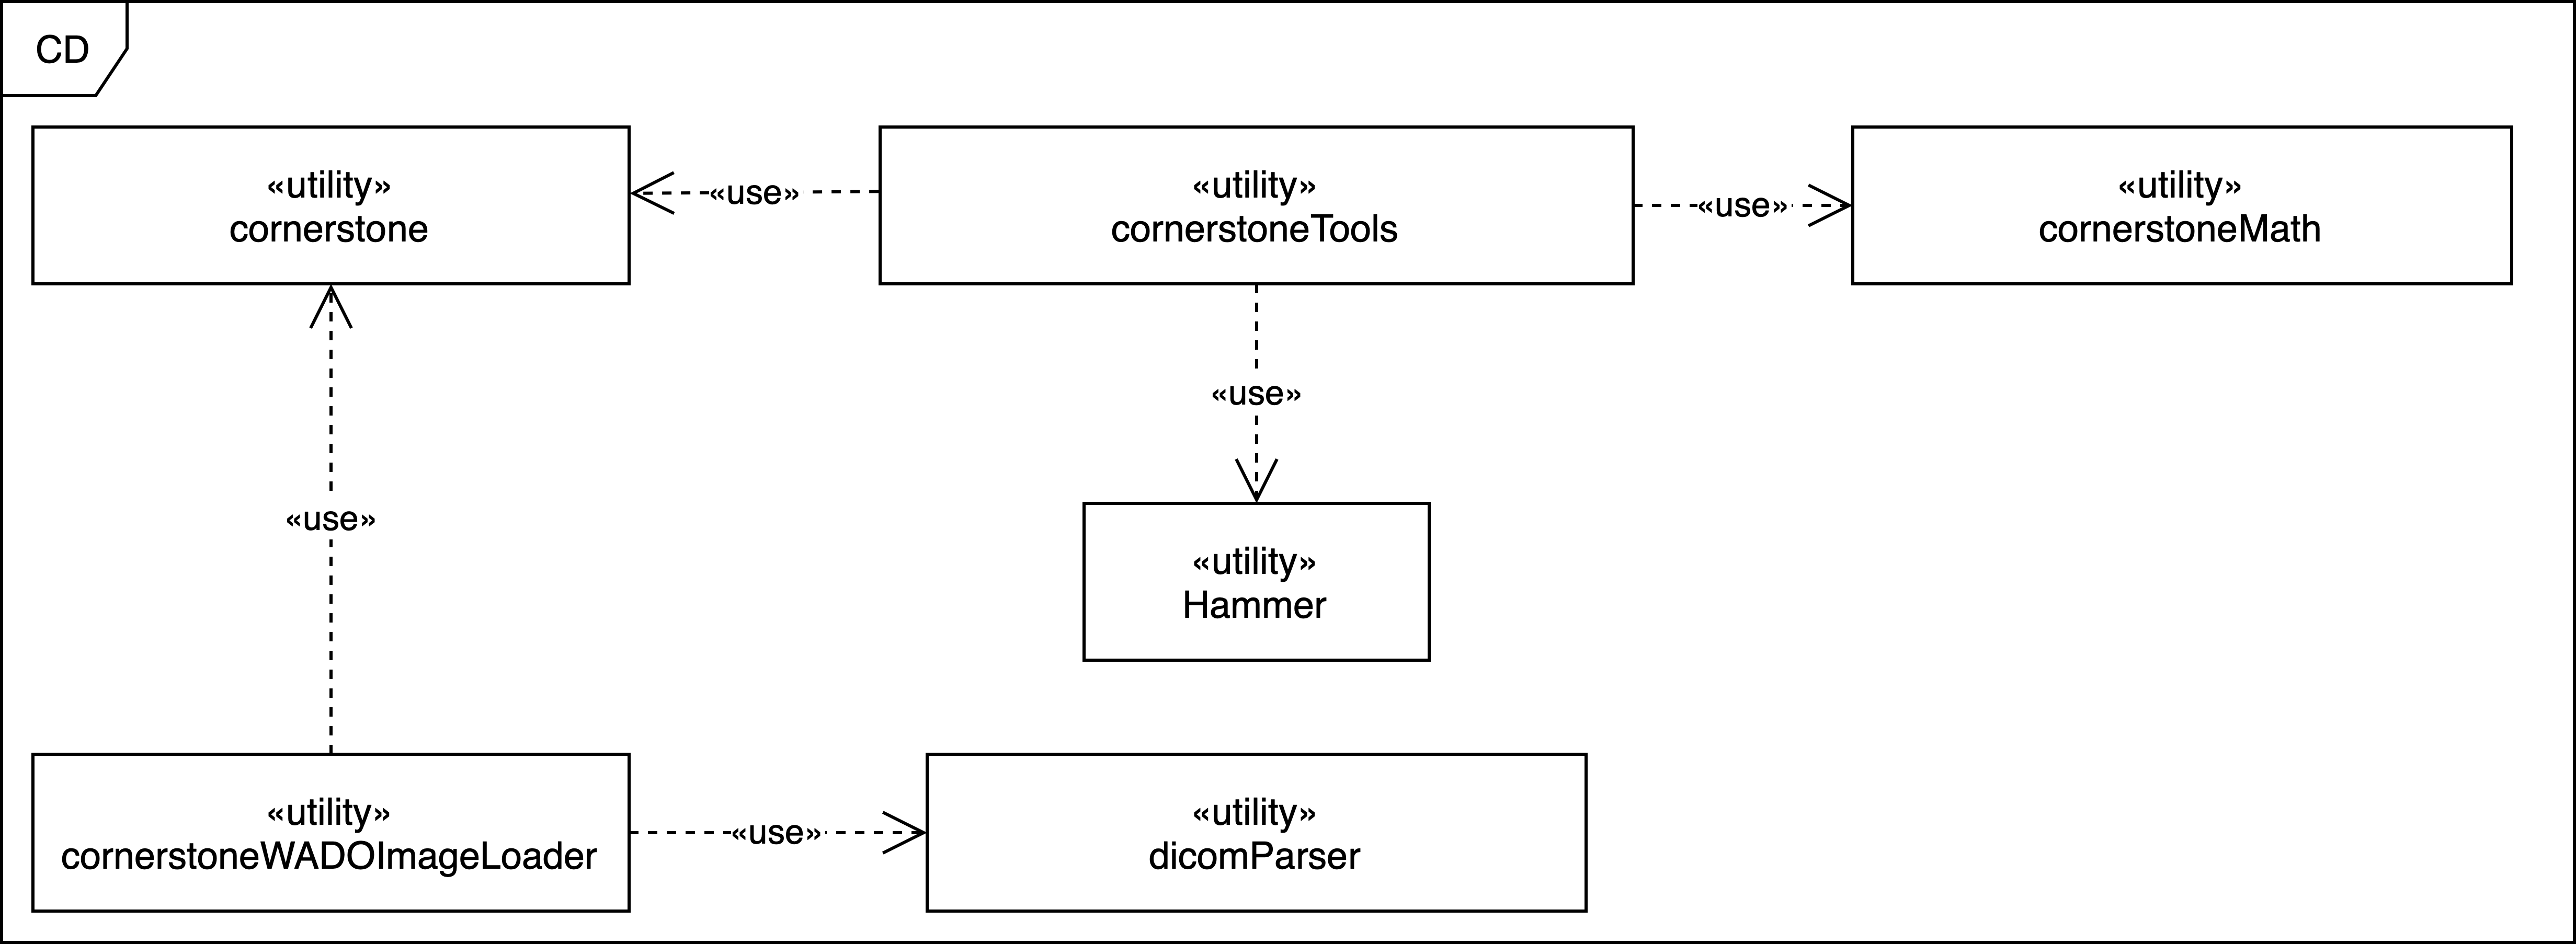
\includegraphics[height=4.75cm]{media/graphs/class_diagram.png}
        \captionsetup{justification=centering}
        \captionof{figure}{Class diagram znázorňujúci závislosti medzi knižnicami}
\end {center}

\clearpage

\section {Návrh používateľského rozhrania}
Pri návrhu používateľského rozhrania som sa inšpiroval UI doterajšej aplikácie, avšak s pár zmenami týkajúcimi sa štruktúry budúceho používateľského rozhrania.

Tento návrh používateľského rozhrania som rozdelil na 4 hlavné časti:
\begin {itemize}
\item {horný panel,}
\item {ľavý postranný panel,}
\item {centrálnu časť a}
\item {pravý postranný panel.}
\end {itemize}

Konečný návrh, ktorý bude slúžiť ako predloha pri vytváraní používateľského rozhrania webovej aplikácie, je priložený nižšie. Ten sa skladá z dvoch snímiek nakoľko sa obsah pravého postranného panelu môže meniť na základe zvolenej karty.

\begin {center}
\centering
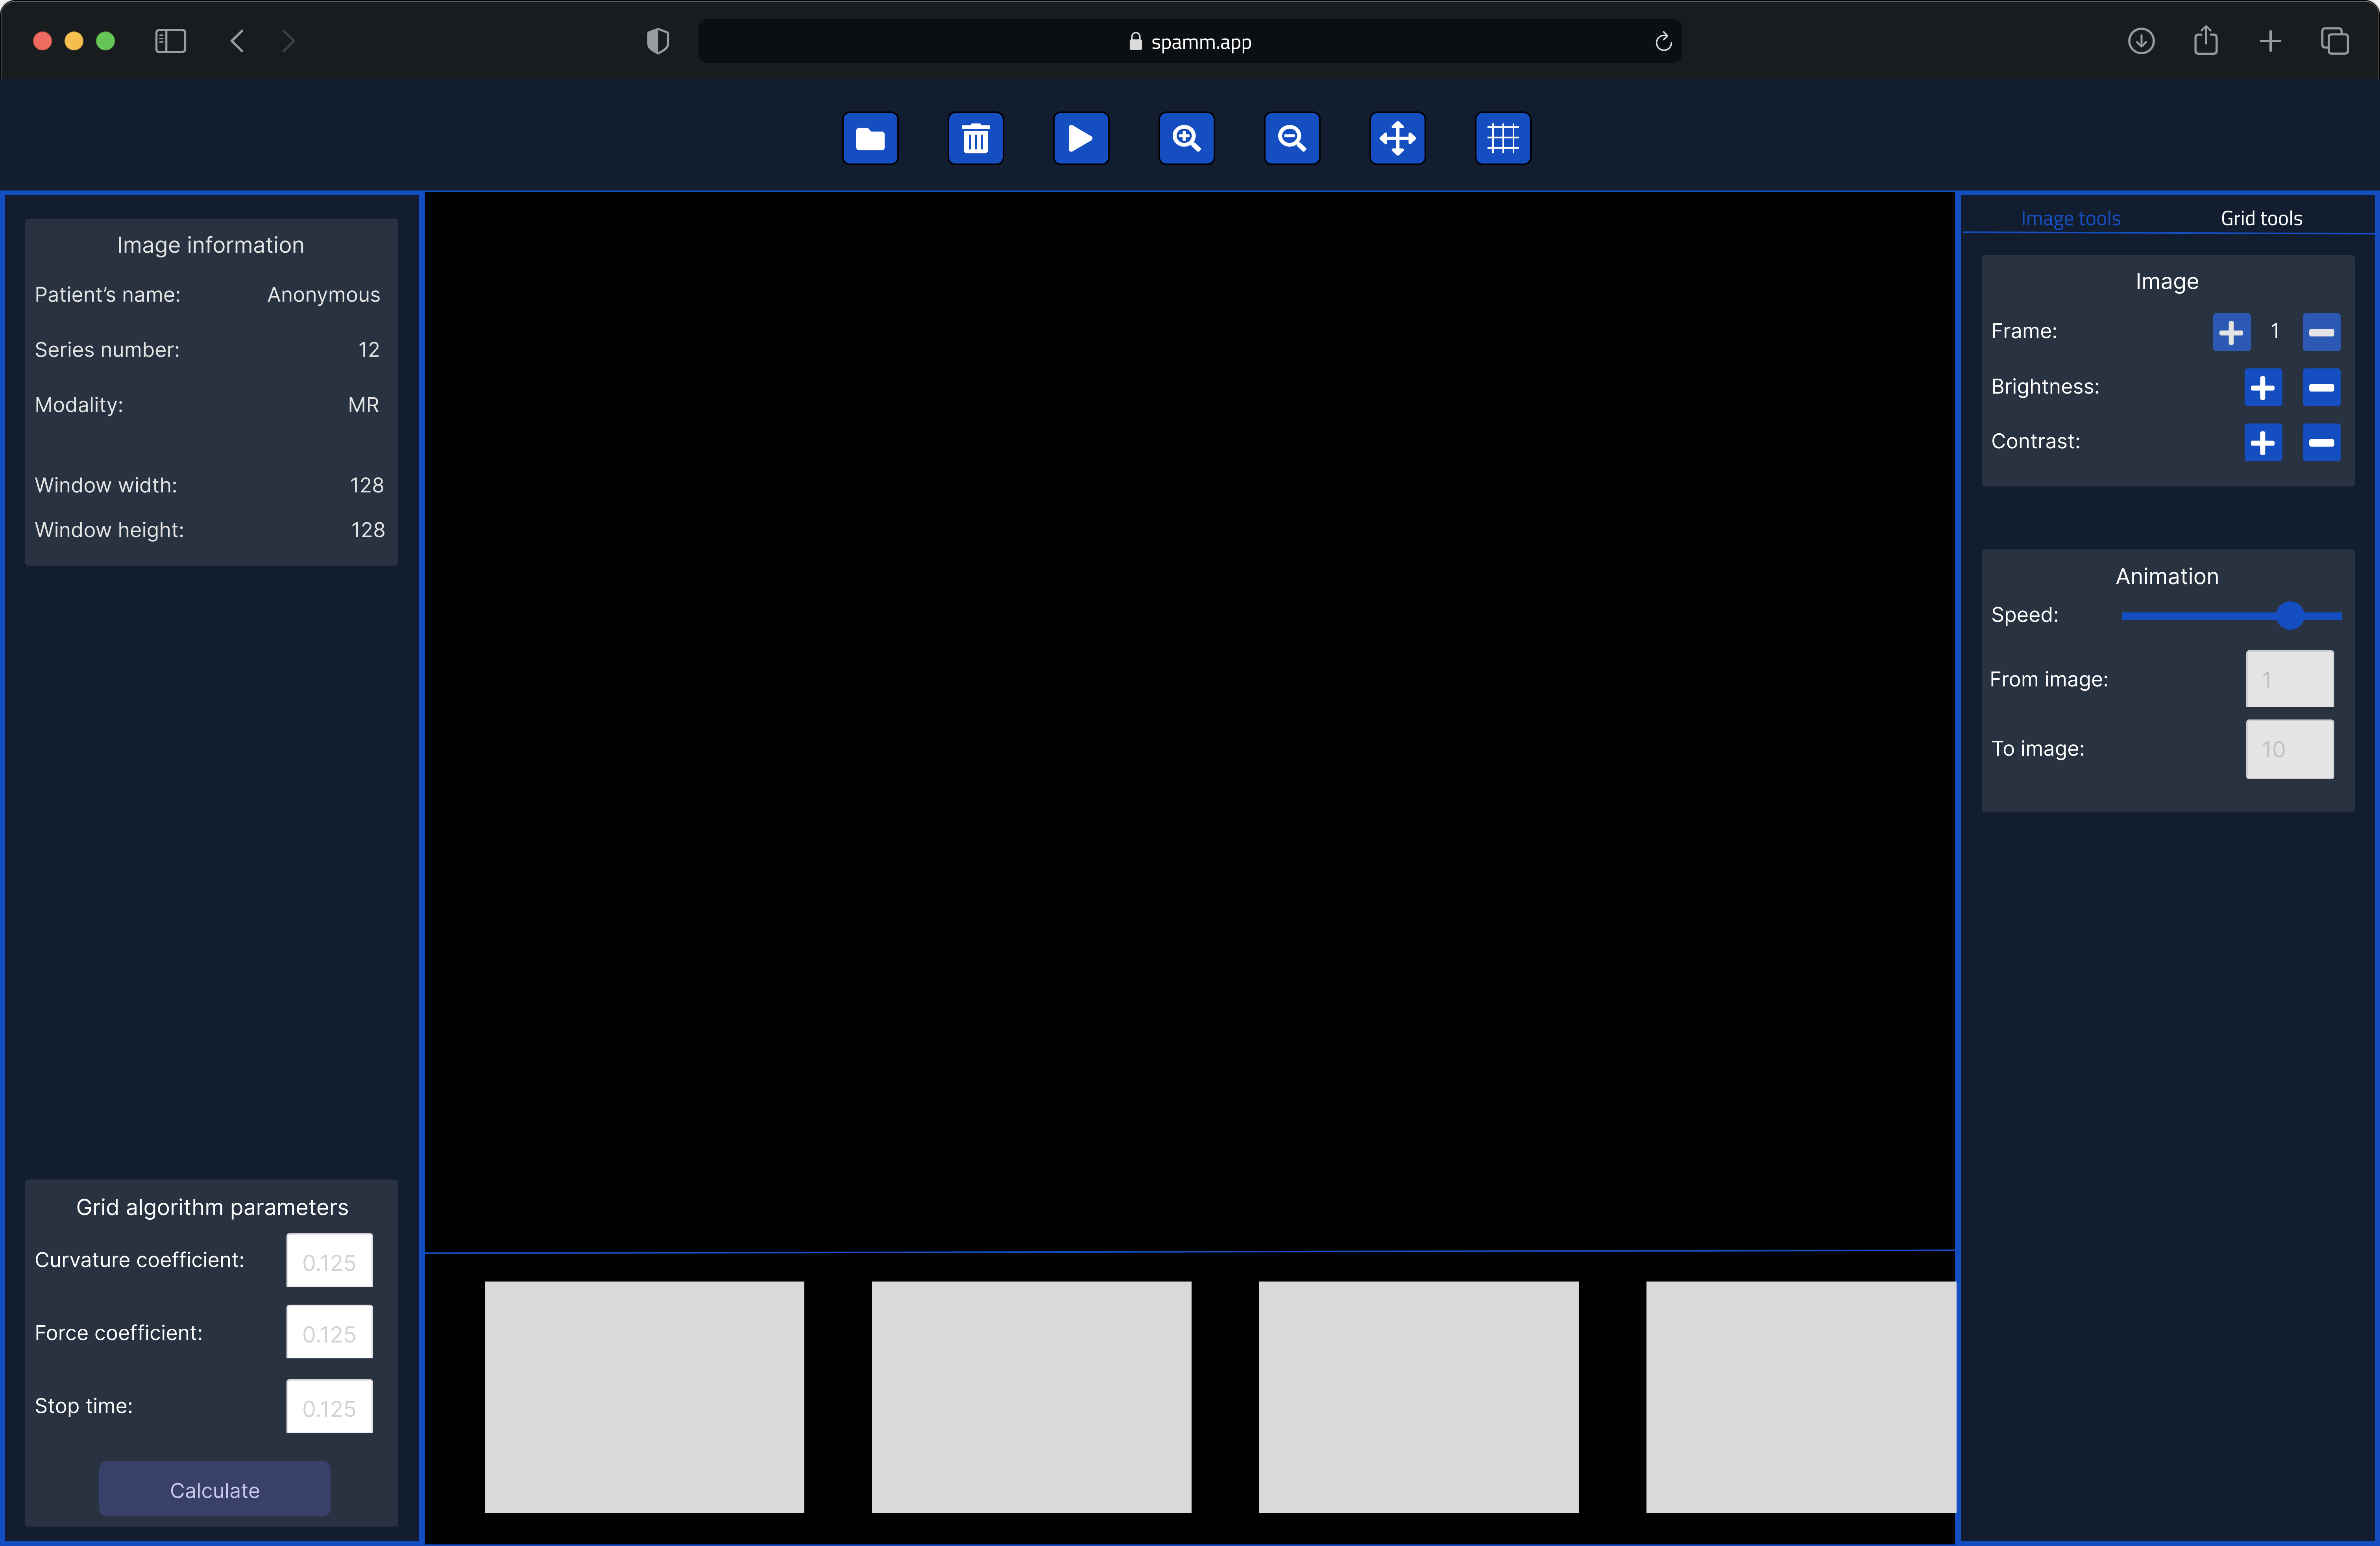
\includegraphics[height=8cm]{media/wireframes/1.png}
\captionsetup{justification=centering}
\captionof{figure}{Návrh používateľského rozhrania - prvá časť}
\end {center}

\begin {center}
\centering
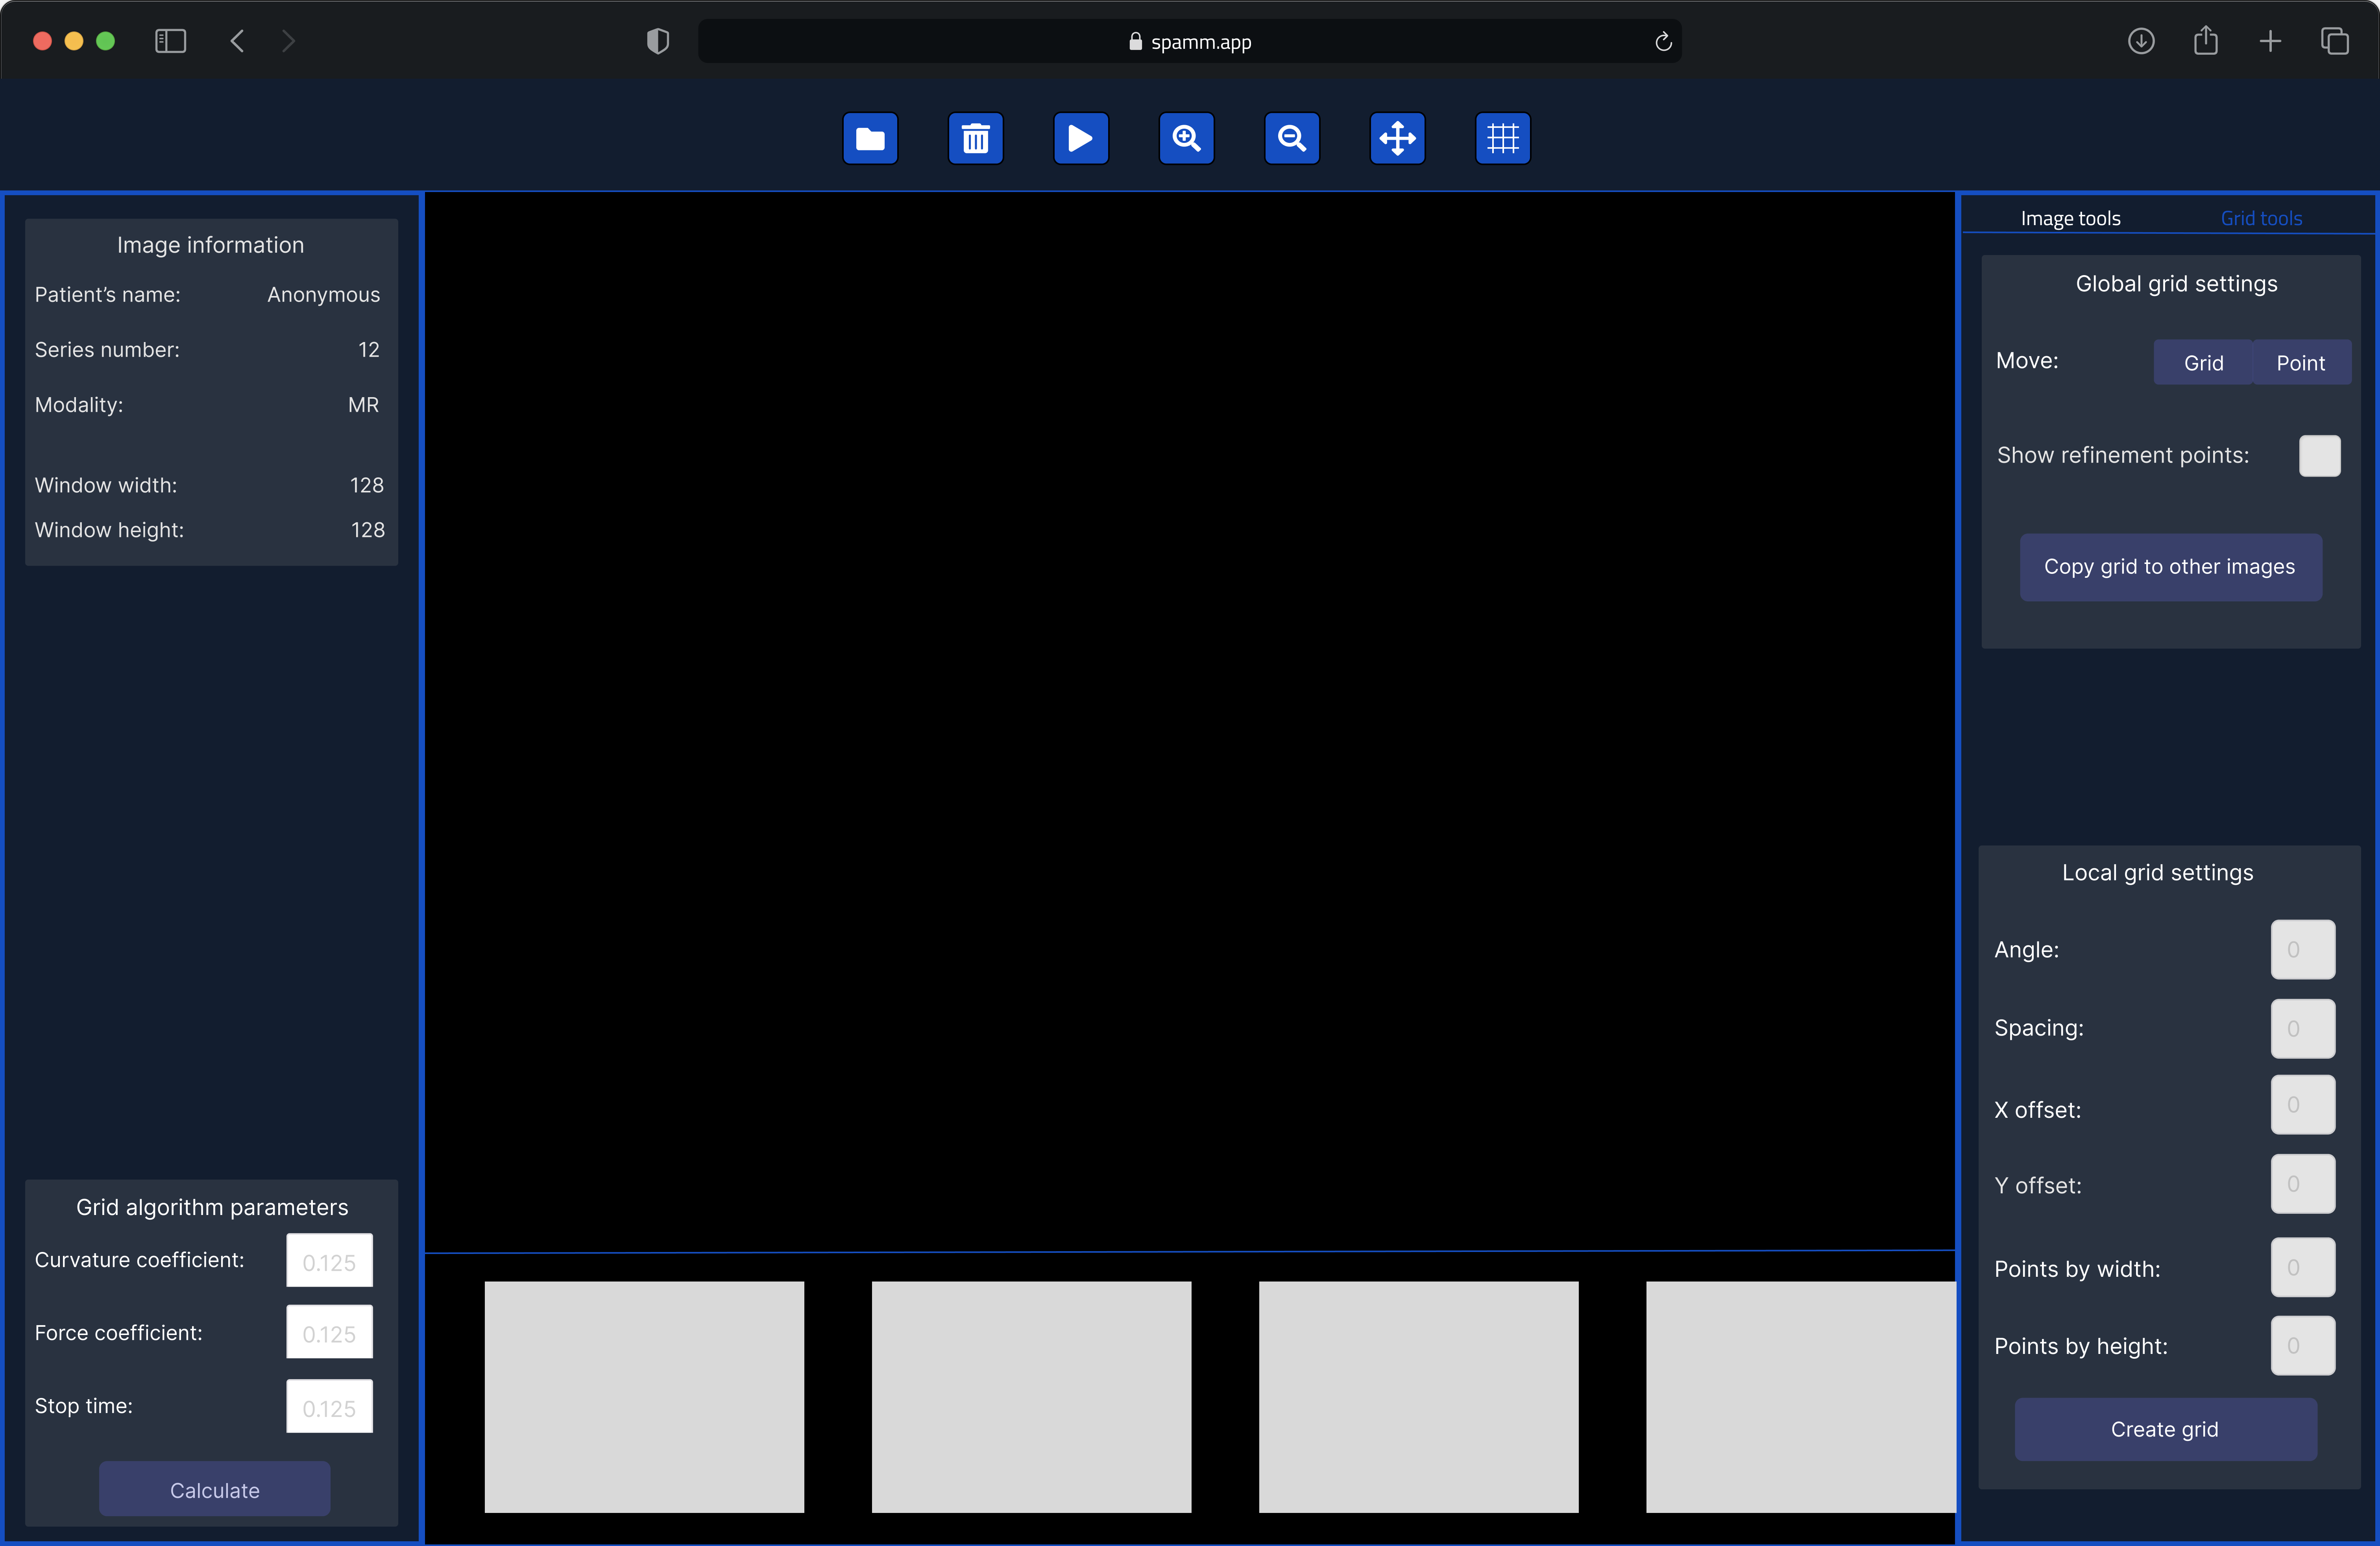
\includegraphics[height=8cm]{media/wireframes/2.png}
\captionsetup{justification=centering}
\captionof{figure}{Návrh používateľského rozhrania - druhá časť}
\end {center}

Nasledujúce podsekcie sa budú venovať popisu jednotlivých častí s popisom jednotlivých možností zobrazených v daných častiach.

\subsection {Horný panel}
V hornom paneli sa nachádzajú tlačidlá, na ktoré bude možné kliknúť.

Prvé tlačidlo zľava slúži pre načítanie DICOM snímiek. Po kliknutí na toto tlačidlo sa zobrazí systémové okno, kde si bude môcť používateľ vybrať DICOM snímky, ktoré sa majú načítať do aplikácie. Pri každej tejto akcii sa vymažú predchádzajúce načítané snímky (ak existujú) a nahradia sa práve zvolenými snímkami.

Akonáhle používateľ aplikácie klikne na druhé tlačidlo, vymažú sa všetky načítané snímky a aplikácia sa prepne do stavu pred načítaním snímiek do aplikácie.

Tretie tlačidlo bude určené pre spustenie animácie snímiek. Po kliknutí naň sa ikona zmení na \uv{stop} ikonu a tlačidlo zmení svoju funkciu -- po opätovnom kliknutí sa animácia zastaví.

Pomocou štvrtého tlačidla bude možné priblížiť aktuálne zobrazenú DICOM snímku -- piate tlačidlo ju oddiali.

Šieste tlačidlo umožní posunúť DICOM snímku v ľubovoľnom smere a siedmym tlačidlom bude možné presúvať vykreslenú mriežku alebo jej body v závislosti na aktuálnom nastavení tohto tlačidla.

\subsection {Centrálna časť}
V centrálnej časti aplikácie bude zobrazená aktuálne vybraná DICOM snímka. Pod touto snímkou budú zobrazené náhľady na všetky importované snímky, na ktoré bude možné kliknúť. Po kliknutí na náhľad snímky sa daná snímka zobrazí. Okrem zobrazenia snímky bude možné vykresliť používateľom definovanú mriežku, s ktorou sa bude dať interagovať pomocou myši.

\subsection {Ľavý postranný panel}
Ľavý postranný panel obsahuje dve sekcie -- \uv{Image information} a \uv{Grid algorithm parameters}.

\uv{Image information} sekcia informuje používateľa o mene pacienta, ktorému aktuálne zobrazená snímka patrí. Okrem mena bude zobrazené číslo série a modalita, ktorej hodnota by pri skenoch MR mala byť rovnomenná. Pod týmito informáciami sa nachádzajú informácie o výške a šírke zobrazenej snímky.

\uv{Grid algorithm parameters} slúži pre nastavenie parametrov pre SPAMM algoritmus. Tieto parametre by mali byť poslané v rámci požiadavky na API endpoint (\ref{api_endpoint}). Tlačidlo \uv{Compute} bude predvolene vypnuté, dokým nebudú vytvorené mriežky na všetkých importovaných DICOM snímkach. V opačnom prípade bude možné kliknúť na toto tlačidlo, ktoré spracuje potrebné informácie z každej snímky a odošle požiadavku na daný API endpoint s ptorebnými informáciami pre aktualizovanie súradníc bodov všetkých mriežok.

\clearpage

\subsection {Pravý postranný panel}
Pravý postranný panel je rozdelený na dve karty -- \uv{Image tools} a \uv{Grid tools}. Pri kliknutí na jednu z možností sa obsah patriaci aktuálne zobrazenej možnosti skryje, aby bolo možné zobraziť obsah zvolenej karty.

\subsubsection {Image tools karta}
Na \uv{Image tools} karte bude možné zvoliť si snímku, ktorá sa má zobraziť. Okrem toho bude možné zmeniť jas a kontrast všetkých snímiek naraz. Pod týmito nastaveniami bude možné upravovať nastavenia animácie snímiek, počínajúc nastavením rýchlosti animácie cez nastavenie počiatočnej a koncovej animovanej snímky.

\subsubsection {Grid tools karta}
\uv{Grid tools} karta bude obsahovať rozličné nastavenia mriežky. Tie sa delia na globálne a lokálne. Globálne nastavenia budú mať efekt pre všetky vytvorené mriežky, lokálne sa budú aplikovať len na mriežku, ktorá je aktuálne zobrazená.

\subsubsection*{Globálne nastavenia mriežky}
V globálnych nastaveniach bude možné nastaviť možnosť interakcie s mriežkou pomocou myši (nastavenie \uv{Move}). Ak bude zapnutá možnosť \uv{Grid}, potiahnutím bodu mriežky sa celá mriežka posunie o vektor posunu. V prípade zvolenej možnosti \uv{Point} sa nebude posúvať celá mriežka, ale iba myšou zvolený bod mriežky.

Ďalšie nastavenie -- \uv{Show refinement points} -- bude slúžiť na dynamické pridanie, resp. odobranie \uv{refinement} bodov zo všetkých mriežok. Tzv. \uv{refinement} body slúžia pre presnejšie zarovnanie používateľom vygenerovanej mriežky so SPAMM mriežkou vygenerovanou MR prístrojom.

Tlačidlo \uv{Copy grid to all images} bude slúžiť pre skopírovanie zobrazenej mriežky do všetkých importovaných mriežok. Po klliknutí na toto tlačidlo sa zobrazí modálne okno, ktoré upozorní používateľa o tejto akcii s nemožnosťou prípadného vrátenia tohto kroku. Toto tlačidlo bude aktívne iba v prípade, že na aktuálnej snímke bude zobrazená mriežka.

\subsubsection* {Lokálne nastavenia mriežky}
V lokálnych nastaveniach bude možné nastaviť rôzne parametre zobrazenej mriežky ako uhol, offset a iné. Pomocou tlačidla \uv{Create grid} bude možné vytvoriť mriežku s predvolenými nastaveniami. Po kliknutí naň sa tlačidlo zmení na \uv{Remove grid}, ktorého funkcia bude spočívať vo vymazaní mriežky na zobrazenej snímke.

\section {Návrh komunikácie webového rozhrania so serverom}\label{api_endpoint}
Pre potrebu komunikácie medzi serverom a klientom bude túto komunikáciu potrebnú navrhnúť. 

Serveru bude nutné posielať potrebné dáta o používateľom definovaných mriežkach pre výpočet aktualizovaných súradníc bodov mriežok. Odpoveď klientovi by mala obsahovať aktualizované súradnice mriežok, ktoré webová aplikácia následne vykreslí.

V tomto prípade stačí, ak server bude poskytovať jeden REST API endpoint, ktorý potrebné dáta príjme, spracuje a odpoveď pošle klientovi vo dohodnutom formáte.

Detaily o tomto API endpointe sú nasledovné:
\begin {itemize}
\item {pre komunikáciu s endpointom bude využitý HTTP protokol,}
\item {endpoint bude dostupný na adrese \texttt{<hostname>/api/grid},}
\item {endpoint prijme dáta vtedy, ak daná požiadavka bude poslaná metódou POST,}
\item {telo požiadavky a odpovede budú vo formáte JSON.}
\end {itemize}

\clearpage

\subsection {HTTP požiadavka}

Telo požiadavky bude mať nasledovný formát, ktorý je avšak pre popis typov premenných popísaný v TypeScripte:

\begin{minipage}[]{\linewidth}
\begin{minted}{typescript}
{
  "data": [{
      "image": {
        "imageId": string;
        "imageData": Uint8Array;
      },
      "grid": {
        "includesRefinementPoints": boolean;
        "primaryLines": [{
            "points": [{
                "x": number;
                "y": number;
                "isCommonPoint": boolean;
              },
              ...
            ]
          },
          ...
        ]
      }
    }
  ]
}
\end{minted}
\end{minipage}

V \texttt{data} poli sa budú nachádzať objekty, z ktorých každý objekt bude reprezentovať jednu entitu skladajúcu sa zo štruktúry snímky (kľúč \texttt{image}) a jej mriežky (kľúč \texttt{grid}).

Kľúč \texttt{image} je objektom, ktorý obsahuje \texttt{imageId} a \texttt{imageData}. \texttt{imageId} je reťazec reprezentujúci ID snímky a \texttt{imageData} pole reprezentujúce raw dáta DICOM súboru.

Kľúč \texttt{grid} je taktiež objektom obsahujúci dva kľúče -- \texttt{primaryLines} a \newline \texttt{includesRefinementPoints}.

\texttt{primaryLines} reprezentuje pole zvislých úsečiek idúcich zľava doprava.
Každá táto úsečka obsahuje pole \texttt{points}.

Toto pole obsahuje objekty reprezentujúce body na danej úsečke. Každý bod sa skladá z troch kľúčov objektu -- \texttt{x}, \texttt{y} a \texttt{isCommonPoint}. \texttt{x} reprezentuje x-súradnicu bodu, \texttt{y} invertovanú y-súradnicu a \texttt{isCommonPoint} značí, či je daný bod \uv{common point} (tzv. bod, v ktorom sa pretína vodorovná a zvislá úsečka mriežky) alebo \uv{refinement point}, pomocou ktorého je možné upresniť polohu mriežky. 

\texttt{includesRefinementPoints} značí, či sa v poli \texttt{points} nachádzajú aj tzv. \uv{refinement} body .

Používateľ iniciuje poslanie dát v tejto štruktúre kliknutím na tlačidlo \uv{Compute}.

\subsubsection {Anonymizácia DICOM dát}
Nakoľko pre účely následného spracovania mriežok na serveri budú taktiež potrebné poslať snímky v DICOM formáte (kľúč \texttt{imageData}), bude nevyhnutné ich pred ich odoslaním na server anonymizovať takým spôsobom, aby nebolo možné spojiť snímky z magnetickej rezonancie s konkrétnym pacientom. Podľa \cite{Varma_2012} (vlastný preklad) je nutné anonymizovať všetky DICOM tagy nachádzajúce sa v skupinách \uv{0008} a \uv{0010}. Skupina \uv{0008} obsahuje dáta ohľadom štúdie a skupina \uv{0010} obsahuje dáta o pacientovi.

Pre tento účel bude potrebné vytvoriť triedu reprezentujúcu DICOM anonymizér, ktorý bude implementovaný v JavaScripte. Táto trieda nahradí obsah tagov z horeuvedených skupín prázdnym reťazcom s dĺžkou daného tagu, aby nenastala inkonzistencia v DICOM dátach. Takto upravené dáta bude môcť byť následné bezpečne poslané na server.

\todo{pridať diagram fyzickej štruktúry, skontrolovať citácie}

\clearpage

\subsection{HTTP odpoveď}

Telo odpovede servera na požiadavku, ktorá bude obsahovať dáta o odoslaných mriežkach, bude v nasledujúcom formáte:

\begin{minipage}[]{\linewidth}
\begin{minted}{typescript}
{
  "grids": [{
    "imageId": string;
    "primaryLines": [{
      "points": [{
        "x": number;
        "y": number;
        "isCommonPoint": boolean;
      },
      ...
      ]
    },
    ...
    ]
  },
  ...
  ]
}
\end{minted}
\end{minipage}

Odpoveď obsahuje kľúč \texttt{grids}, ktorý obsahuje objekty mriežok. Každý z týchto objektov obsahuje kľúč \texttt{imageId} a \texttt{primaryLines}.

Pomocou kľúča \texttt{imageId} je možné spárovať objekt mriežky v odpovedi s mriežkou v aplikácii. Obsahom kľúča \texttt{primaryLines} je pole zvislých úsečiek mriežky idúce zľava doprava.

Každá takáto úsečka obsahuje kľúč \texttt{points} reprezentujúce pole bodov zhora nadol. Každý bod obsahuje svoje súradnice (\texttt{x} a \texttt{y}) a značku, či je bodom, v ktorom sa pretína vodorovná a zvislá úsečka mriežky alebo nie.
        \chapter {Implementácia}

\section {Frontend}

\subsection {Používateľské rozhranie}

\subsection {Spracovanie DICOM dát}

\subsection {Interaktívna úprava mriežky}

\section {Backend}

\subsection {Výpočet umiestnenia mriežky}
        \chapter {Testovanie}
Testovanie je neoddeliteľnou súčasťou vývojového procesu aplikácie. To isté platí pre vyvinutú webovú aplikáciu v rámci tejto diplomovej práce.

Po dokončení jej implementácie bola aplikácia zverená trom testerom -- Erikovi Ekeovi, Timei Bartalskej a ZZZ. ZZZ je odborníkom na magnetickú rezonanciu, ktorého momentálne pracovisko je Institut klinické a experimentální medicíny (IKEM) v Prahe. \todo {doplniť meno testera z IKEMU sem a do poďakovania}

\section {Zoznam zaznamenaných problémov aplikácie}
Testovanie aplikácie prebehlo podľa scenárov všetkých prípadov použitia. Výsledkom testovania webovej aplikáce boli nasledujúce pripomienky:
\begin {itemize}
\item {nefunguje nastavenie rýchlosti animácie počas animácie snímok,}
\item {zoomovanie alebo odzoomovanie snímky nie je možné v niektorých prípadoch zastaviť,}
\item {neočakávané správanie polí pre zadávanie $x$ a $y$ offsetov mriežky,}
\item {nemožnosť opustiť aktivovaný nástroj pre pohyb snímky,}
\item {nemožnosť scrollovania pre zmenu indexu zobrazenej snímky a}
\item {absencia automatického zapnutia nástroja pre pohyb s mriežkou pri zmene jej módu}
\end {itemize}

Tieto pripomienky boli do webovej aplikácie riadne zapracované a verifikované samotnými testermi.
Príčiny týchto problémov je možné nájsť v nasledujúcej sekcii.

\section {Popis príčin zaznamenaných problémov}
Nefunkčné nastavenie rýchlosti bolo spôsobené nefungujúcou detekciou pohybu slidera určenom pre zmenu rýchlosti animácie snímok počas ich animácie. Táto situácia bola ošetrená detekciou tejto situácie.

Čo sa týka problému zoomovania, resp. odzoomovania snímiek, daný problém spočíval v situácii, kedy sa \texttt{mouseup}\footnote{https://developer.mozilla.org/en-US/docs/Web/API/Element/mouseup\textunderscore event} event emituje mimo ikony určenej pre zoomovanie/odzoomovanie snímky. Tento problém bol ošetrený pridaním \texttt{mouseup} event listeneru v rámci celého dokumentu, ktorý sa aktivoval počas zoomovania, resp. odzoomovania snímky.

Neočakávané správanie polí pre $x$ a $y$ offsety bol spôsobený ich skracovaním na dve desatinné miesta, čo viedlo k zadaniu iných čísiel aké boli zadávané. Odstránenie tejto modifikácie odstránil ohlásený problém.

Situácia, ktorá neumožňovala opustiť nástroj pre pohyb snímky nastala, ak bol aktivovaný tento nástroj pred vymazaním používateľom vygenerovanej mriežky, keďže aplikácia v prípade neexistencie mriežky neumožňovala prepnúť na tlačidlo pohybu s mriežkou. Tento problém bol vyriešený pridaním možnosti vypnutia daného nástroja pomocou opätovného kliknutia na daný nástroj.

Nemožnosť zmeniť zobrazenú snímku pomocou skrolovania myšou nebolo samo o sebe chybou, avšak iba chýbajúcou vlastnosťou. Avšak túto vlastnosť implementujú aj iné aplikácie, ktoré pracujú so snímkami z magnetickej rezonancie. Dôsledkom toho bola táto vlastnosť implementovaná pomocou využitia \texttt{StackScrollWheel} nástroja z Cornerstone Tools knižnice. Tento nástroj je aktivovaný automaticky pri spustení webovej aplikácie.

\clearpage

Absencia automatického zapnutia nástroja pre pohyb s mriežkou alebo jej bodmi pri zmene jej módu zhoršovalo UX používateľa s aplikáciou, nakoľko je možné očakávať, že pri zmene módu tohto nástroja chce následne používateľ s týmto nástrojom pracovať. Tento chýbajúci krok bol implementovaný automatickým aktivovaním daného nástroja v prípade detekcie zmeny jeho módu.
        \chapter {Zhodnotenie aplikácie a odporúčania pre jej ďalší vývoj}
        \begin{conclusion}
TODO
\end{conclusion}

        \appendix
	
        \printbibliography % print out the BibLaTeX-generated bibliography list
        \chapter{Zoznam použitých skratiek}
% \printglossaries
\begin{description}
	\item[API] Application Programming Interface
	\item[AR] Augmentovaná realita
	\item[CSS] Cascading Style Sheets
	\item[CT] Počítačová tomografia
	\item[ČVUT] České vysoké učení technické
	\item[DICOM] Digital Imaging and Communications in Medicine
	\item[FID] Free Induction Decay
	\item[FJFI] Fakulta jaderná a fyzikálně inženýrská
	\item[GCC] GNU Compiler Collection
	\item[HTML] HyperText Markup Language
	\item[HTTP] Hypertext Transfer Protocol
	\item[ID] Identifikátor
	\item[IDE] Integrated Development Environment
	\item[JS] JavaScript
	\item[MB] Megabajt
	\item[MR] Magnetická rezonancia
	\item[NEMA] National Electrical Manufacturers Association
	\item[SPAMM] Spatial Modulation of Magnetization
	\item[TE] Time to Echo
	\item[TNL] Template Numerical Library
	\item[TR] Repetition Time
	\item[UI] User Interface
	\item[VM] Virtuálny počítač
	\item[VR] Virtuálna realita
	\item[W3C] World Wide Web konzorcium
	\item[WADO] Web Access to DICOM Objects
	\item[WWW] World Wide Web
\end{description}

\todo{skontrolovať chýbajúce skratky}
	\chapter {Používateľské rozhranie}
V tejto prílohe sa nachádzajú snímky obrazoviek zobrazujúce používateľské rozhranie implementovanej webovej aplikácie.

\begin {figure}[H]
        \centering
        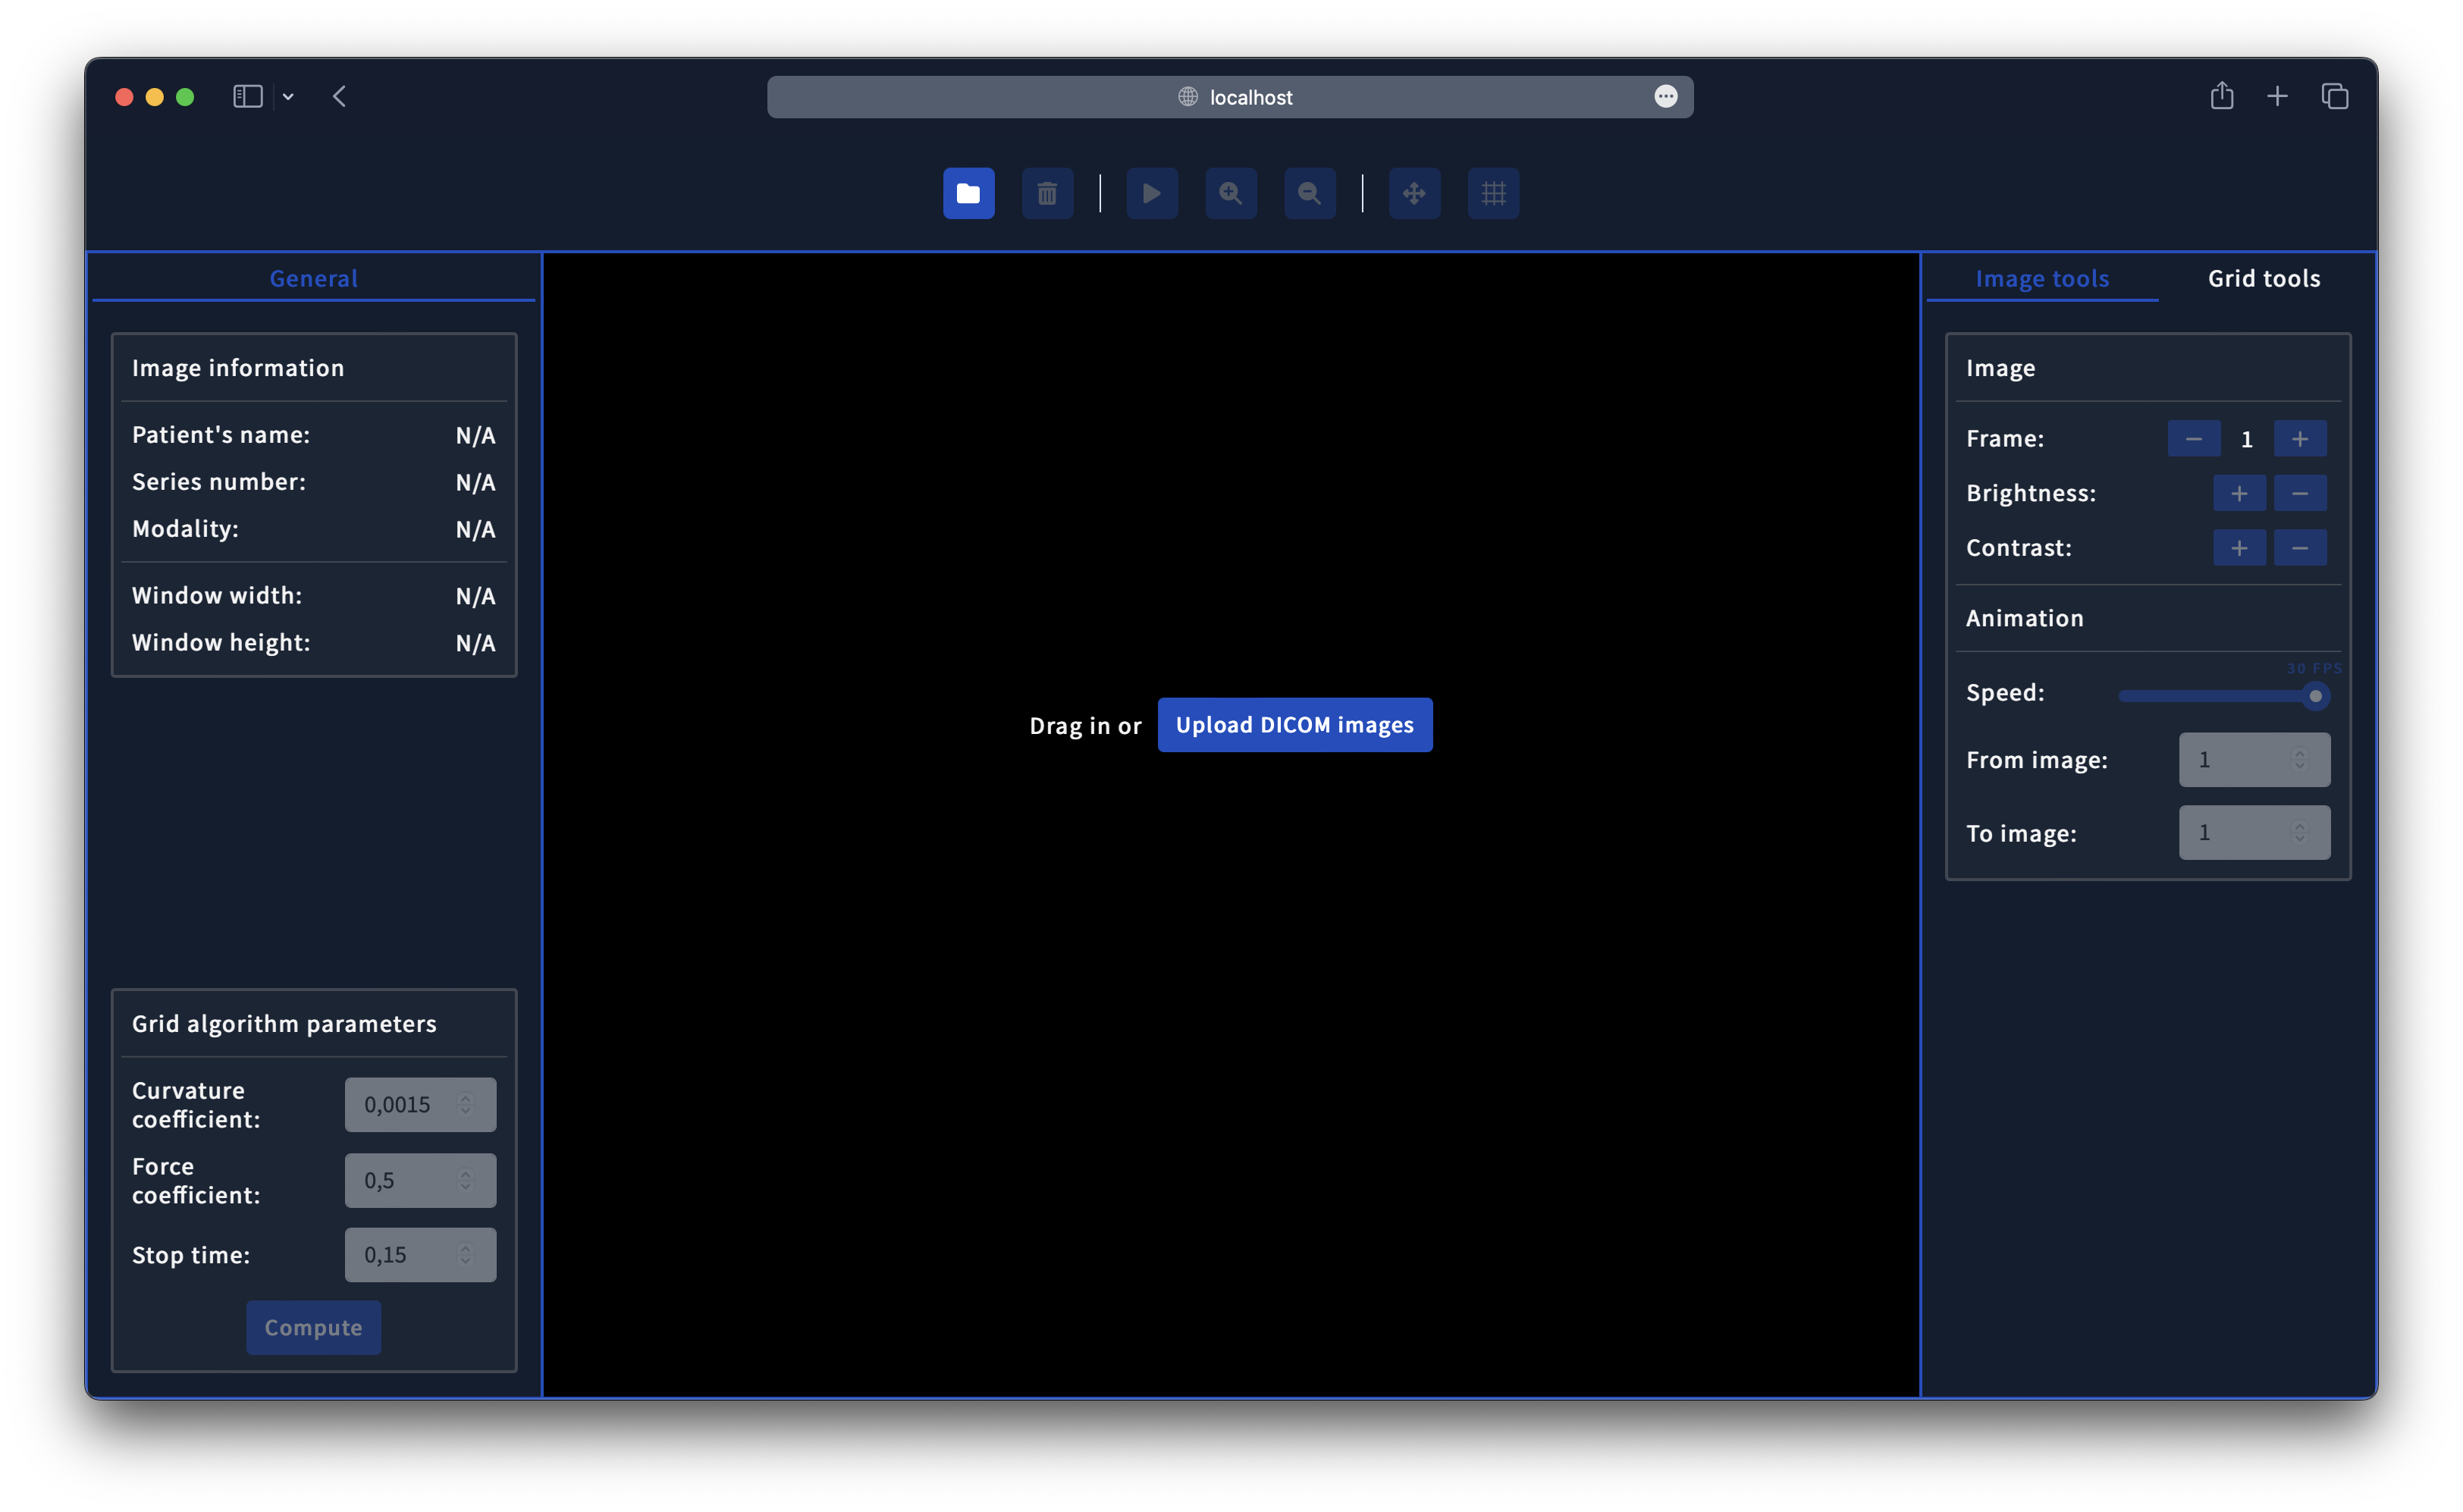
\includegraphics[height=9cm]{media/new_app/initial_state.png}
        \captionsetup{justification=centering}
        \captionof{figure}{Snímka zobrazujúca počiatočný stav aplikácie po jej načítaní.}
\end {figure}

\begin {figure}[H]
        \centering
        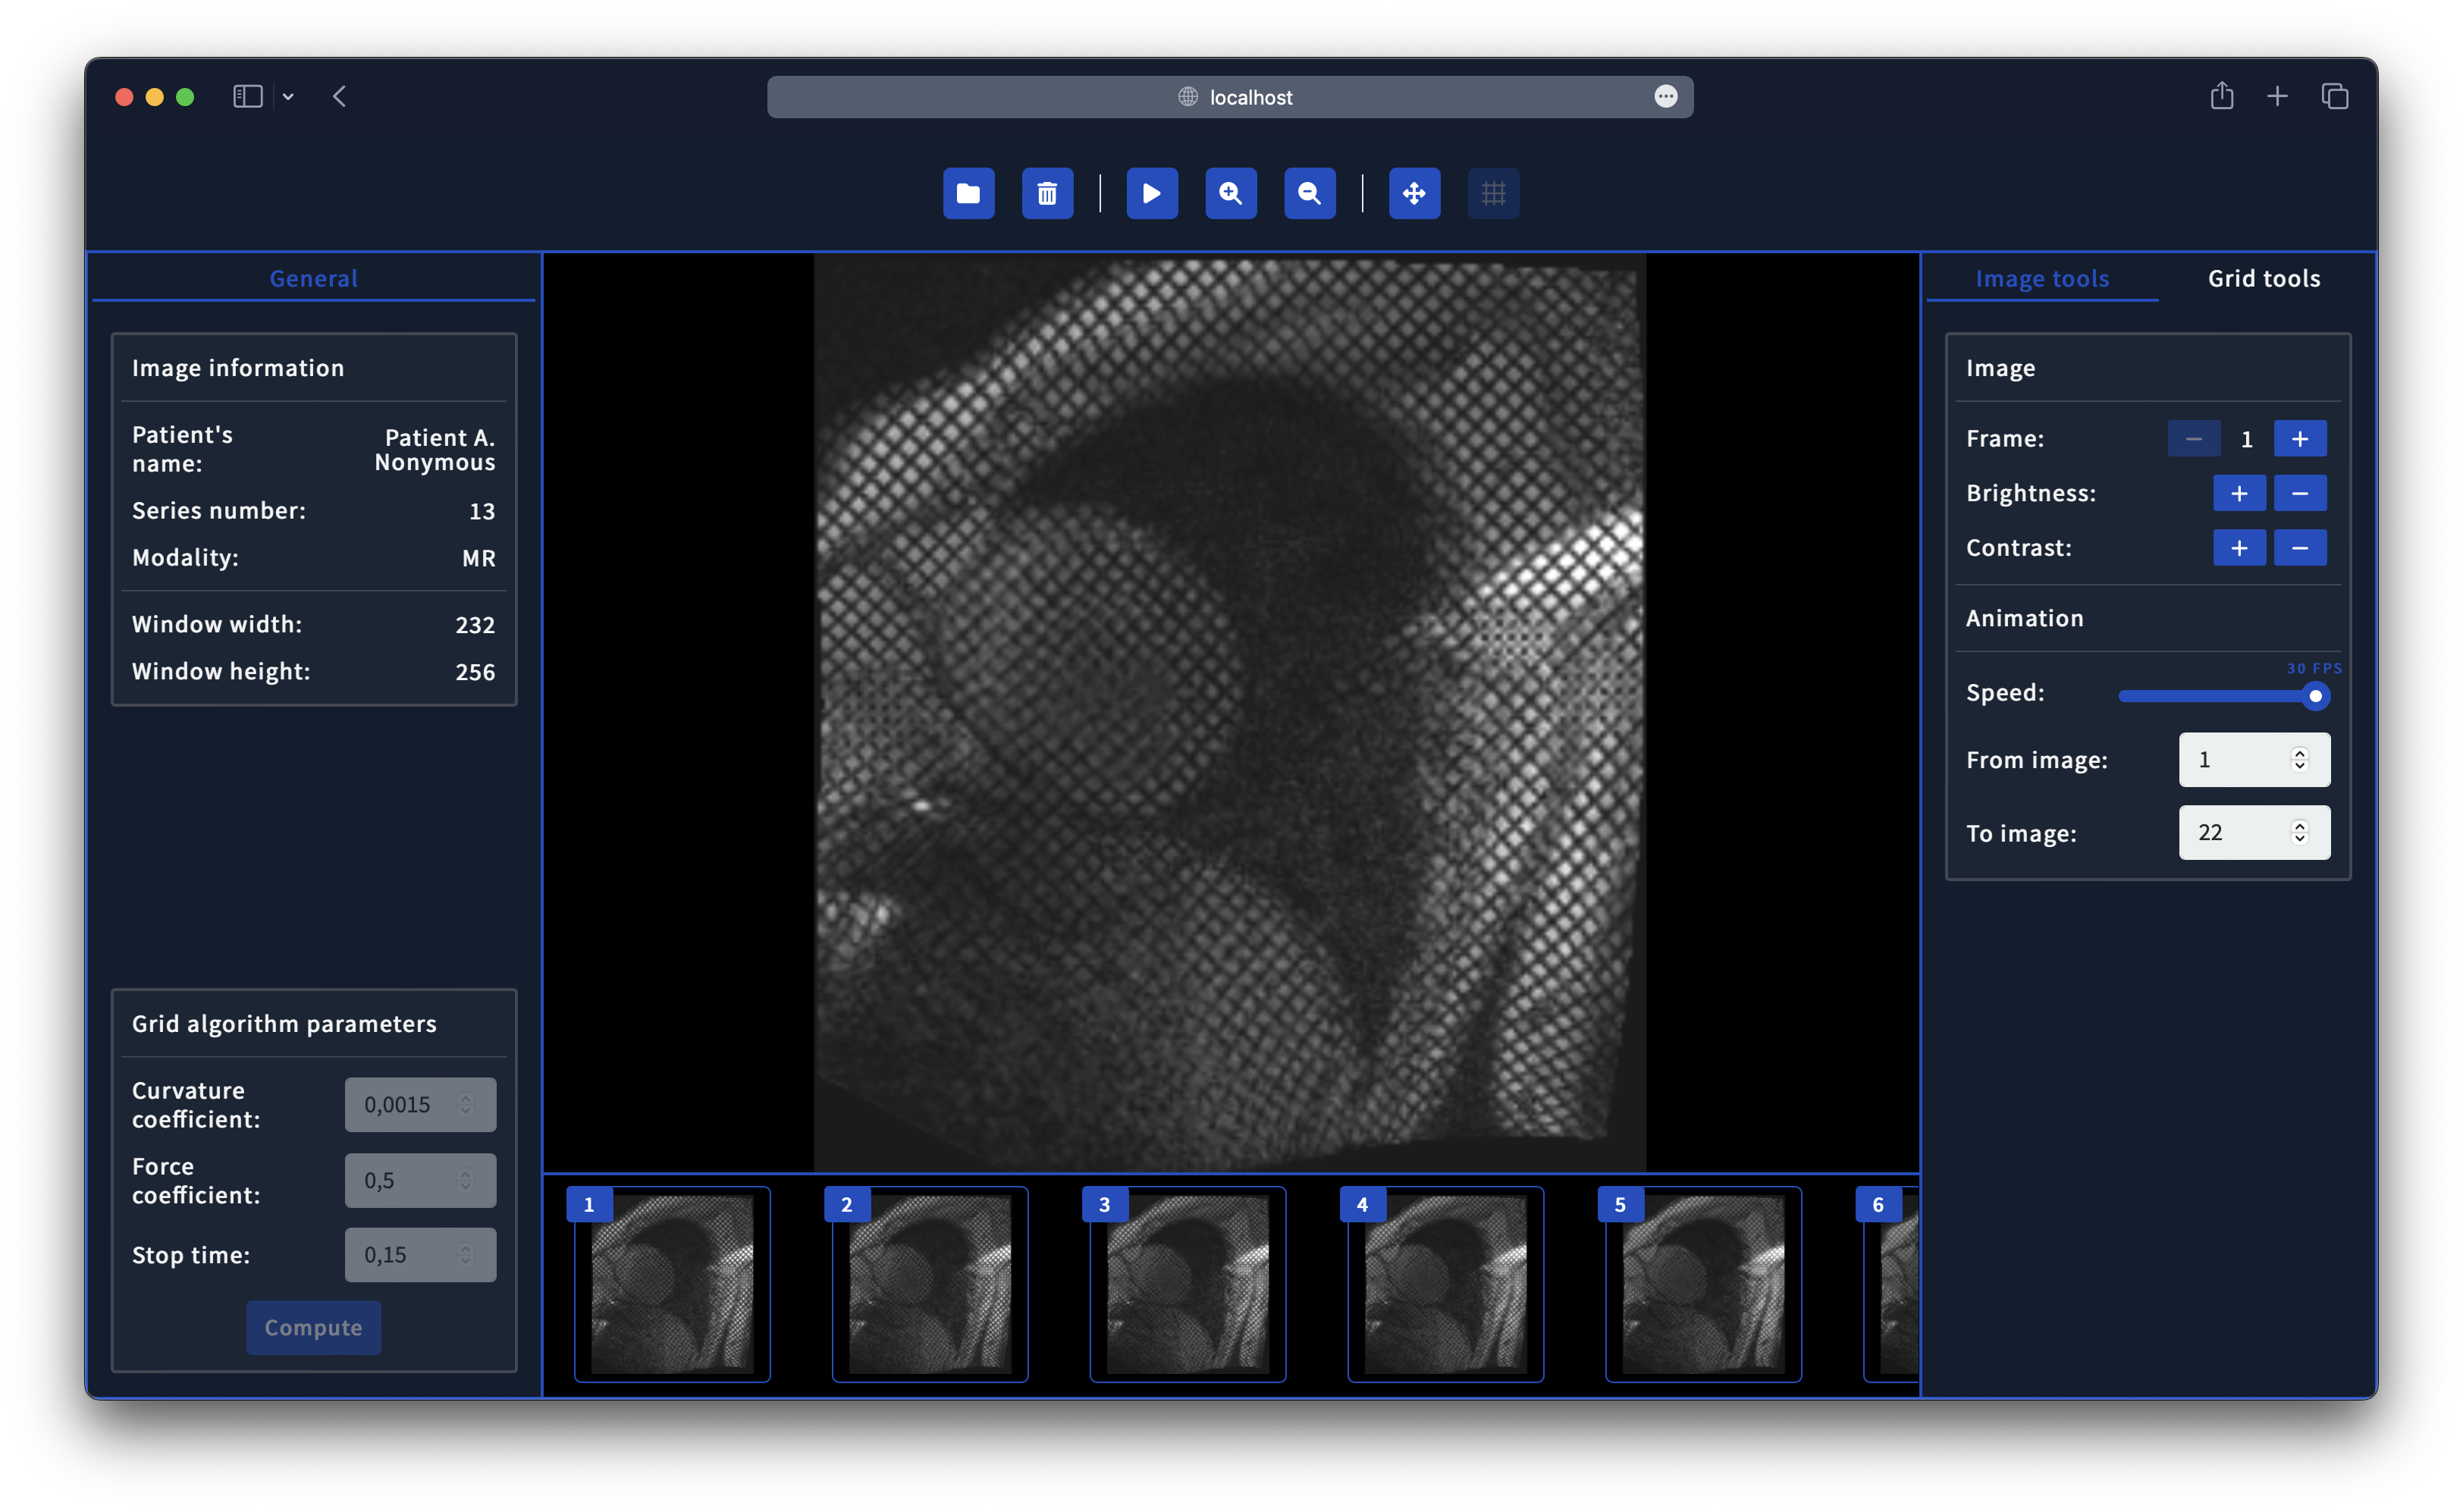
\includegraphics[height=9cm]{media/new_app/state_after_import.png}
        \captionsetup{justification=centering}
        \captionof{figure}{Snímka zobrazujúca stav aplikácie po importovaní DICOM snímiek.}
\end {figure}

\begin {figure}[H]
        \centering
        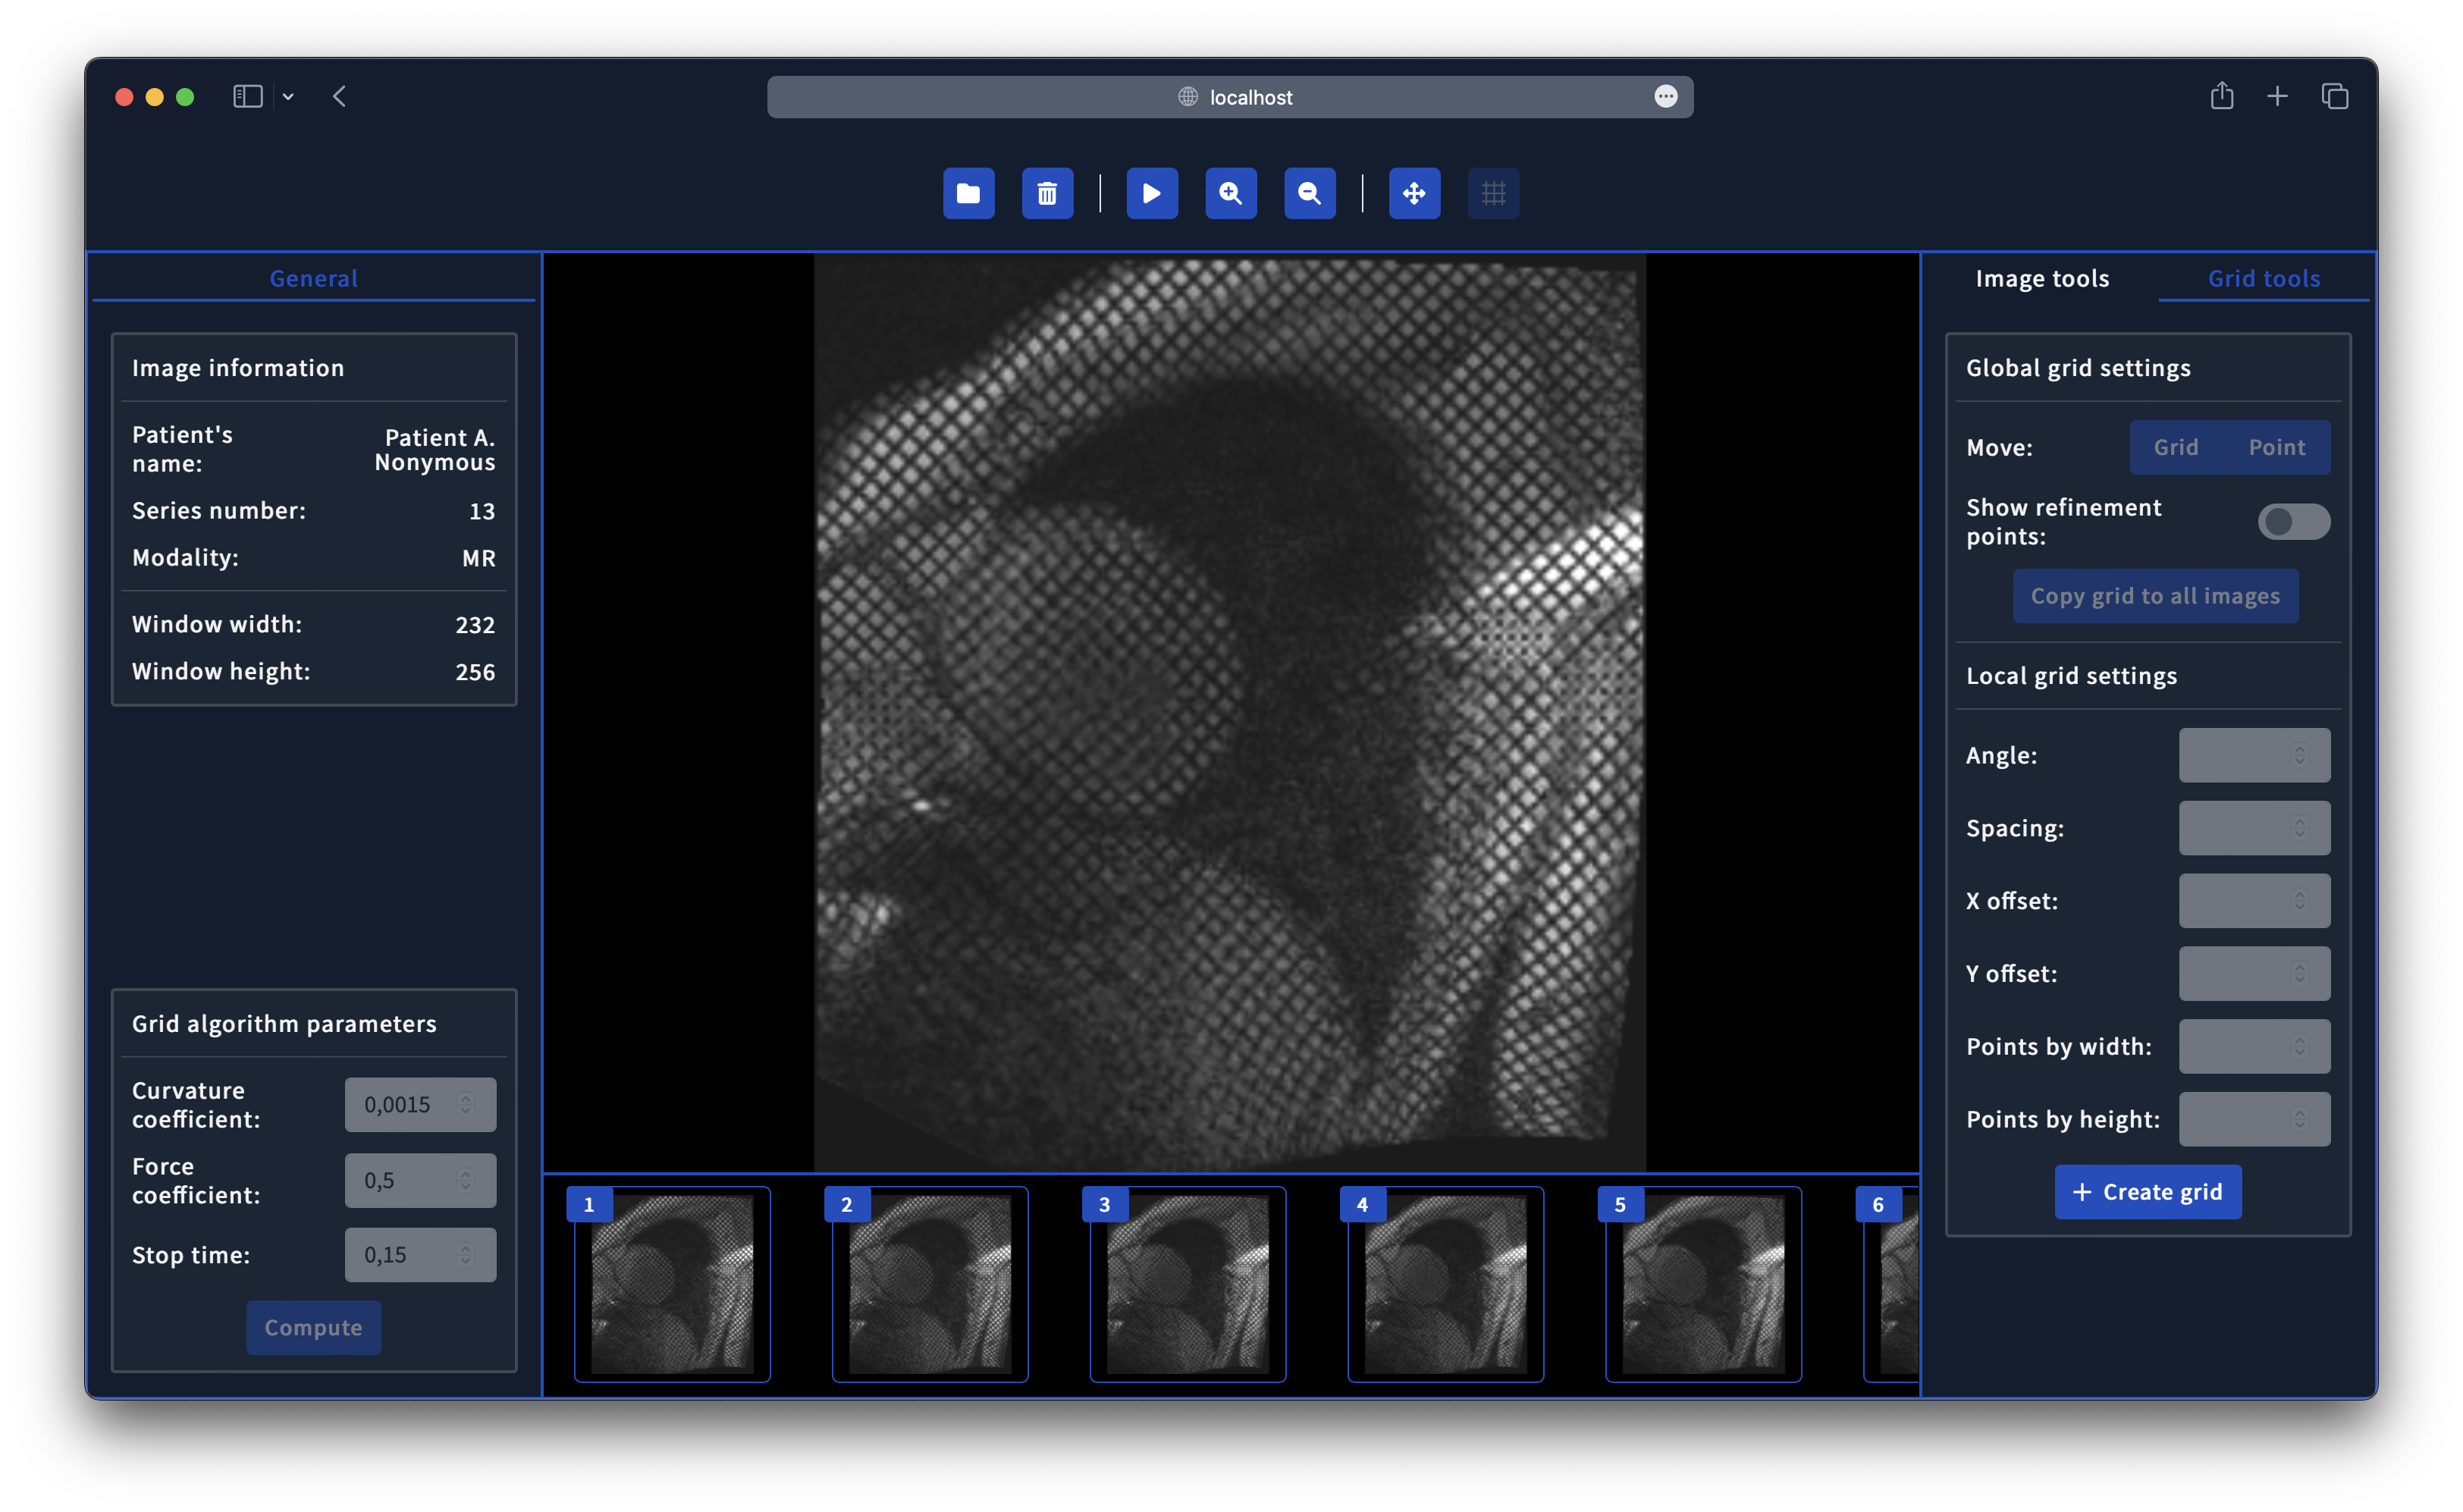
\includegraphics[height=9cm]{media/new_app/grid_tools.png}
        \captionsetup{justification=centering}
        \captionof{figure}{Snímka zobrazujúca kartu \uv{Grid tool} v pravom postrannom paneli.}
\end {figure}

\begin {figure}[H]
        \centering
        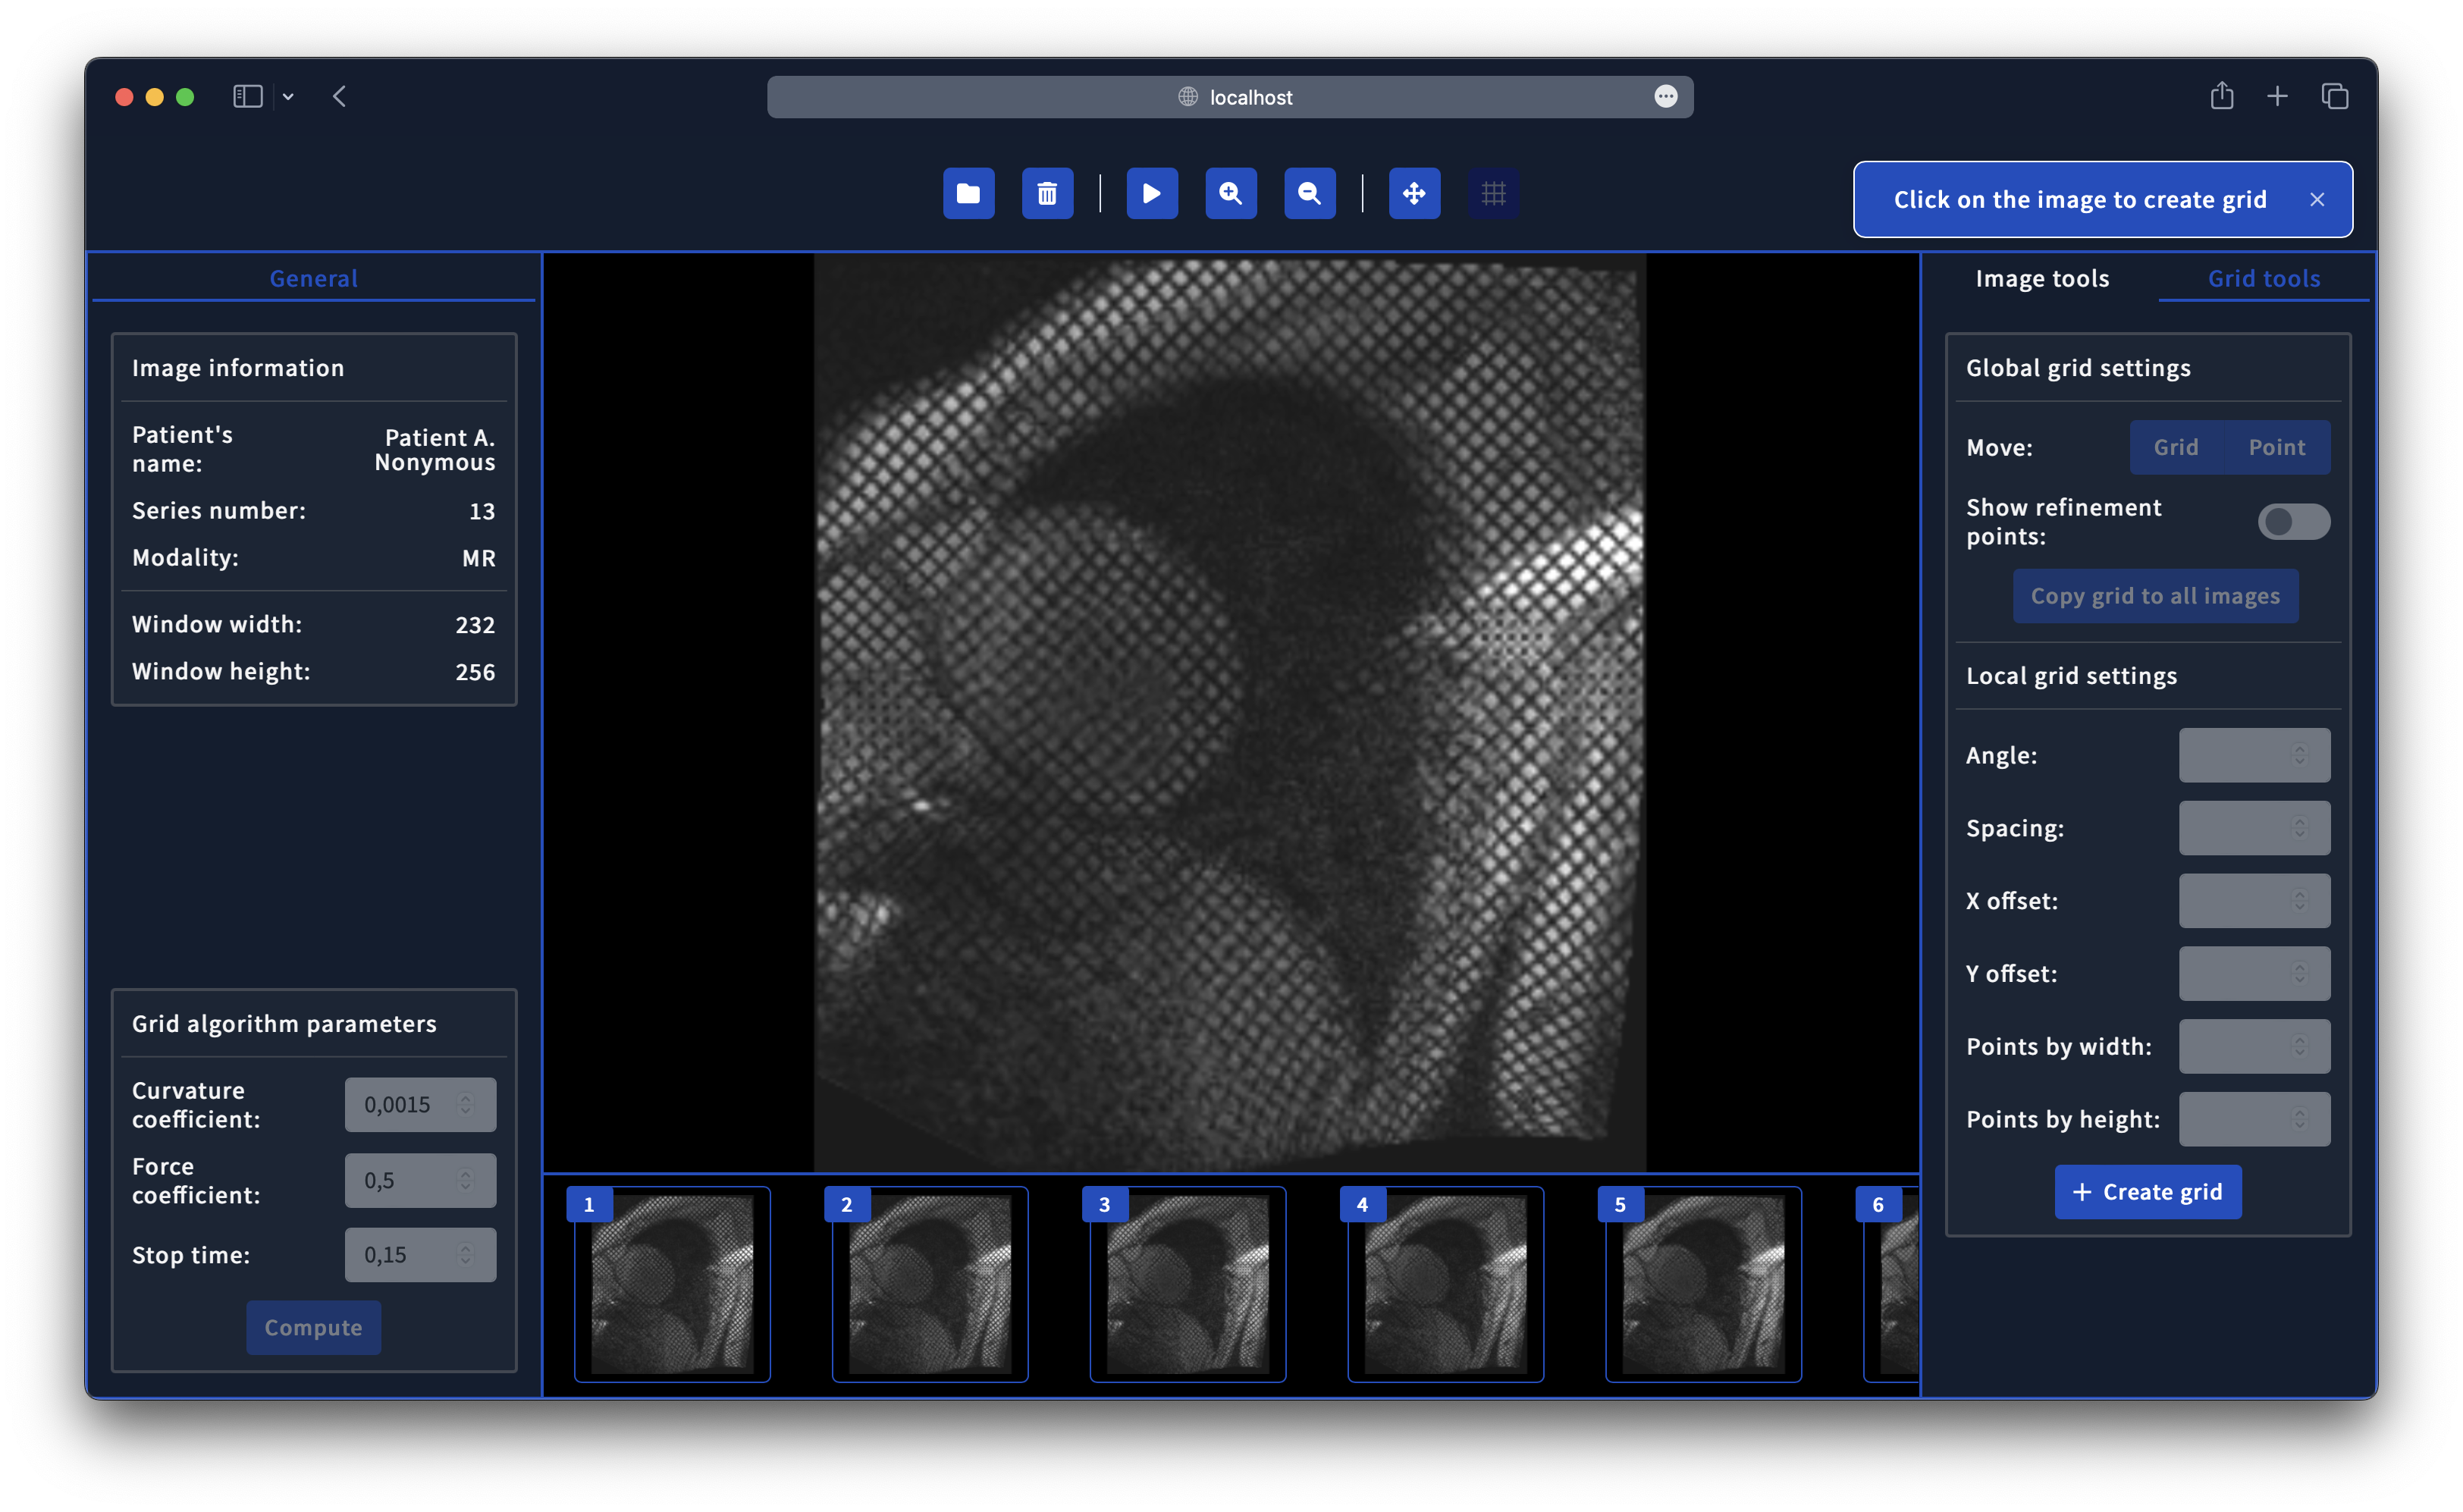
\includegraphics[height=9cm]{media/new_app/notification.png}
        \captionsetup{justification=centering}
        \captionof{figure}{Snímka zobrazujúca notifikáciu aplikácie s krokom pre vytvorenie mriežky.}
\end {figure}

\begin {figure}[H]
        \centering
        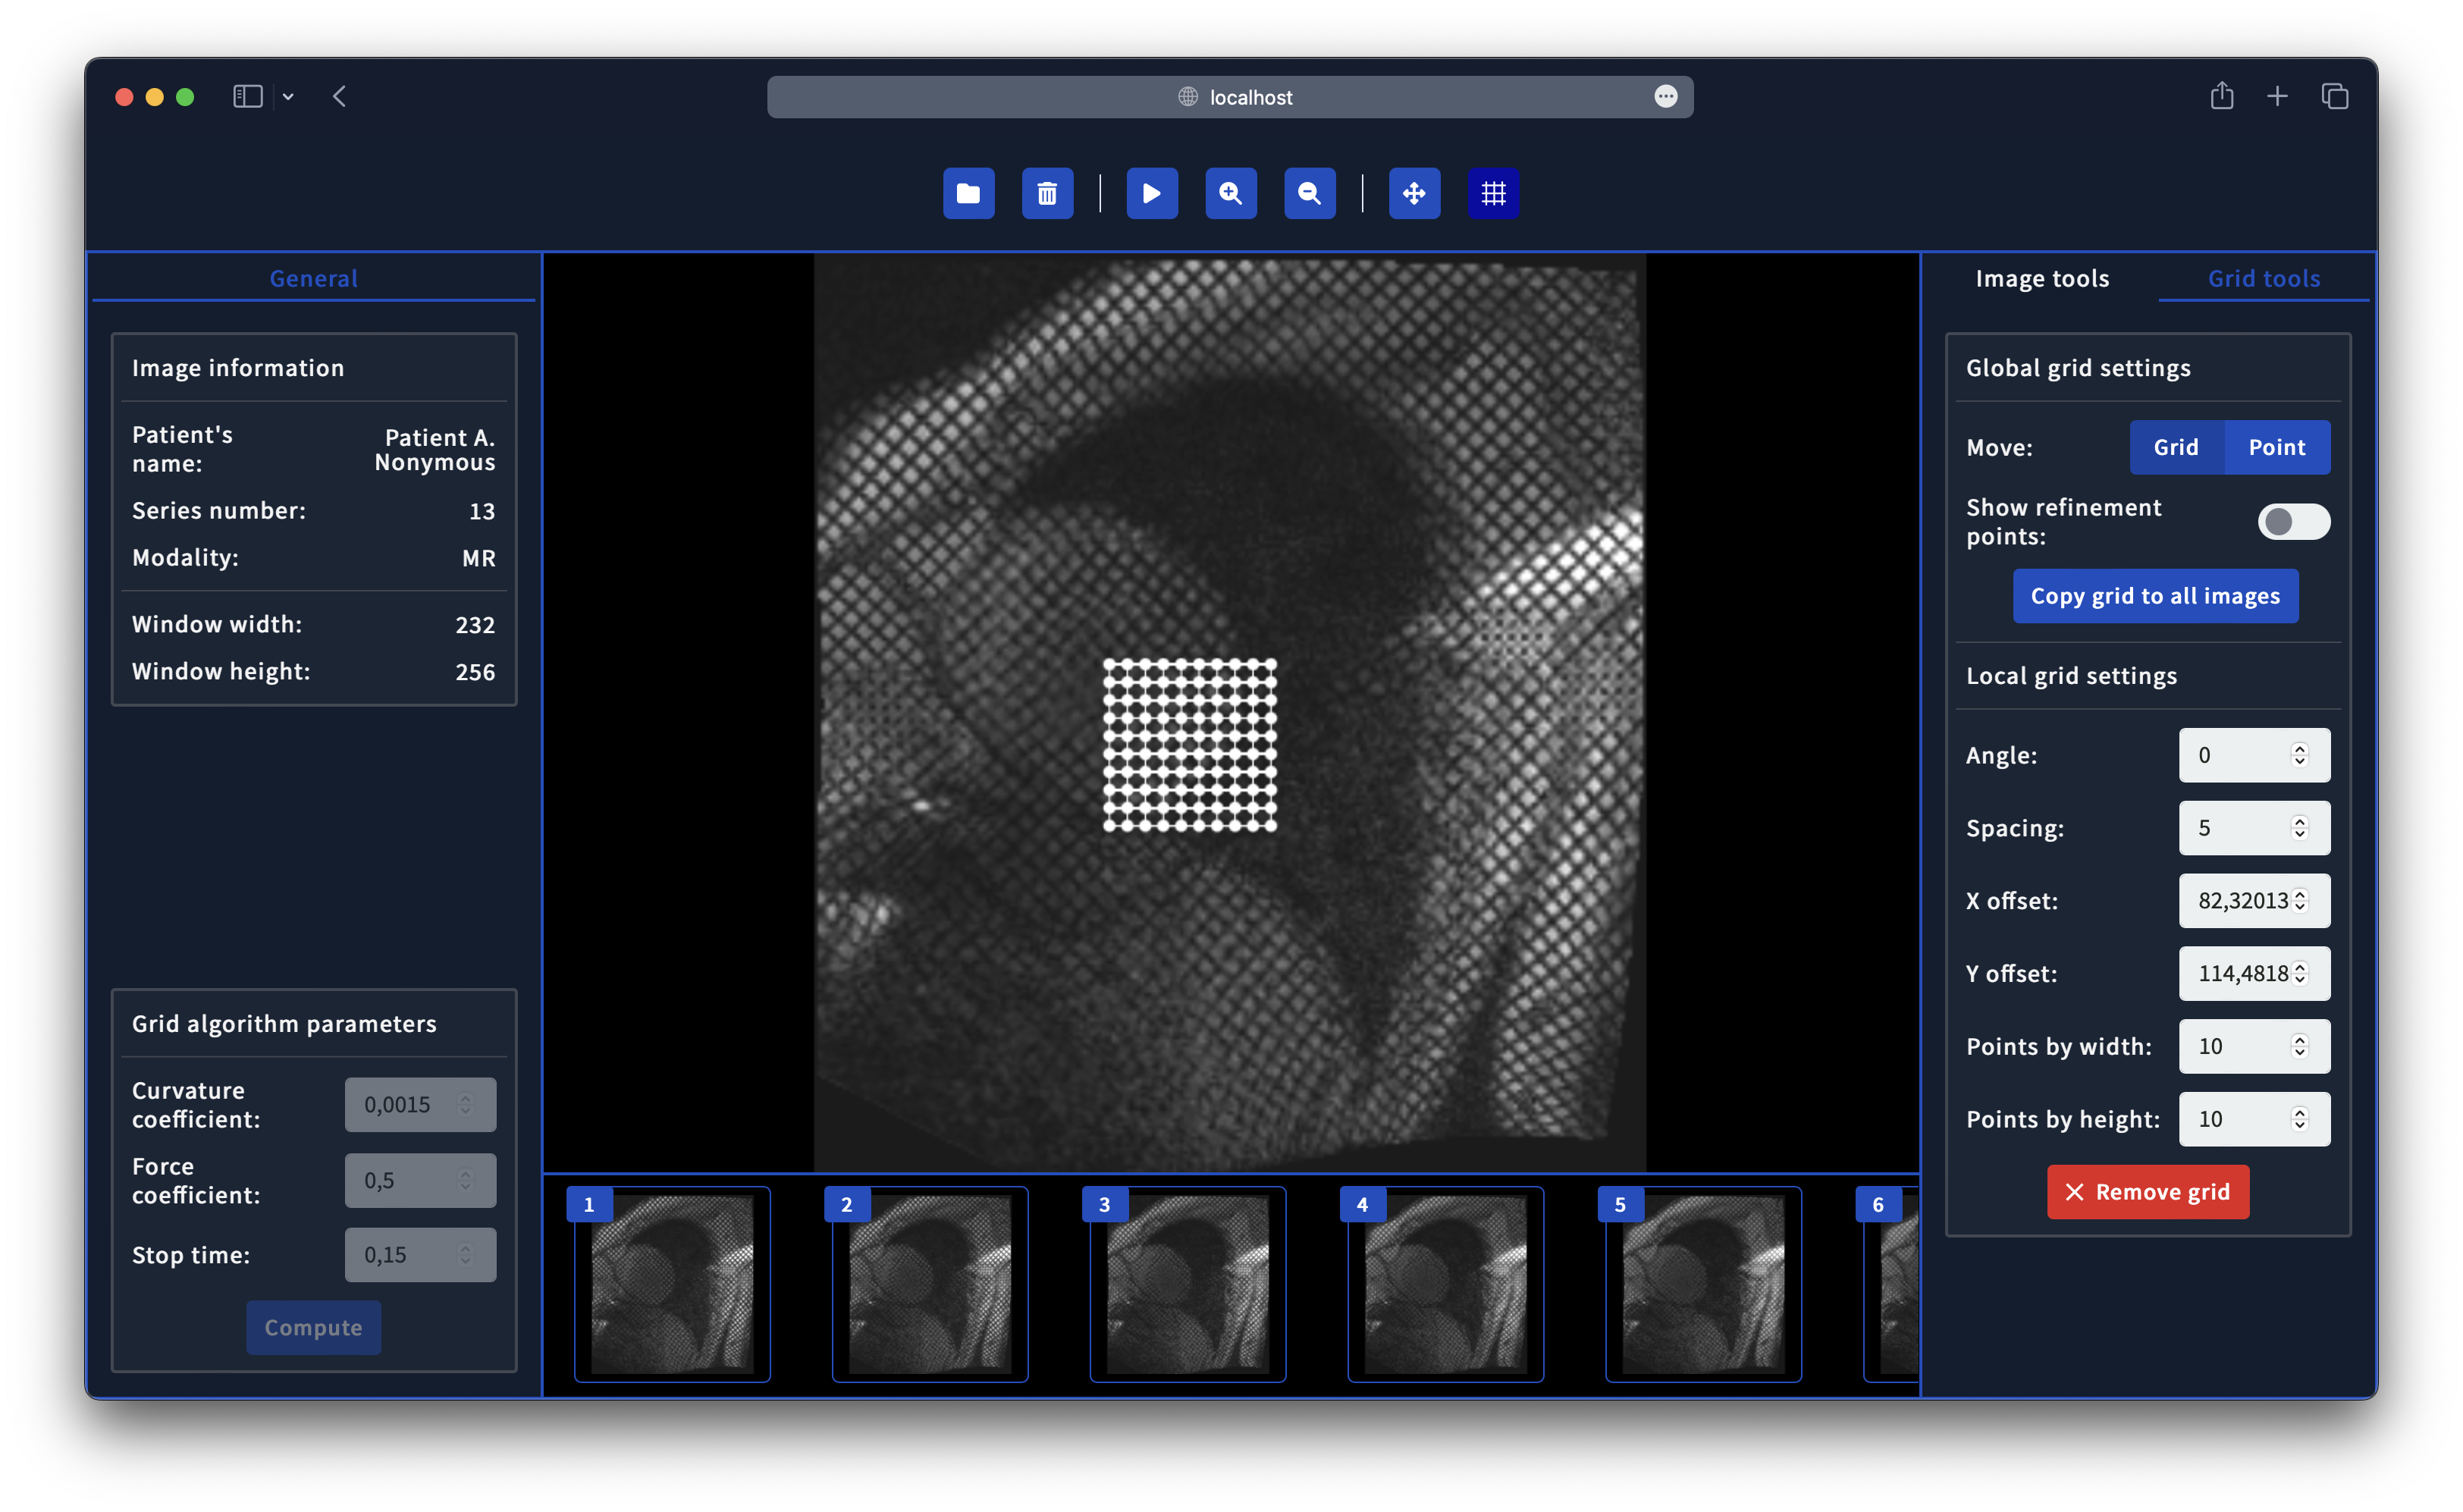
\includegraphics[height=9cm]{media/new_app/grid.png}
        \captionsetup{justification=centering}
        \captionof{figure}{Snímka zobrazujúca vygenerovanú mriežku zobrazenú nad DICOM snímkou.}
\end {figure}

\begin {figure}[H]
        \centering
        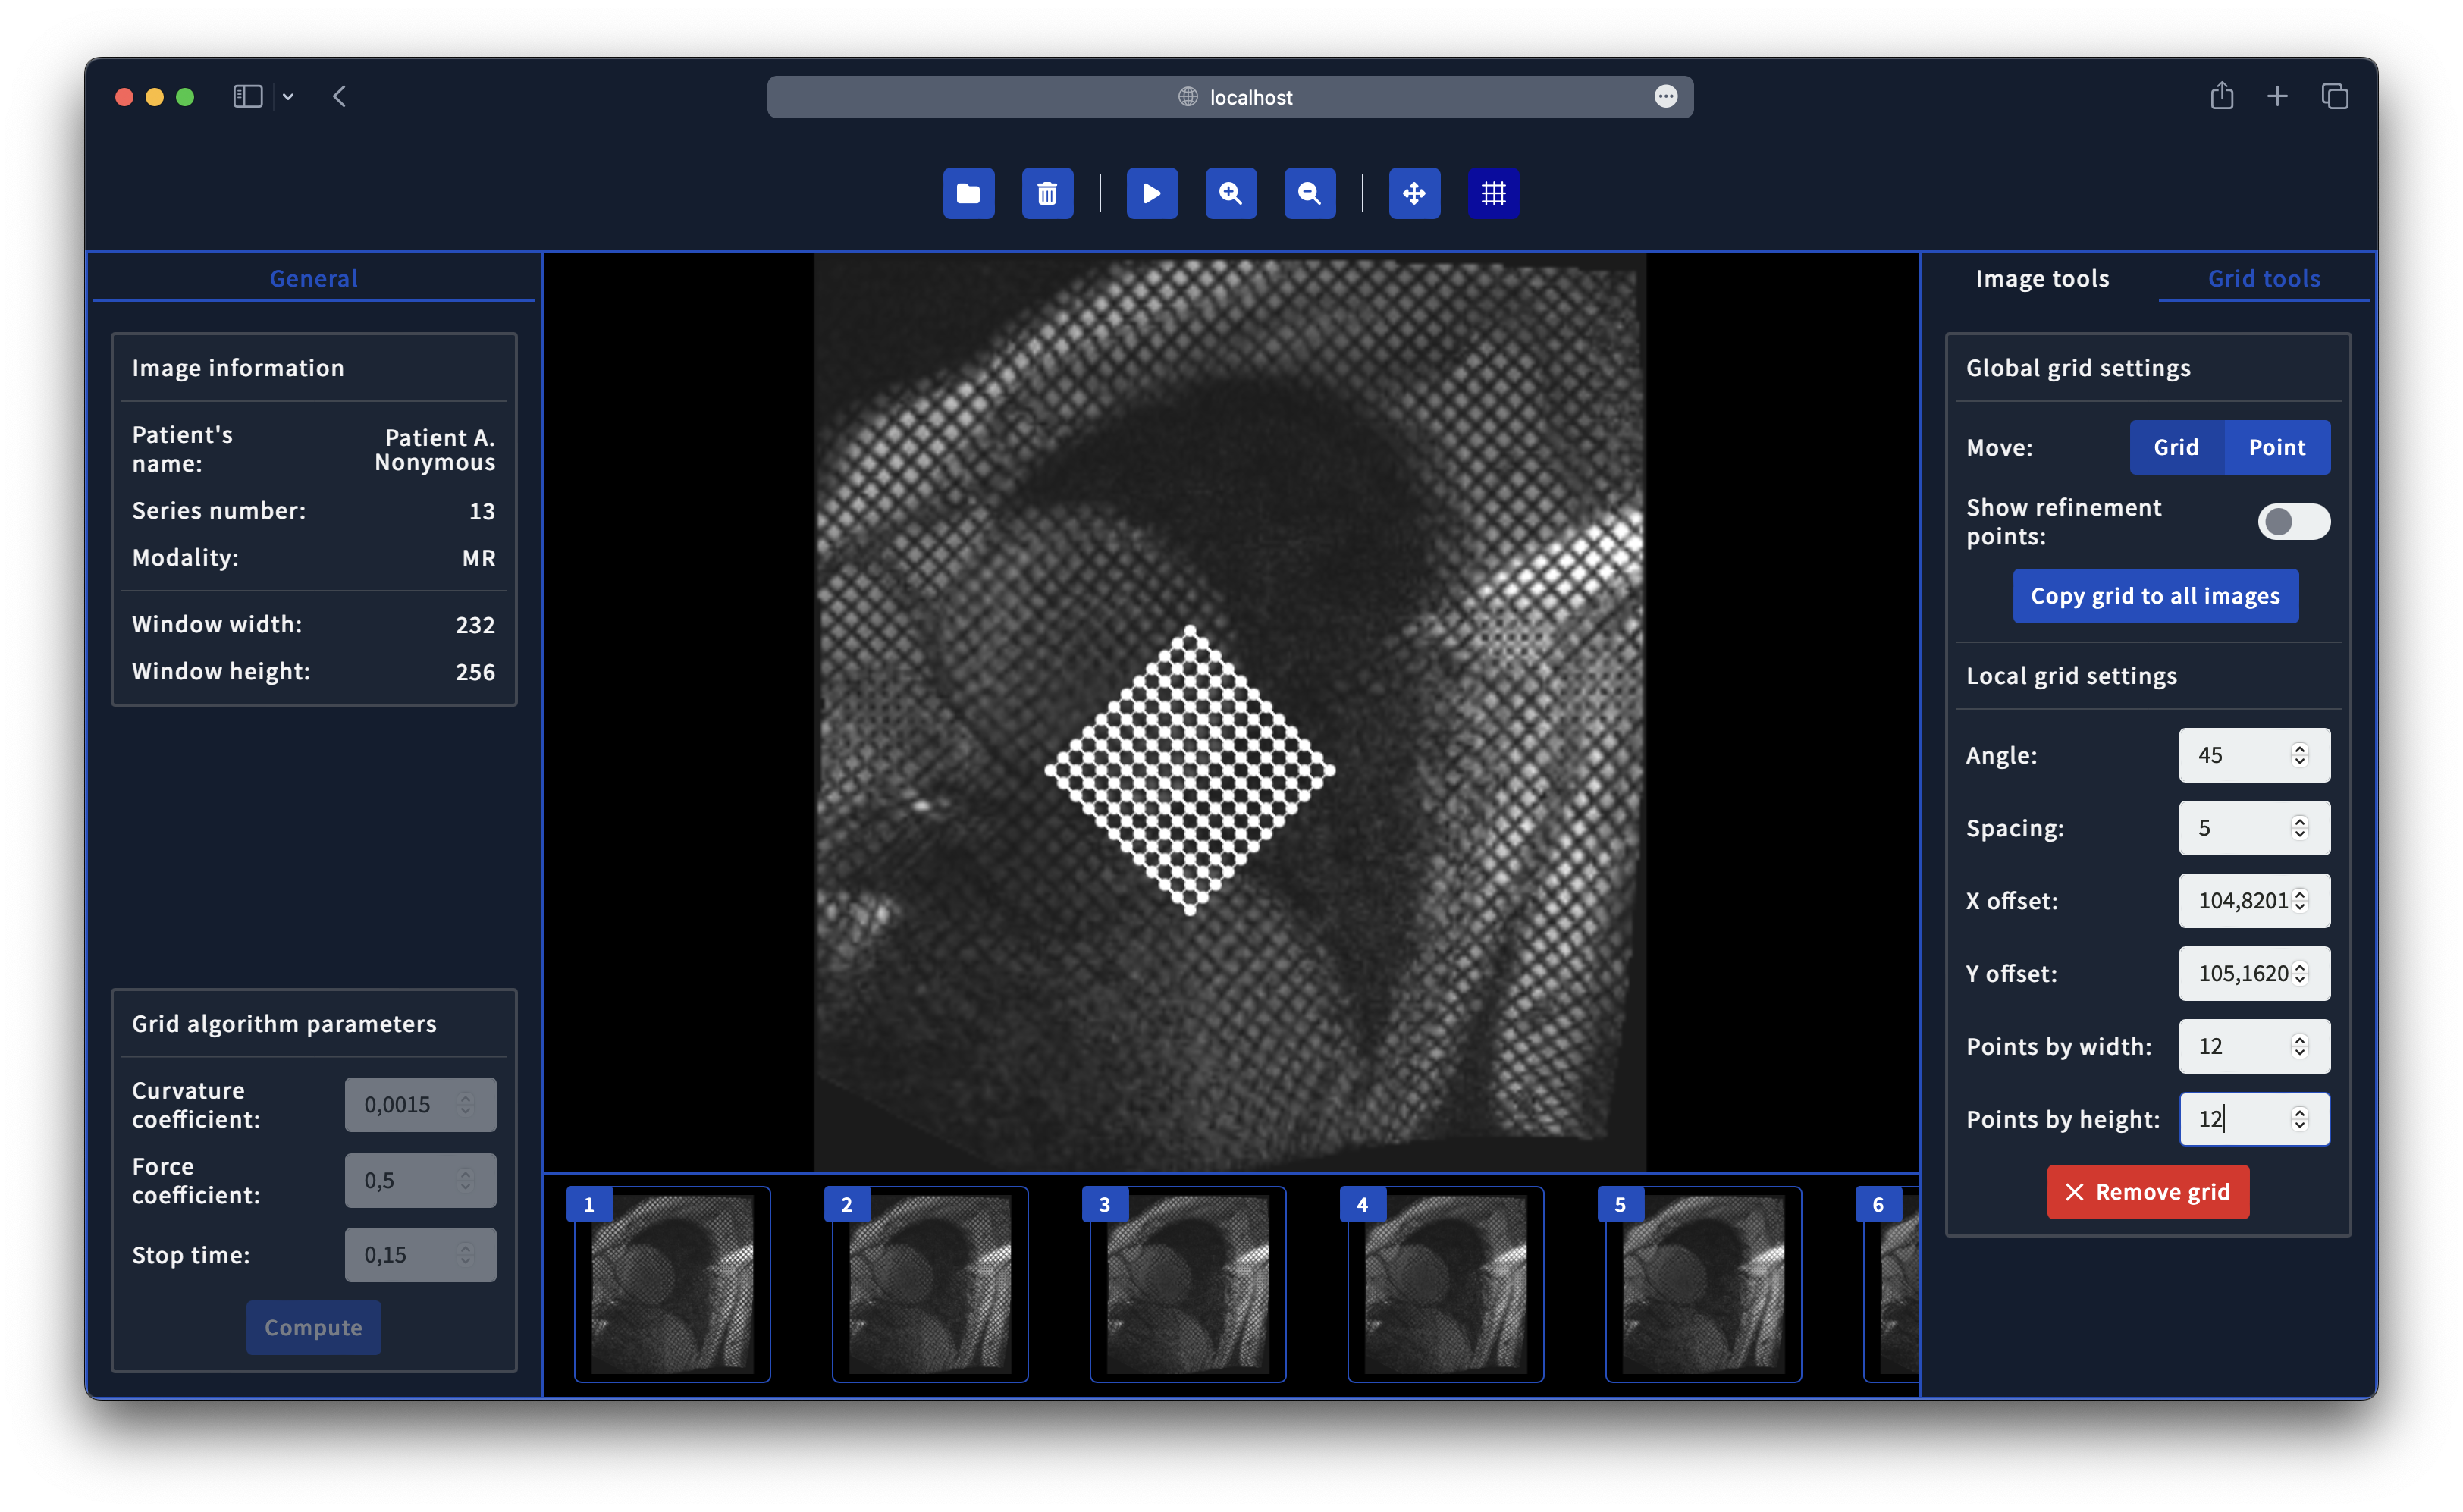
\includegraphics[height=9cm]{media/new_app/grid_modification.png}
        \captionsetup{justification=centering}
        \captionof{figure}{Snímka zobrazujúca zmenu štruktúry mriežky na základe zmenených parametrov.}
\end {figure}

\begin {figure}[H]
        \centering
        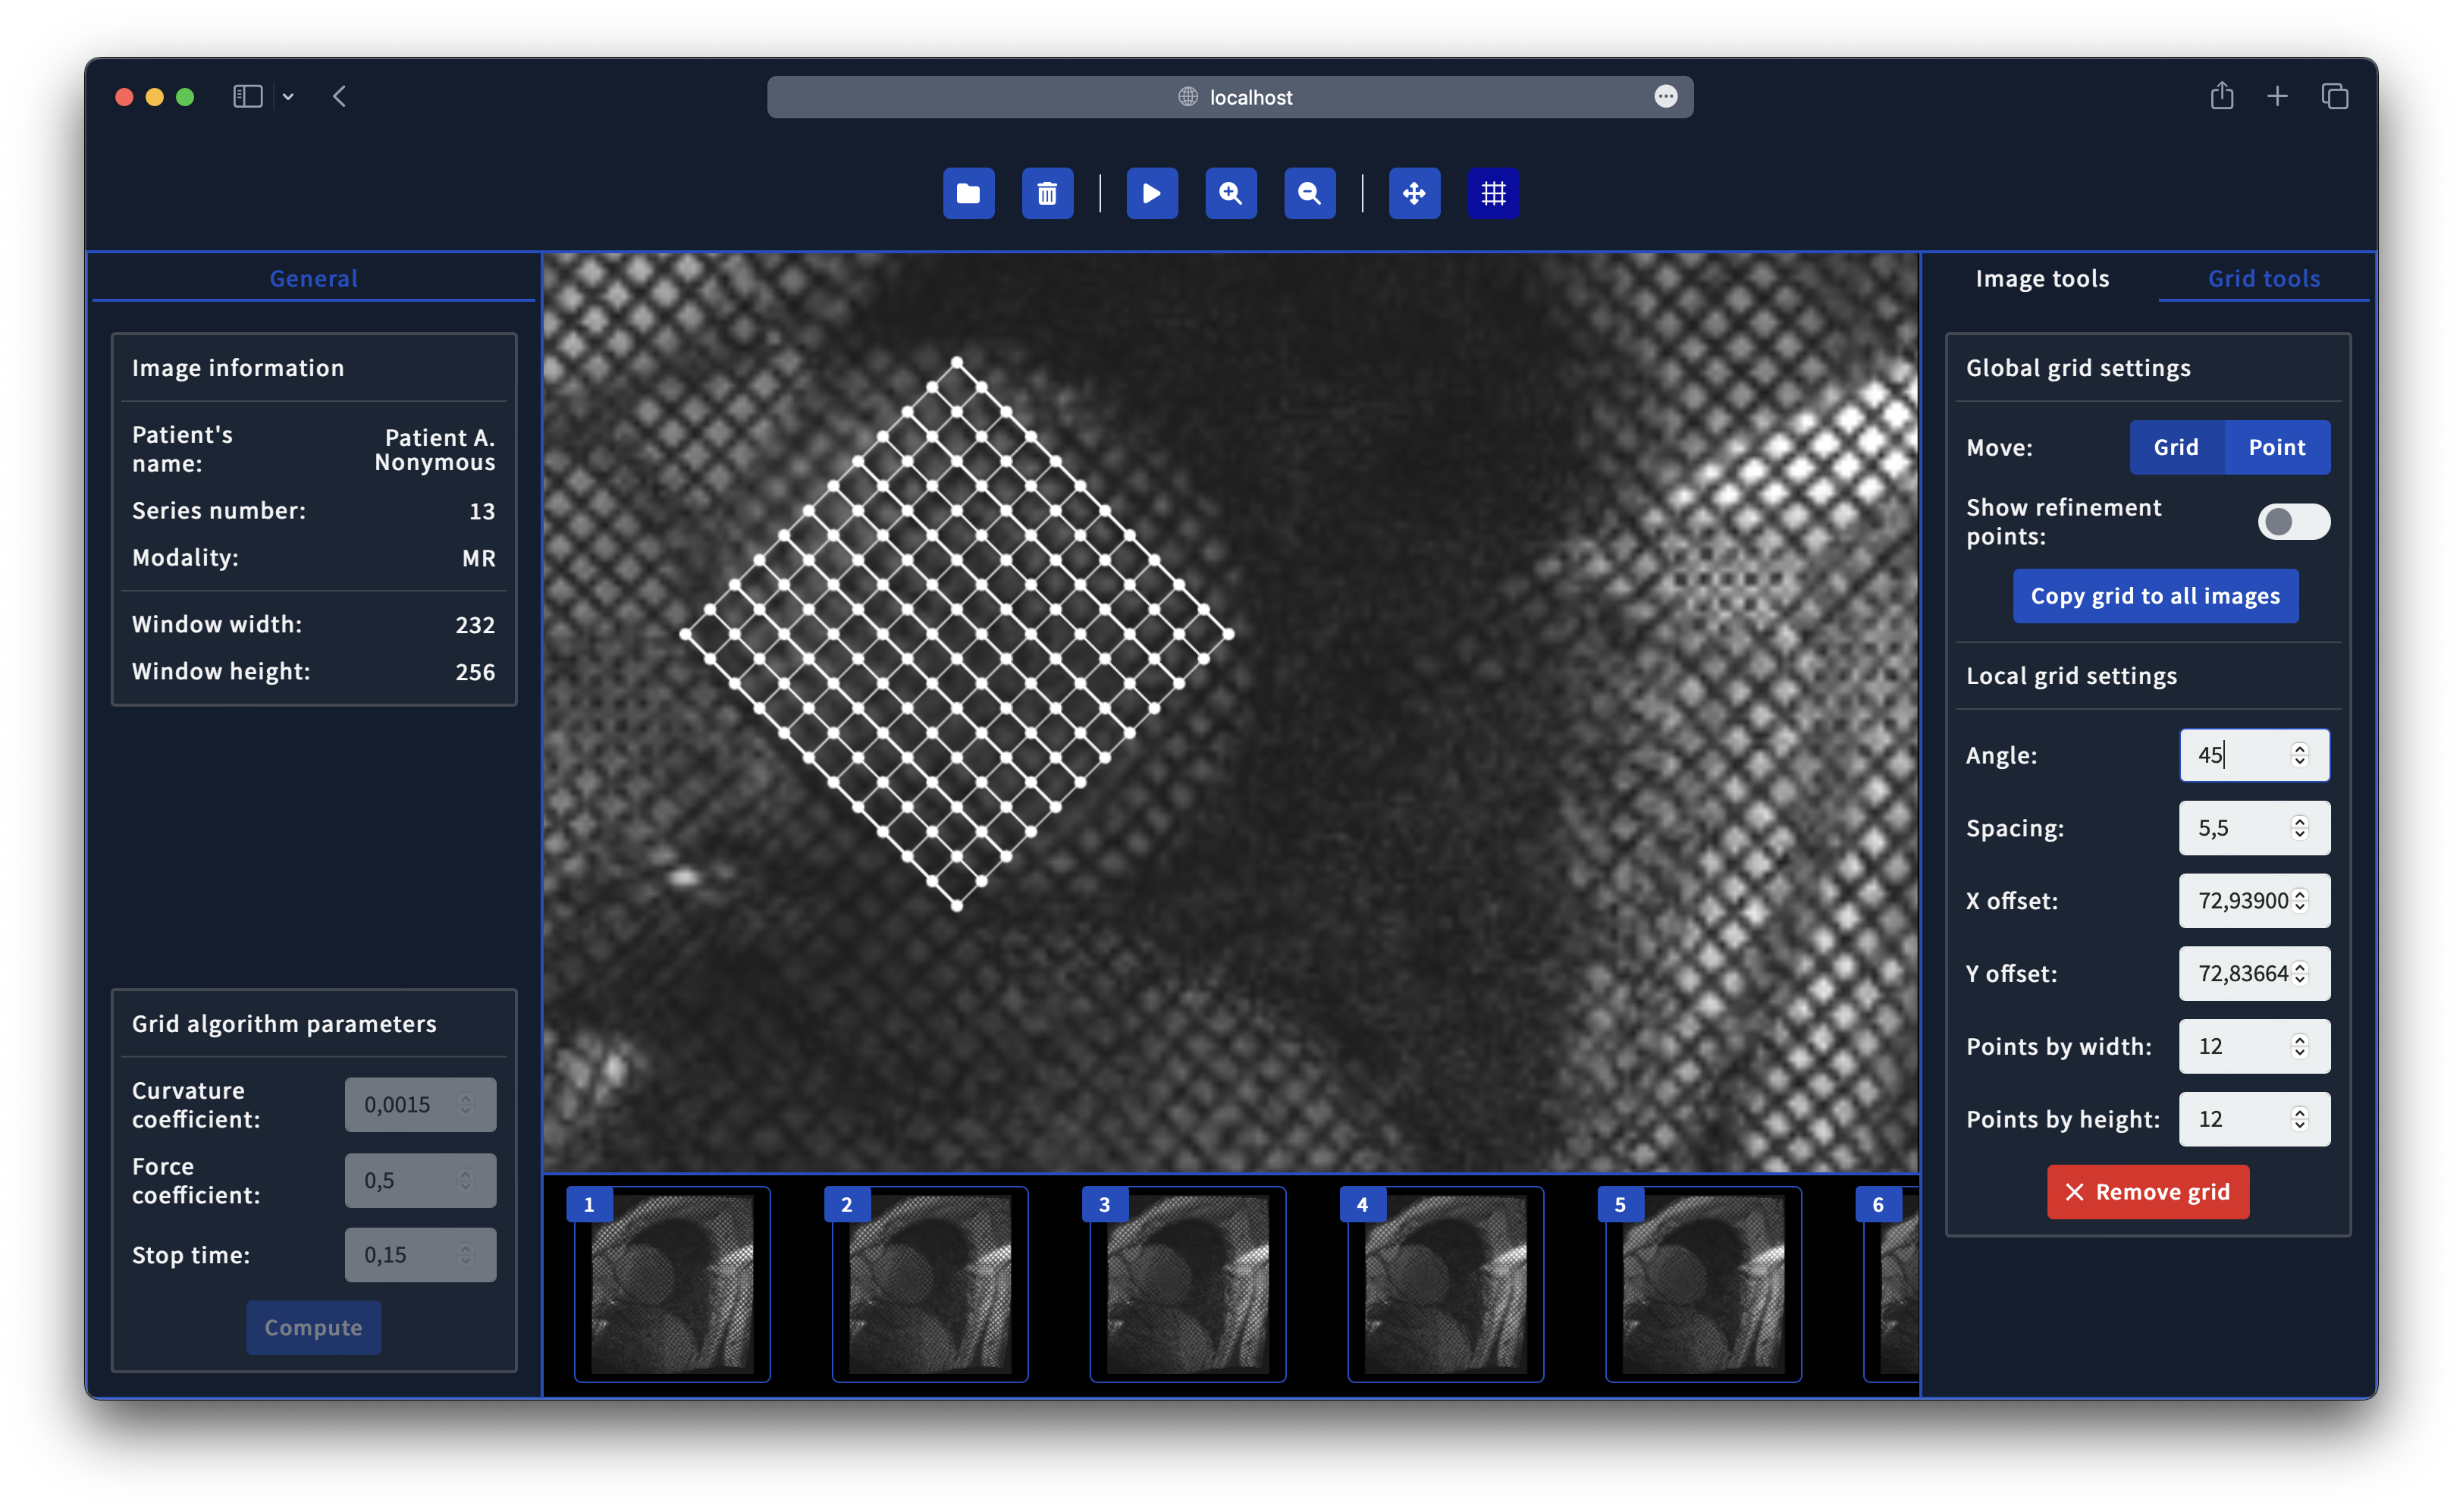
\includegraphics[height=9cm]{media/new_app/zoomed_in.png}
        \captionsetup{justification=centering}
        \captionof{figure}{Snímka zobrazujúca priblíženú DICOM snímku.}
\end {figure}

\begin {figure}[H]
        \centering
        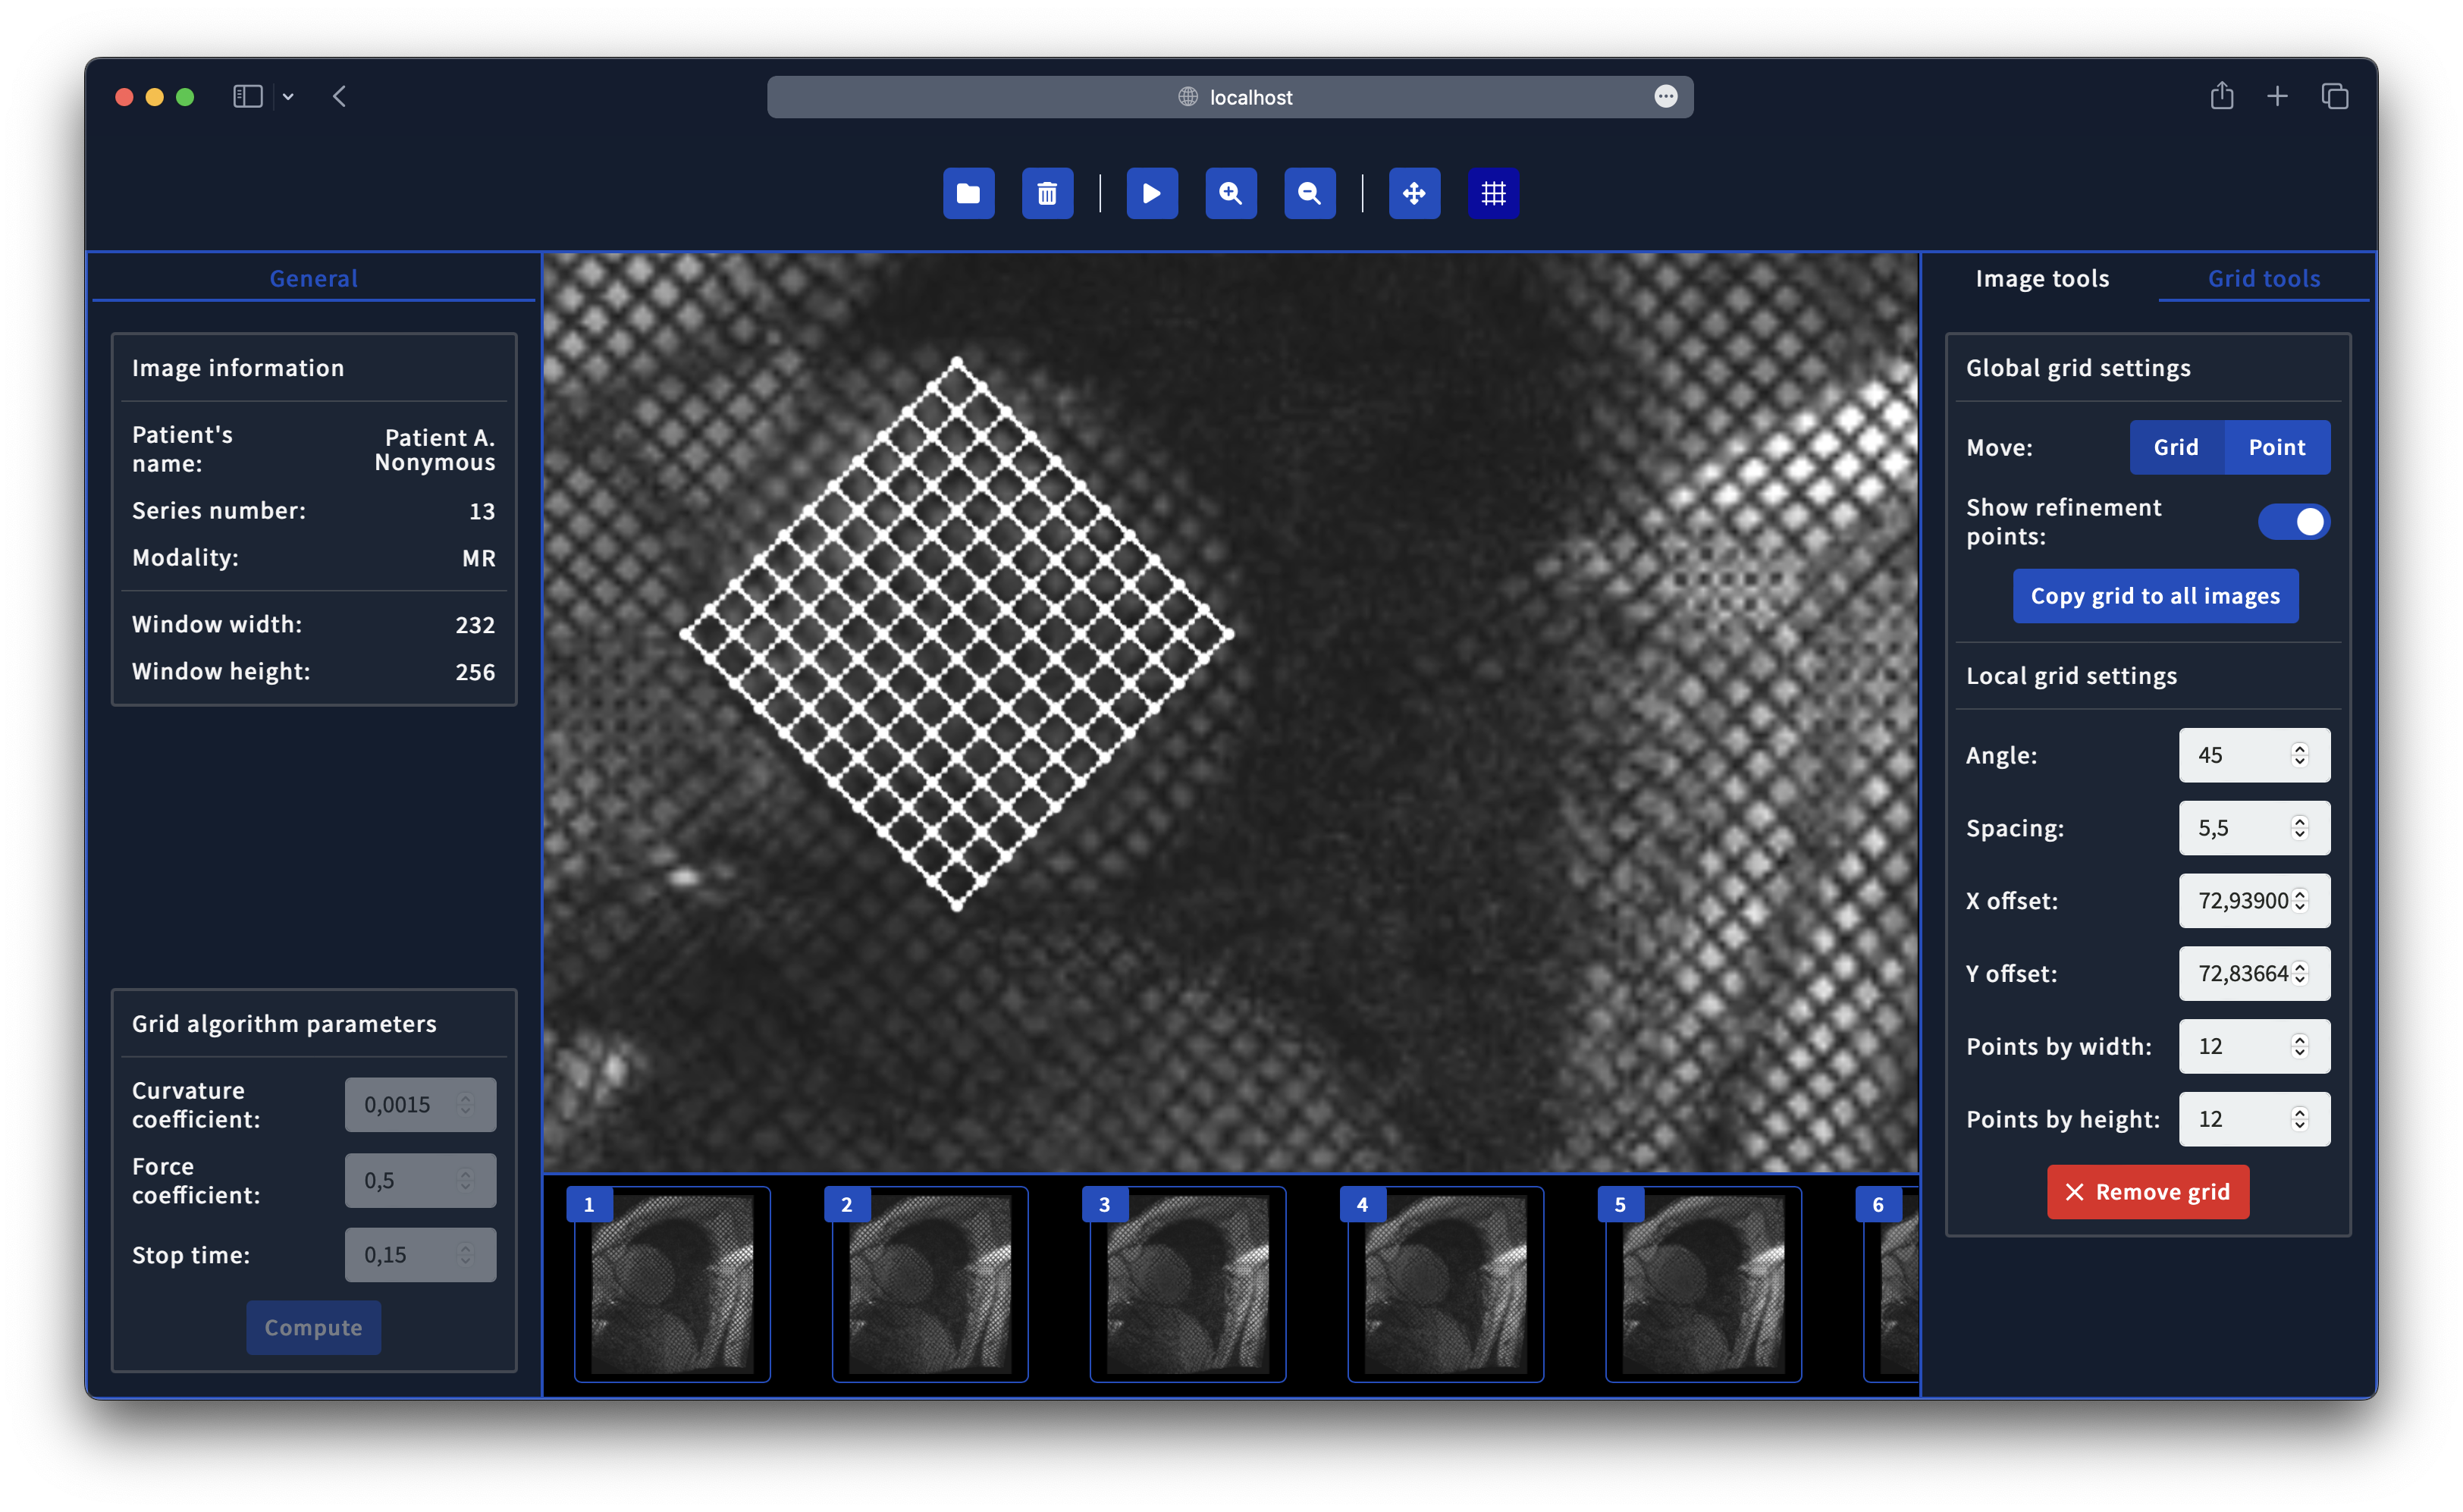
\includegraphics[height=9cm]{media/new_app/refinement_points_on.png}
        \captionsetup{justification=centering}
        \captionof{figure}{Snímka zobrazujúca \uv{refinement} body mriežky.}
\end {figure}

\begin {figure}[H]
        \centering
        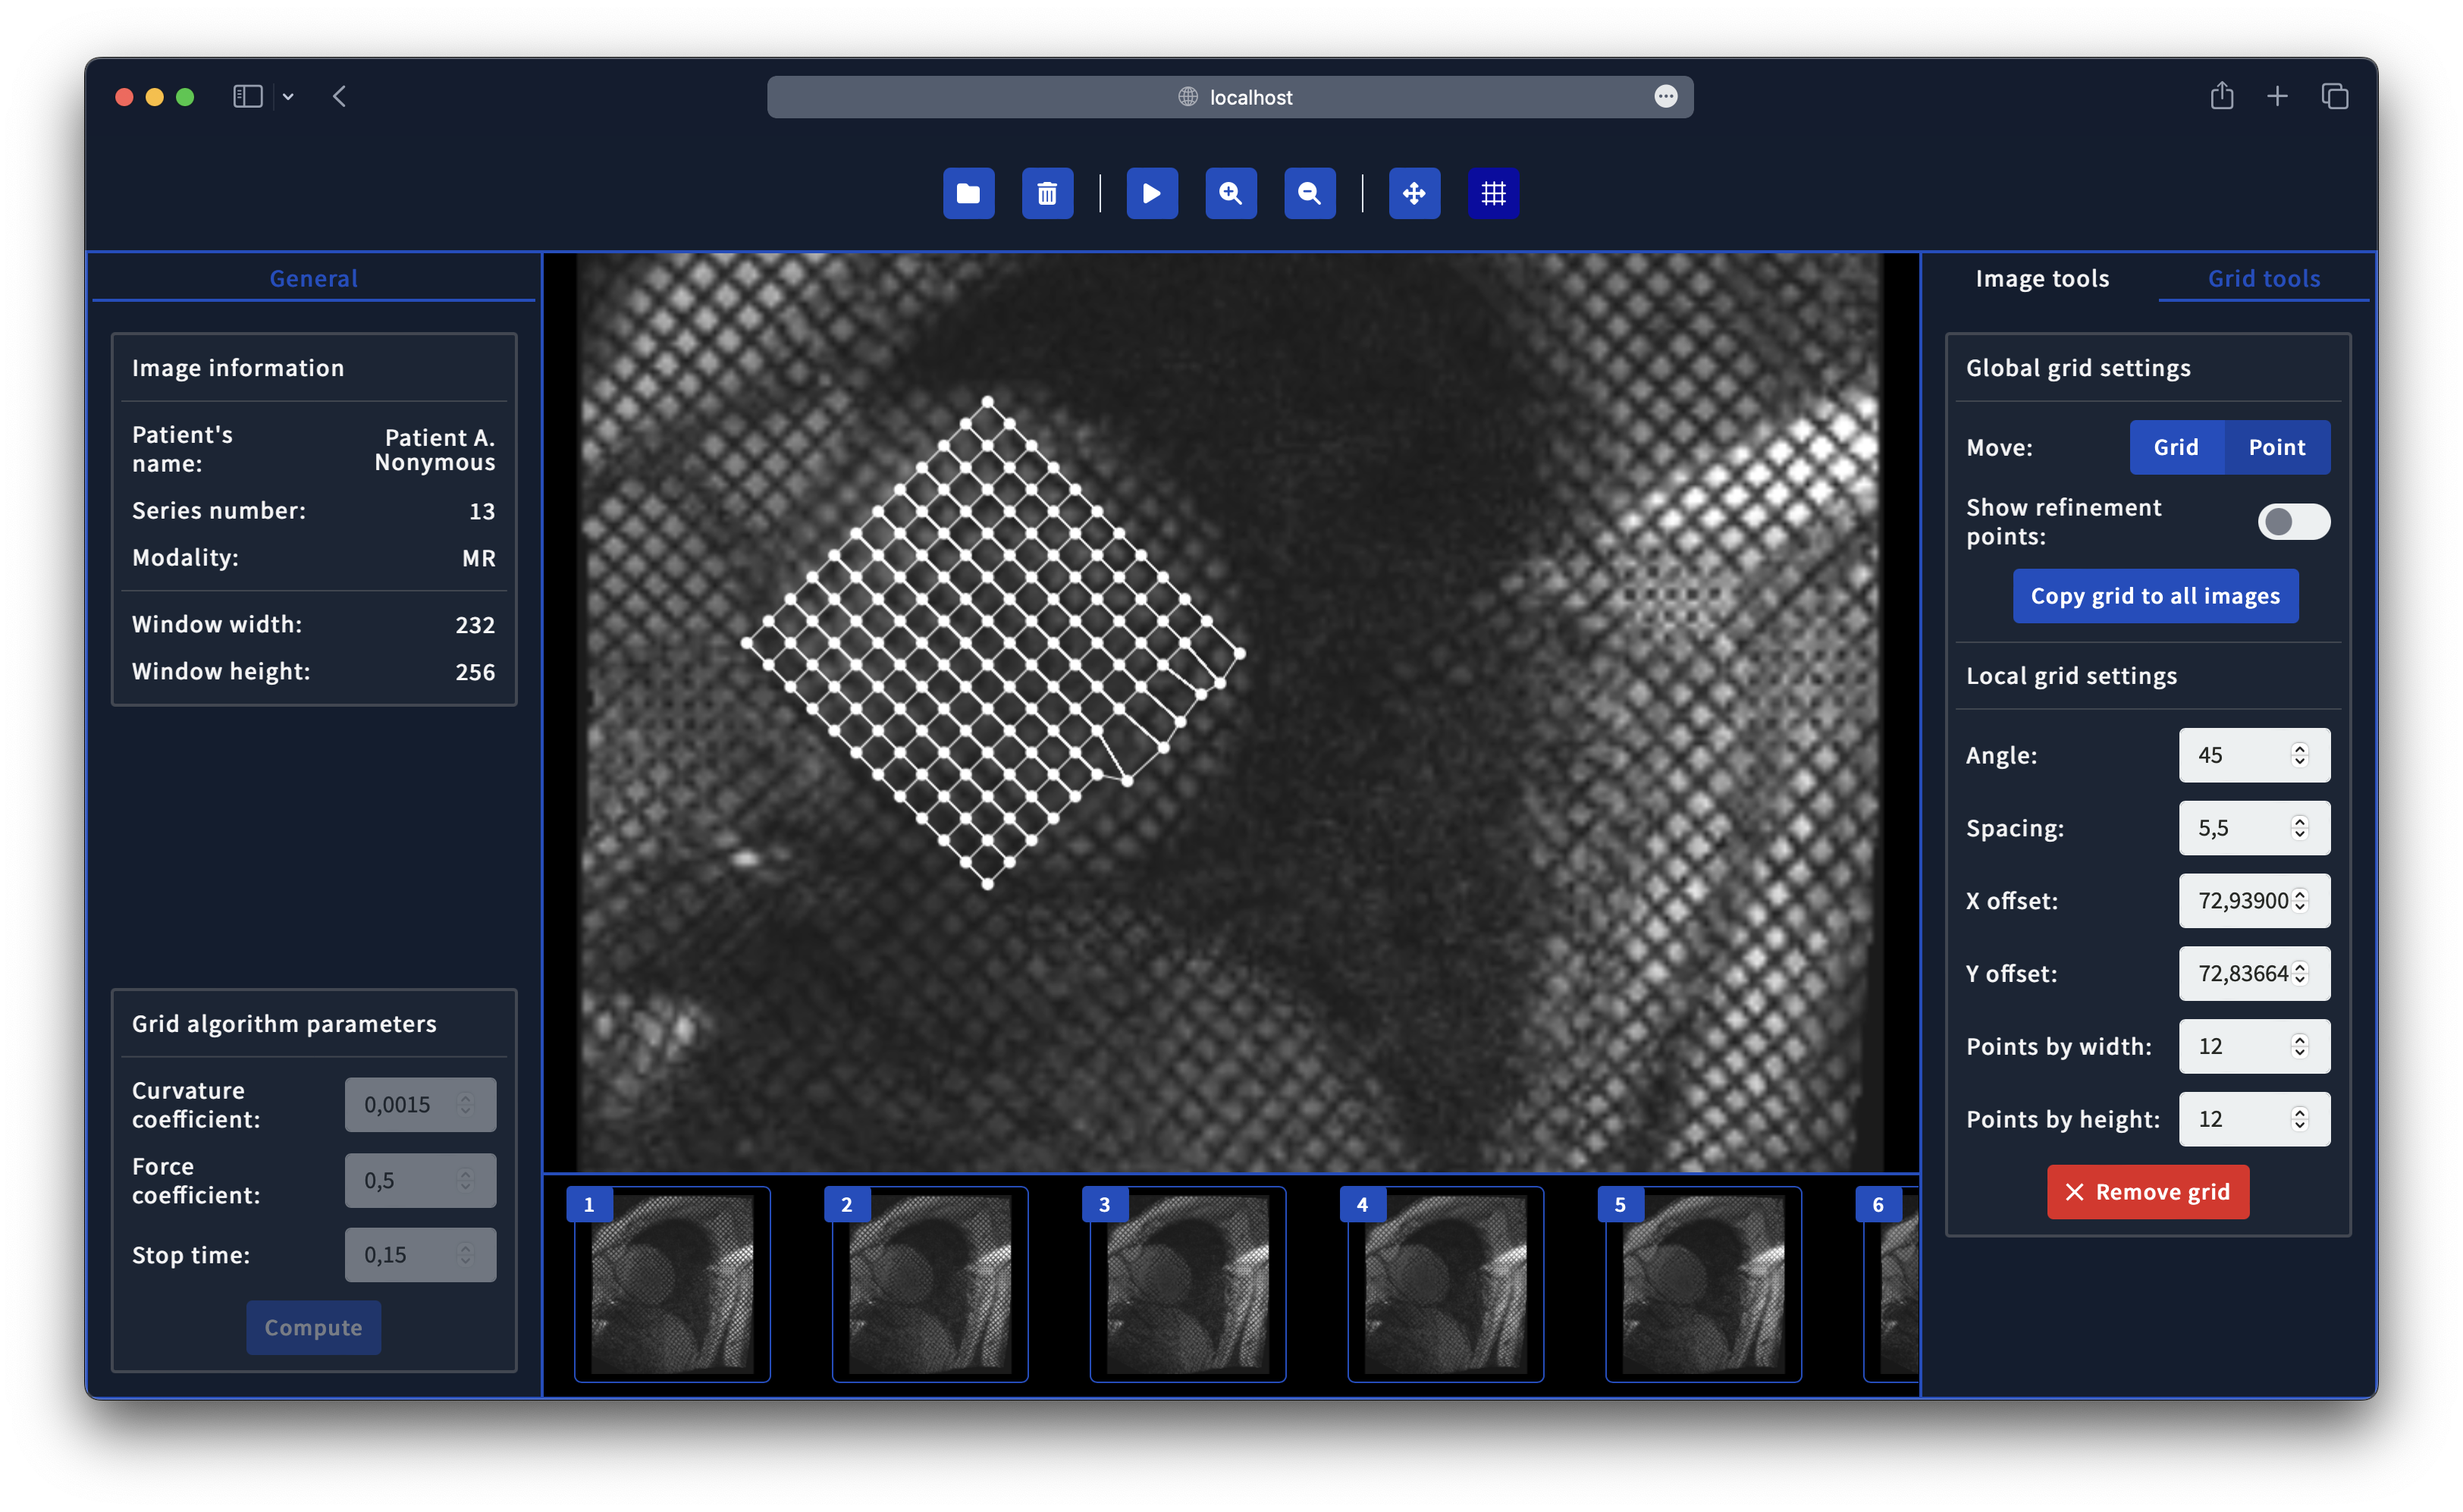
\includegraphics[height=9cm]{media/new_app/changed_points_coordinates.png}
        \captionsetup{justification=centering}
        \captionof{figure}{Snímka zobrazujúca zmenené koordináty niektorých bodov vykreslenej mriežky.}
\end {figure}

\begin {figure}[H]
        \centering
        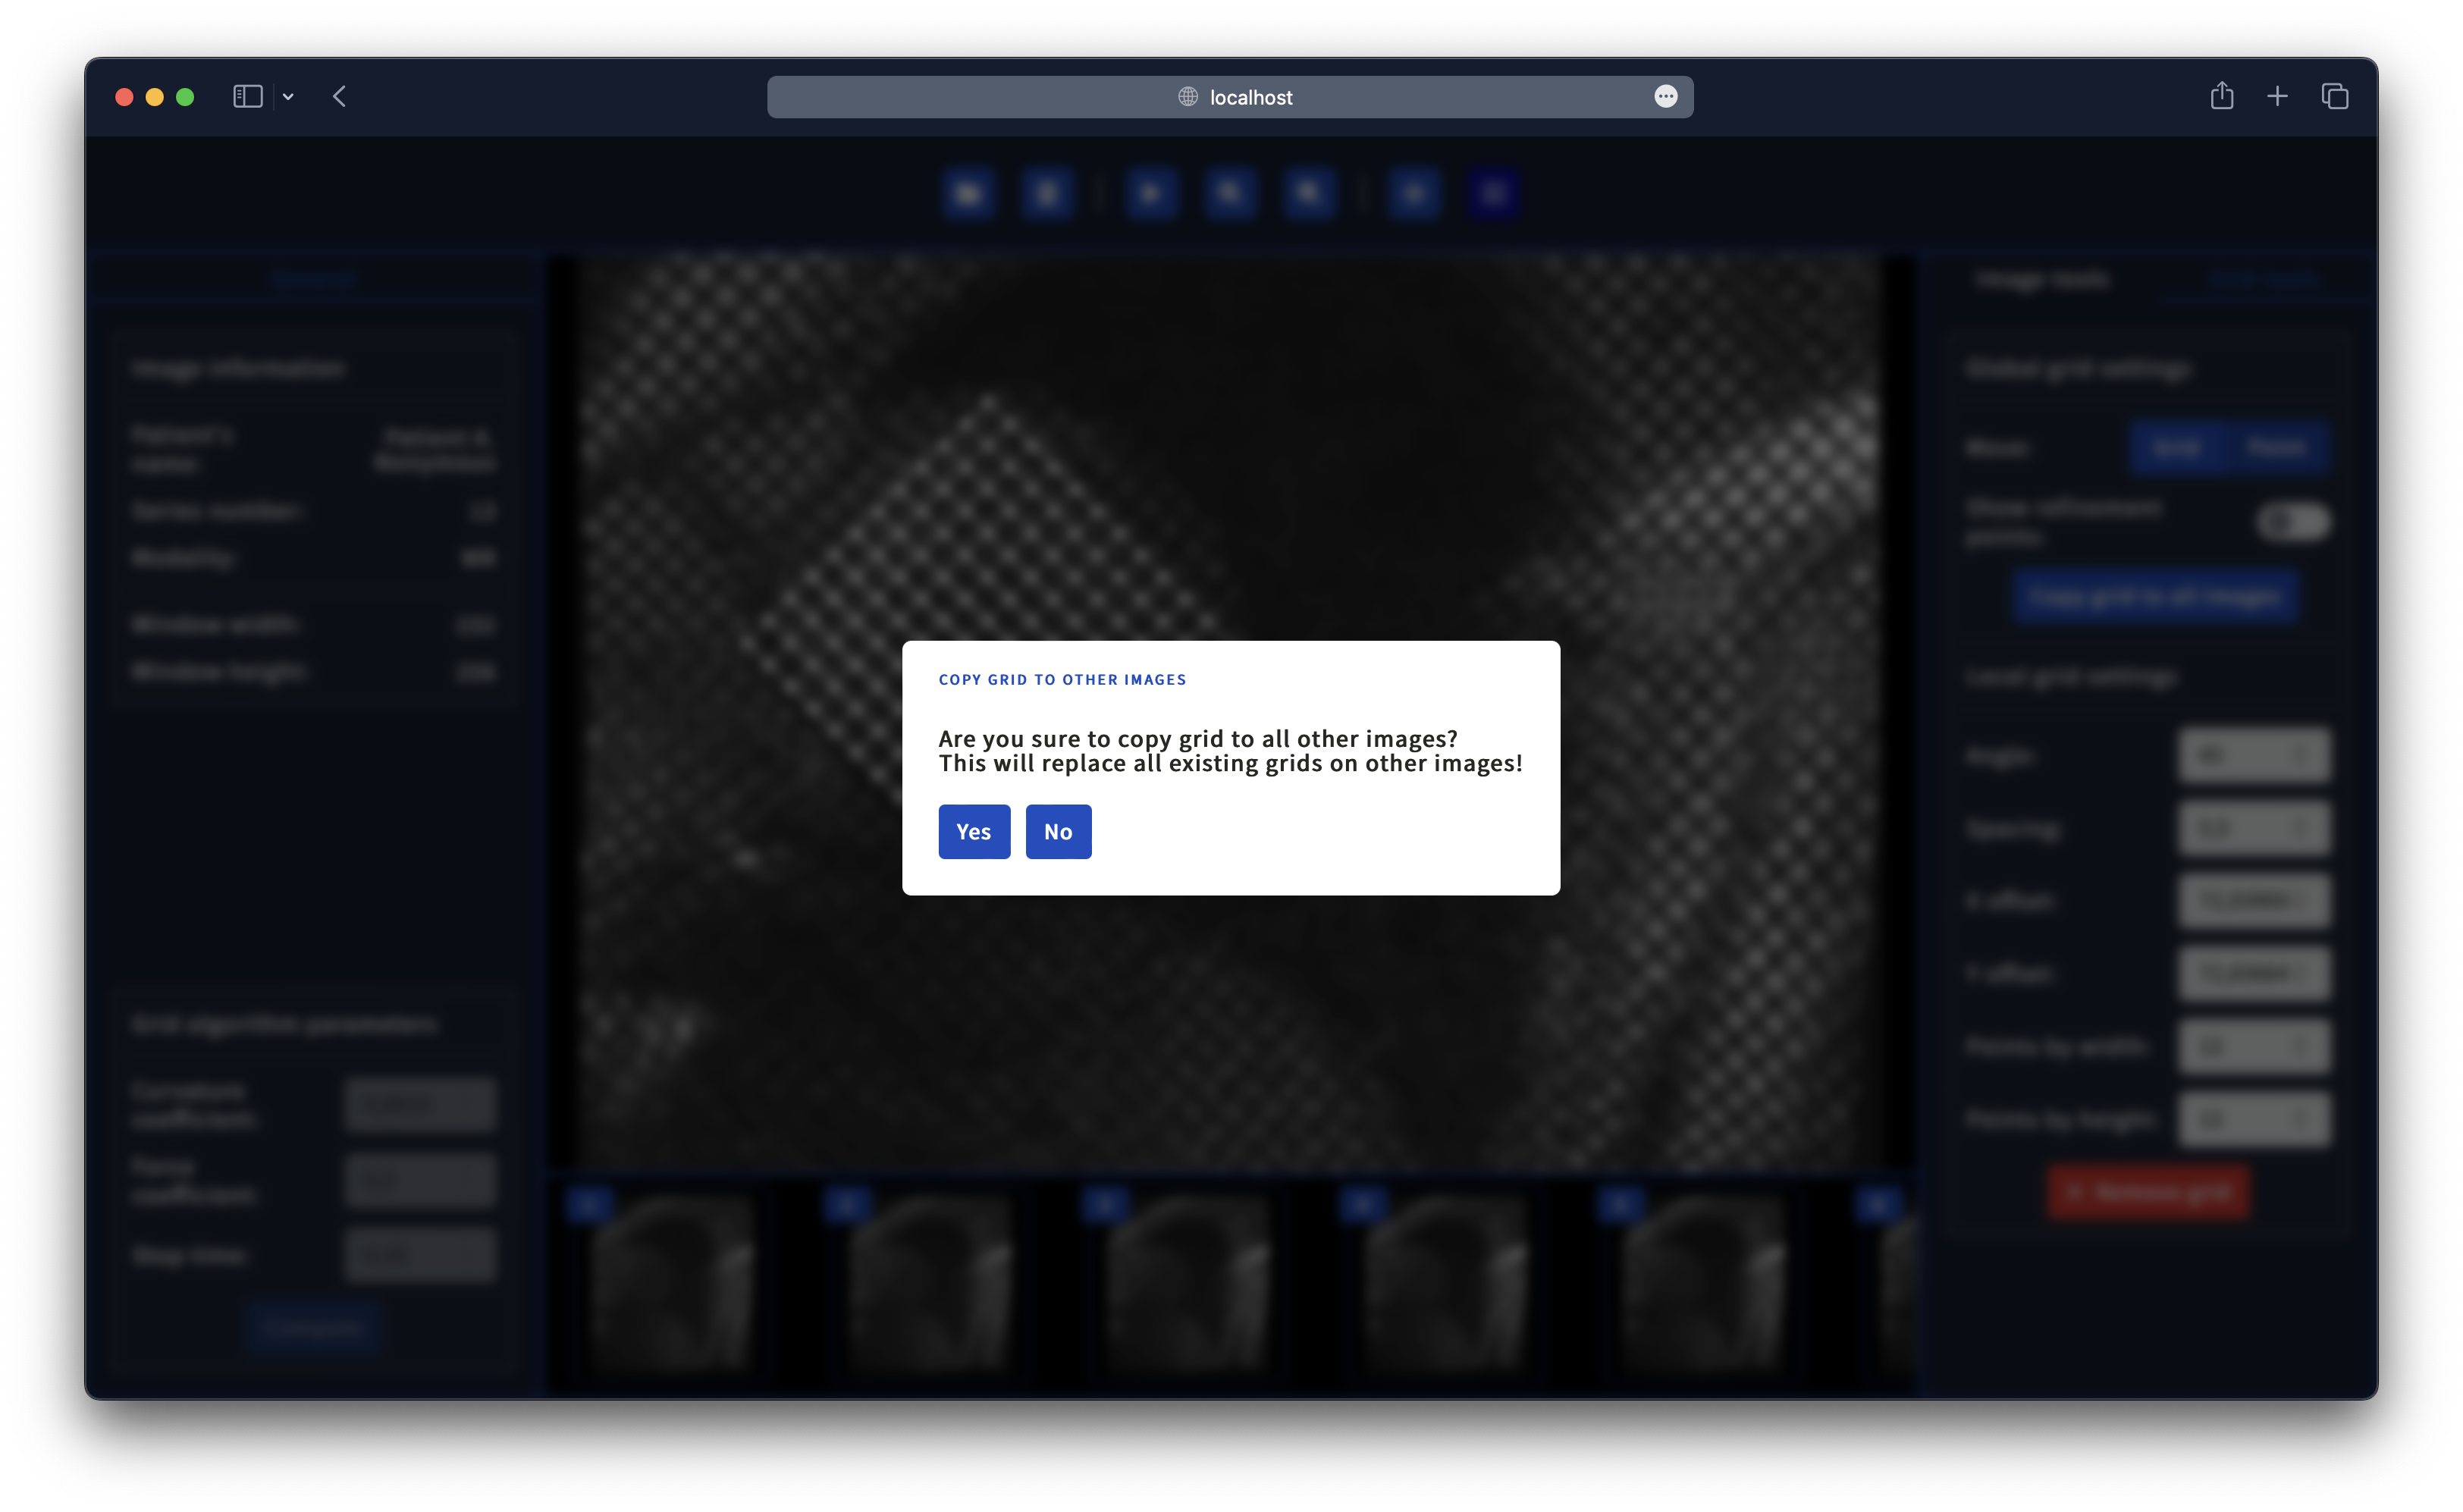
\includegraphics[height=9cm]{media/new_app/copy_grid_modal.png}
        \captionsetup{justification=centering}
        \captionof{figure}{Snímka zobrazujúca modálne okno, ktoré varuje pred prepísaním existujúcich mriežok vykreslených na ostatných DICOM snímkach, v prípade zvolenia možnosti skopírovania aktuálne zobrazenej mriežky do ostatných snímiek.}
\end {figure}
        \chapter{Obsah priloženého .zip súboru}

\begin{figure}
	\dirtree {%
		.1 diploma-thesis\DTcomment{adresár so zdrojovými kódmi}.
		.2 app\DTcomment{adresár so zdrojovými kódmi aplikácie}.
		.2 thesis\DTcomment{adresár so zdrojovým kódom práce vo formáte \LaTeX{}}.
		.3 DP\_Tomáš\_Taro\_2023.pdf\DTcomment{text práce vo formáte PDF}.
	}
\end{figure}

\end{document}
\end{document}
